\documentclass[12pt,a4paper]{article}
\usepackage[a4paper, 
            left=1.5in, 
            right=1.5in, 
            top=1in, 
            bottom=1in]{geometry} 
\usepackage{hyperref}
\usepackage[utf8]{inputenc}
\DeclareUnicodeCharacter{20B9}{\textrupee}
\usepackage{pgfplotstable}
\pgfplotsset{compat=1.18}
\usepackage{graphicx}
\usepackage{pifont}
\usepackage{longtable}
\usepackage{float}
\usepackage{geometry}
\usepackage{setspace}
\usepackage{amsmath}
\usepackage{array}
\usepackage{titlesec}
\usepackage{subcaption}
\usepackage{rotating}
\usepackage[style=ieee, sorting=none, citestyle=numeric-comp, backend=biber]{biblatex} % IEEE bibliography with numbered citations
\addbibresource{references.bib} % Your BibTeX file
\usepackage{forest}
\usepackage{tikz}
\usetikzlibrary{mindmap}
\usetikzlibrary{shadows}
\usepackage{glossaries}
\makeglossaries
\usepackage{makeidx}
\makeindex

\hypersetup{
    colorlinks=true,
    linkcolor=blue,
    filecolor=magenta,
    urlcolor=cyan,
    pdftitle={Project Report},
    pdfpagemode=FullScreen,
}


% Title

\title{
\vspace{7cm}
\textbf{Design and implementation of a multi-waveform function generator}

\\ P1 Requirements + Specifications
\\ + Design Cycle 1 + Design Cycle 2
\\ Monday Tribe
\\ Version : 4.2.1

}


\date{\today}

% Custom commands for abbreviations and glossary
\newcommand{\abbr}[2]{\textbf{#1} -- #2}
\newcommand{\term}[2]{\textbf{#1}: #2}

\begin{document}
\maketitle
\clearpage
% Table of Contents, List of Tables, and List of Figures
\pagenumbering{roman} % Use Roman numerals for the title page and ToC
\tableofcontents
\clearpage
\listoftables
\addcontentsline{toc}{section}{List of Tables}
\clearpage
\listoffigures
\addcontentsline{toc}{section}{List of Figures}

\clearpage
\section*{Index of Abbreviations}
\addcontentsline{toc}{section}{Index of Abbreviations}

\begin{longtable}{@{}p{0.3\textwidth}p{0.7\textwidth}@{}}
\textbf{\large Abbreviation} & \textbf{\large Expansion} \\\hline
\\[-0.5em] 
\textbf{SNR} \index{SNR} & \textbf{Signal to Noise Ratio} \index{Signal to Noise Ratio} \\
\\[-0.5em] 
\textbf{EMI} \index{EMI} & \textbf{Electromagnetic Interference} \index{Electromagnetic Interference} \\
\\[-0.5em]  
\textbf{LED} \index{LED} & \textbf{Light Emitting Diode} \index{Light Emitting Diode} \\
\\[-0.5em]  
\textbf{OLED} \index{OLED} & \textbf{Organic Light Emitting Diode} \index{Organic Light Emitting Diode} \\
\\[-0.5em]  
\textbf{I2C} \index{I2C} & \textbf{Inter-Integrated Circuit} \index{Inter-Integrated Circuit} \\
\\[-0.5em]  
\textbf{CAD} \index{CAD} & \textbf{Computer-Aided Design} \index{Computer-Aided Design} \\
\\[-0.5em]  
\textbf{IP} \index{IP} & \textbf{Ingress Protection} \index{Ingress Protection} \\
\\[-0.5em]  
\textbf{RH} \index{RH} & \textbf{Relative Humidity} \index{Relative Humidity} \\
\\[-0.5em]  
\textbf{TRL} \index{TRL} & \textbf{Technology Readiness Level} \index{Technology Readiness Level} \\
\\[-0.5em]  
\textbf{DOF} \index{DOF} & \textbf{Degree of Freedom} \index{Degree of Freedom} \\
\\[-0.5em]  
\textbf{ESP} \index{ESP} & \textbf{Espressif Systems Protocol} \index{Espressif Systems Protocol} \\
\\[-0.5em] 
\textbf{UI} \index{UI} & \textbf{User Interface} \index{User Interface} \\
\\[-0.5em]  
\caption{Index of Abbreviations} \label{tab:Index of abbreviations}
\end{longtable}

% Print the index at the end of the document


\clearpage

\newglossaryentry{EMI}
{
    name=EMI,
    description={Disturbance caused by electromagnetic signals affecting other devices}
}

\newglossaryentry{ATMega328p-AU}
{
    name=ATMega328p-AU,
    description={A low-power 8-bit microcontroller by Microchip, widely used in embedded systems for its efficiency, reliability, and compatibility with Arduino platforms}
}


\newglossaryentry{AD9833}
{
    name=AD9833,
    description={A low-power programmable waveform generator IC capable of producing sine, triangle, and square waves with high precision}
}
\newglossaryentry{BOM}
{
    name=BOM,
    description={A refined BOM in electrical engineering is an updated and detailed list of all materials, components, and parts required for a project, including specifications and quantities to ensure efficient assembly and procurement.}
}
\newglossaryentry{SPI}
{
    name=SPI,
    description={A high-speed communication protocol used for data exchange between microcontrollers and peripheral devices over short distances}
}
\newglossaryentry{HD44780}
{
    name=HD44780,
    description={A widely used LCD controller for 16x2 and 20x4 character displays, known for its ease of interfacing with microcontrollers}
}
\newglossaryentry{LM358}
{
    name=LM358,
    description={A general-purpose operational amplifier (op-amp) used for amplification, buffering, and signal conditioning in analog circuits}
}
\newglossaryentry{CAD}
{
    name=CAD,
    description={Software used to create precise 2D or 3D designs, technical drawings, and simulations for engineering and manufacturing}
}
\newglossaryentry{KiCad}
{
    name=KiCad,
    description={An open-source electronic design automation (EDA) tool used for creating schematics, PCB layouts, and circuit simulations}
}
\newglossaryentry{NE555}
{
    name=NE555,
    description={The NE555 is a versatile timer IC used for generating accurate time delays, oscillations, and pulse signals in electronic circuits, commonly used in timing, waveform generation, and signal processing applications.}
}
\newglossaryentry{ESP32}
{
    name=ESP32,
    description={A powerful microcontroller with integrated Wi-Fi and Bluetooth, designed for IoT applications, automation, and wireless communication}
}
\newglossaryentry{I2C}
{
    name=I2C,
    description={is a synchronous, multi-master, multi-slave serial communication protocol that uses two bidirectional lines, SCL (clock) and SDA (data), for low-speed data exchange. It is widely used in embedded systems to connect microcontrollers with sensors, memory chips, and other peripherals.}
}
\printglossary
\clearpage
\vspace{-1.5em}
\section*{List of Members}

\begin{longtable}{|l|l|l|l|}
\caption{List of members with corresponding IF} \label{tab:List of members with corresponding IF} \\ 
    \hline
    \textbf{Name} & \textbf{Entry Number} & \textbf{IF} & \textbf{Justification} \\ \hline
    \endfirsthead
    \hline
    \textbf{Name} & \textbf{Entry Number} & \textbf{IF} & \textbf{Justification} \\ \hline
    \endhead
    \hline
    \endfoot
    Name & Entry Number & IF & Justification \\ \hline
        Aarnav  Singh & 2022EE11161 & 1 & ~ \\ \hline
        Aarth Bhardwaj & 2022ee31747 & 0.59 & NRV \\ \hline
        Abdullah Tanveer & 2022EE11712 & 1 & ~ \\ \hline
        Abhineet Singh & 2022MT11736 & 0.88 & ~ \\ \hline
        Aditi Gaur & 2022MT11298 & 1 & ~ \\ \hline
        Aditya Nagarkar & 2022EE31224 & 1 & ~ \\ \hline
        Aditya Raj & 2022EE31760 & 0.59 & NRV \\ \hline
        Aditya vijay & 2022EE11166 & 1 & ~ \\ \hline
        Akarsh Gupta & 2022MT61966 & 0.86 & ~ \\ \hline
        Aman Gupta & 2022EE11808 & 1 & ~ \\ \hline
        Anany Mishra & 2022MT61965 & 1 & ~ \\ \hline
        Anish kumar & 2022EE11708 & 0.74 & PCT \\ \hline
        Ankur Khetan & 2022EE31753 & 1 & ~ \\ \hline
        Apoorva Prashant Jain & 2022EE11657 & 1 & ~ \\ \hline
        Arpit Moga & 2022EE31777 & 1 & ~ \\ \hline
        Arunim & 2022EE32002 & 1 & ~ \\ \hline
        Aryan Jangra & 2022EE11716 & 1 & ~ \\ \hline
        Aryan Sharma & 2021EE10141 & 0 & NRV \\ \hline
        Aryan Verma & 2022EE11671 & 1 & ~ \\ \hline
        Astha Lohia & 2022MT11927 & 1 & ~ \\ \hline
        Ayush Jagatramka & 2021MT10286 & 1 & ~ \\ \hline
        C VARSHITH REDDY & 2022EE11693 & 1 & ~ \\ \hline
        Chandan Kumar Thakur & 2022EE31773 & 0.98 & ~ \\ \hline
        Deepak Kumar Jha & 2021MT10233 & 0.4 & NRV \\ \hline
        Dev Elvis Kannath & 2022MT61961 & 0.98 & ~ \\ \hline
        Dev Sharma & 2022EE31308 & 1 & ~ \\ \hline
        Dhanashri Shivdas & 2022EE31907 & 1 & ~ \\ \hline
        Dheeraj HJ & 2022EE11704 & 0.94 & ~ \\ \hline
        Dhruv Belawat & 2022EE11661 & 1 & ~ \\ \hline
        Divyansh Raj Sinha & 2022EE31194 & 0.98 & ~ \\ \hline
        Divyanshu Pal & 2022MT11295 & 0.55 & NRV \\ \hline
        Gandharva Chhipa & 2022EE11663 & 1 & ~ \\ \hline
        Hariom & 2022EE11697 & 1 & ~ \\ \hline
        Harshit Baraskar & 2022EE31769 & 1 & ~ \\ \hline
        Hitesh Yadav & 2022MT11322 & 1 & ~ \\ \hline
        Ishaan Lakhotiya & 2022EE11677 & 1 & ~ \\ \hline
        Ishu Rajput & 2022EE11173 & 1 & ~ \\ \hline
        Jaipal & 2022EE11705 & 0 & NRV \\ \hline
        Jay Kumar & 2022EE31781 & 0.71 & PCT \\ \hline
        Jaya Chauhan & 2022EE31786 & 1 & ~ \\ \hline
        Jitendra Meena & 2022EE31787 & 0 & NRV \\ \hline
        Kalangi Sai Venkata Krishna Sendhvil & 2022EE11700 & 1 & ~ \\ \hline
        Kartikey Agarwal & 2022EE11156 & 1 & ~ \\ \hline
        Krishna Gopal Agarwal & 2022EE31762 & 0.51 & NRV \\ \hline
        Kriti Garg & 2022EE11684 & 1 & ~ \\ \hline
        Lisha Goel & 2022EE11685 & 1 & ~ \\ \hline
        Madhav Gupta & 2022EE11737 & 1 & ~ \\ \hline
        Manas Singla & 2021MT10599 & 1 & ~ \\ \hline
        Mayank Agarwal & 2022EE31759 & 0.76 & PCT \\ \hline
        Mayank kumar jha & 2022EE11673 & 1 & ~ \\ \hline
        Mitali Bhagat & 2020MT10821 & 1 & ~ \\ \hline
        Naman Goel & 2022MT11272 & 1 & ~ \\ \hline
        Naveen Kumar Raypuriya & 2022EE11181 & 0 & NRV \\ \hline
        Prabhjit Singh & 2022EE11720 & 0.98 & ~ \\ \hline
        Pratyush Agrawal & 2022EE11158 & 1 & ~ \\ \hline
        Rakshit Sohlot & 2022MT11919 & 1 & ~ \\ \hline
        Rinku Meena & 2022EE11187 & 0 & NRV \\ \hline
        Rishit Jaiswal & 2022EE31771 & 0.71 & PCT \\ \hline
        Rohan Chaturvedi & 2022MT11262 & 1 & ~ \\ \hline
        Rohan Roy & 2022MT11294 & 0.94 & ~ \\ \hline
        Rohit Shaw & 2022MT61988 & 0 & NRV \\ \hline
        Saem Habeeb & 2022MT62004 & 1 & ~ \\ \hline
        Sahaj Jain & 2022EE31741 & 0.79 & PCT \\ \hline
        Samyak Jain & 2022MT11658 & 0.92 & ~ \\ \hline
        Sanchit Jindal & 2022EE31738 & 1 & ~ \\ \hline
        Shubham Singh & 2022EE11725 & 1 & ~ \\ \hline
        Sunrit Roy Karmakar & 2021MT10702 & 1 & ~ \\ \hline
        Sushant kumar & 2022EE12045 & 1 & ~ \\ \hline
        Teekam singh & 2022EE31770 & 0.88 & ~ \\ \hline
        Tejas & 2022EE31199 & 0.83 & ~ \\ \hline
        Tushar Verma & 2022EE31742 & 1 & ~ \\ \hline
        Ujjawal meena & 2022EE11733 & 1 & ~ \\ \hline
        Vaibhav Ahuja & 2022EE11839 & 1 & ~ \\ \hline
        Vamika & 2022EE11182 & 0.94 & ~ \\ \hline
        Vatsal Jain & 2022EE11672 & 1 & ~ \\ \hline
        Vikas Kumar & 2022EE11149 & 0.94 & ~ \\ \hline
        Vinit Shende & 2021MT10260 & 1 & ~ \\ \hline
        Vipul & 2022EE31198 & 0.94 & ~ \\ \hline
        Yadvendra Gurjar & 2022EE31764 & 0.74 & PCT \\ \hline
        Yagya Goyal & 2022EE11157 & 1 & ~ \\ \hline
\end{longtable}

\textbf{NRV : }No responses to emails or messages were received. Did not come forward to volunteer.

\textbf{PCT : }Partial completion of allotted tasks.

% Start main content
\pagenumbering{arabic} % Switch to Arabic numerals for the main content
\clearpage
\begin{abstract}

This project aims to design and develop a cost-effective, user-friendly function generator.
\newline
\textbf{Core Functions}
\begin{itemize}
  \item Multiple waveform generation (Square, Ramp, Triangular, Sine with DC offset) \parencite{bkprecision_function_generator_guide}
  \item Adjustable duty cycle for PWM demonstration \parencite{bhavanishankar2021design}
  \item frequency range from 0.1 Hz to 1 MHz and an amplitude range of 10 V peak to peak \parencite{functionGenerator}
  \item Using input power supply 5V DC, then using a boost converter module (MT3608) to step it up to 15V
  \item Creating a voltage inverter using NE555 Timer to get a -5V and -15V voltage for the reest of the circuitry
  \item External oscillator compatibility
  \item Constant output impedance regardless of circuit impedance \parencite{rgpv_signal_generator}
\end{itemize}
\textbf{Safety Features}
\begin{itemize}
  \item Short-circuit and overcurrent protection
  \item Grounded metal body
  \item ESD protection
  \item Isolated channel design
\end{itemize}
\textbf{Design Specifications}
\begin{itemize}
  \item Industry-standard dimensions \parencite{iec60297_3_100_2008} (W212 x H114 x D283 mm)\parencite{scientech4064s}
  \item Operating conditions: 0-40°C, 85\% Relative Humidity \parencite{scientech4064s}
  \item OLED display with wide viewing angle
  \item Front panel controls with coarse/fine-tuning
  \item IP20 \parencite{isolite_ip_rating_chart} protection rating with robust insulation, and thermal stability under varying laboratory conditions
\end{itemize}
The design prioritizes student learning by providing essential functionality without overwhelming complexity. Built-in safety features and robust construction ensure reliability in a laboratory environment. The project addresses the need for cost-effective, educational-focused test equipment.
\end{abstract}
\clearpage

\section{Motivation}
\setstretch{1.5}
% Motivation content here.
\begin{quote}
    % \textit{`` Simplicity is the ultimate sophistication.''}  
    % \hfill -- Leonardo da Vinci

    \textit{``Simplicity is the ultimate sophistication.''}  
    \hfill -- Leonardo da Vinci\\
\end{quote}

The \textbf{primary objective} of this project is to design and develop a function generator tailored to the specific needs of students enrolled in the ELP101 Basic Electronics Laboratory \parencite{dixit_lab_manual}. Recognizing that these students are at the beginning of their journey in electronics, we aim to create an intuitive, \textit{cost-effective} device focused on fundamental functionality.\\
Commercial function generators have features which are not needed for ELP101 level experiments. Our function generator will address this by offering essential waveform generation capabilities—such as sine, square, and triangular waves—while maintaining simplicity and reliability suitable for a ELP101 laboratory environment.\\
Beyond supporting standard laboratory experiments, the device's affordability will attract the beginner and encourage experimentation.

\begin{quote}
    \textit{Our ultimate goal is to enhance the ELP101 lab experience, making it more engaging and effective, while cultivating a passion for electronics among first-year students.}
\end{quote}

\section{Requirements}
\subsection{Technical Requirements}
\parencite{functionGenerator}
\parencite{scientech4064s}
\parencite{scientific_mes_technik_2015}
\parencite{rgpv_signal_generator}
\begin{itemize}

  \item Functions: Square (Duty cycle), Ramp, Triangular, Sine (with a DC offset)

  \item Frequency range: 0.1Hz - 1MHz
  \item Amplitude range: 10V peak-to-peak
  \item Error Bound:
  \parencite{tektronix_cfg253_1993}
  \begin{itemize}
    \item Till 100 Hz: ±0.1 Hz
    \item 100--1 kHz: ±1 Hz
    \item 1 kHz--10 kHz: ±10 Hz
    \item 10 kHz--100 kHz: ±100 Hz
    \item 100 kHz--1 MHz: ±1 kHz
  \end{itemize}

  \item No. of output channels: 1
  
  \item Constant Output produced irrespective of external circuit impedance
(reliable signal for experiments, ensuring consistency even when the connected circuit has varying impedance) \parencite{bhavanishankar2021design}
  \item Output Port(Sync Port), within metallic box connected to the ground to prevent EMI interference 
  \item SNR ratio/ Noise rejection
  \item DC offset range: 12V - 15V


\end{itemize}

\subsubsection{Safety features}
\begin{itemize}
    \item Short-circuit protection / Overcurrent protection
    \item Metal body grounded
    \item Electrostatic discharge protection
\end{itemize}

\subsubsection{Design}
\begin{itemize}
    \item OLED
    \item $90^\circ$ angle power cable
    \item Coarse tuning and fine tuning
\end{itemize}

\subsubsection{Display}
\begin{itemize}
    \item Function display
    \item Frequency display
    \item Amplitude value display
    \item Monochrome
    \item Wide angle view, OLED Screen

\end{itemize}

\subsubsection{Power}
\begin{itemize}
    \item Stable conversion with output voltage ripple:
    \begin{itemize}
        \item \textbf{Light Load (50mA):} 30--50mV
        \item \textbf{Medium Load (200mA):} 50--100mV
        \item \textbf{Heavy Load (1A):} 100--200mV
        \item \textbf{Insufficient Output Capacitance:} \textgreater 200mV (unstable)
    \end{itemize}
    \item Wire at 90 degrees (structural component)
\end{itemize}

\subsubsection{Front Panel}
\begin{itemize}
    \item Finite rotation knob (0 to 270 degrees)
    \item Arrow on the knob (provides clear direction for adjustments)
    \item Use of Joystick (Simplifies setting a wide frequency range without excessive knob rotation)
    \item Easy-to-understand buttons (buttons should specify their functions)
    \item Power ON button should be on the front panel (not on top/sides, as there will then be a problem in stacking on the rack of standard dimensions)
\end{itemize}


\subsection{Structural Requirements}
\begin{itemize}
    \item Insulated
    \item Gaskets and aluminum foil are used to shield the device from \gls{EMI} Interference
    \item The circuit should fit inside the box with heat sinks and padding
    \item Dimensions: W 212 X H 114 X D 283 (9 inch / 19 inch industry standard) \parencite{iec60297_3_100_2008}
    \item Holes should be present so that no additional cooling equipment is required
    \item Both horizontal and vertical degrees of freedom allow for flexible positioning on lab benches or racks and allow for direct viewing even when the function generator is positioned sideways
    \item The casing is made of acrylic, which is heated to 85° Celsius. As a result, when near amplifiers and other heat sources, ensure adequate ventilation by including air vents or heat sinks in the design and using thermal insulating spacers between the acrylic walls and heat-generating components. 
    \item A change in temperature shouldn't affect the mechanical qualities
    \item Operating Conditions: 0-40 °C, 85\% RH \parencite{scientech4064s}
    \item Making use of speaker connections to ensure a steady and dependable input supply connection
    \item The first digit for solids and the second digit for water should match IP 20. \parencite{isolite_ip_rating_chart}
    \item  Comprising 500g of the case, 750g of the circuitry, 250g of the transformer adapter, 250g of the switches and knobs, and other miscellaneous  \parencite{scientech4064s}
\end{itemize}











\section{Specifications}
\subsection{Front Panel Layouts and Controls}
\subsubsection{Frequency Controls}
\begin{itemize}
    \item \textbf{Primary Control:} Joystick with Push Button \begin{itemize}
        \item Press the joystick to select a digit.
        \item The OLED display shows the selected frequency.
    \end{itemize}
    \item \textbf{Frequency Range Selector:}
    \begin{itemize}
        \item Adjust frequency using the joystick
        \item A blinking cursor indicates when a particular digit is being modified.
    \end{itemize}
\end{itemize}


\subsubsection{Amplitude Control}
\begin{itemize}
    \item \textbf{Dedicated Potentiometer:}
    \begin{itemize}
        \item Adjustable range: 0V to 9V peak-to-peak.
    \end{itemize}
    \item \textbf{Fine/Coarse Adjustment Switch:}
    \begin{itemize}
        \item \textbf{Fine:} Enables precise amplitude adjustments.
        \item \textbf{Coarse:} Allows rapid amplitude changes.
    \end{itemize}
\end{itemize}

\subsubsection{DC Offset Control}
\begin{itemize}
    \item \textbf{Offset Potentiometer:}
    \begin{itemize}
        \item Adjustable range: ±12V
        \item Center detent at 0V for easy adjustment
        \item Calibrated scale markings for precise tuning
    \end{itemize}
    \item \textbf{Offset ON/OFF Switch:}
    \begin{itemize}
        \item Toggles DC offset activation.
        \item LED indicator illuminates when offset is active.
    \end{itemize}
\end{itemize}

\subsubsection{Display and Indicators}
\begin{itemize}
    \item \textbf{0.96 inch OLED Display:} The display provides the following information: \begin{itemize}
        \item Current frequency
        \item Waveform type
        \item Output status
        \item Amplitude setting
    \end{itemize}
\end{itemize}

\subsubsection{Output Controls}
\begin{itemize}
    \item \textbf{Output Power Switch} 
    \item \textbf{Ground Terminal}
    \item \textbf{Selectable Waveforms (via menu):}
    \begin{itemize}
        \item Sine
        \item Triangle
        \item Square
    \end{itemize}
\end{itemize}

\subsubsection{Front Panel Layout Specifications}
\begin{itemize}
    \item \textbf{Dimensions:} 
    \begin{itemize}
        \item Width $\times$ Height $\times$ Depth: \textbf{19 cm $\times$ 8 cm $\times$ 26 cm}
        \item Knob Diameter (for DC Offset and Amplitude Variation): \textbf{0.8 cm}
        \item Joystick Diameter (for Frequency Control): \textbf{1 cm} 
        \item Extruded Front Panel Thickness: \textbf{0.5 cm}
        \item Power Supply Dimensions: \textbf{2.8 cm $\times$ 3.1 cm}
        \item Push Button Dimensions (Diameter $\times$ Thickness): \textbf{1 cm $\times$ 0.1 cm}
    \end{itemize}
\end{itemize}


\subsection{Core Components}
\subsubsection{ESP32 Microcontroller}
    \begin{itemize}
        \item \textbf{Input:} Push Buttons, Joystick signals
        \item \textbf{Output:} OLED control signals, \gls{SPI} communication to AD9833
        \item \textbf{Function:} Controls overall system operation, processes user inputs, configures waveform generator
    \end{itemize}
    
\subsubsection{\gls{AD9833} Function Generator IC}
\begin{itemize}
    \item \textbf{Input:} Supply voltage: 2.3 V to 5.5 V, DC power, 25 MHz clock signal
    \item \textbf{Output:} Frequency range up to 1 MHz,  
          \begin{itemize}
              \item Sine wave: 0.65 V peak-to-peak
              \item Triangle wave: 0.65 V peak-to-peak
          \end{itemize}
    \item \textbf{Function:} Programmable frequency and phase control, generates basic waveforms
\end{itemize}
    
\subsubsection{0.96 Inch \gls{I2C}/IIC 4pin OLED Display Module}
    \begin{itemize}
        \item \textbf{Input:} 3.3V DC power, I2C data from microcontroller
        \item \textbf{Output:} Displays selected waveform type and output status (ON/OFF)
        \item \textbf{Function:} Real-time parameter display
    \end{itemize}
    
\subsubsection{Joystick with Integrated Switch}
    \begin{itemize}
        \item \textbf{Input:} User movement and button press
        \item \textbf{Output:} Analog signals to the microcontroller
        \item \textbf{Function:} Adjusts frequency values, toggles output waveform
    \end{itemize}
    
\subsubsection{\gls{LM358} Operational Amplifier}
\begin{itemize}
    \item \textbf{Input:} Power supply
    \item \textbf{Output:} DC offset/amplification
\end{itemize}
    
\subsection{Power Specifications}

\begin{enumerate}
    \item \textbf{Power Input}
    \begin{itemize}
        \item \textbf{Voltage Requirement:}
        \begin{itemize}
            \item \textbf{DC Input} 5 V DC from an external adapter(connected via 4 pin speaker connector), in parallel to a C-port input power
        \end{itemize}
        \item \textbf{Power Consumption:} Designed to operate within a power range of 10-50 W. 
    \end{itemize}

    \item \textbf{Output Signal Specifications}
    \begin{itemize}
        \item \textbf{Amplitude Range (Peak-to-Peak Voltage):}Max 10 V peak-to-peak 
        \item \textbf{Maximum Output Power:} Typically ranges between 0.5 W and 2 W for low-frequency generators .
        \item \textbf{Load Impedance:} Standard 50  $\Omega$.
    \end{itemize}

    \item \textbf{Environmental Power Considerations}
    \begin{itemize}
        \item \textbf{Operating Temperature:} Usually 0 °C to 40 °C
        \item \textbf{Storage Temperature:} Typically -20 °C to 60 °C
    \end{itemize}
\end{enumerate}

\subsection{Cost Specifications}

    \begin{table}[h]
    \centering
    \begin{tabular}{|l|c|l|}
        \hline
        \textbf{Component} & \textbf{Cost (INR)} & \textbf{Link} \\
        \hline
      AD9833 & 249 & \href{https://robu.in/product/programmable-microprocessors-serial-interface-module-ad9833/?gad_source=1&gbraid=0AAAAADvLFWflraTKBAXcXi8lcRZeiv1KN								
}{Buy Here} \\
        Push Buttons x5Pcs Needed & 25 & \href{https://robu.in/product/6x6x8mm-tactile-push-button-switch-pack-of-20/?gad_source=1&gclid=Cj0KCQiA19e8BhCVARIsALpFMgHyHX2kIliyaSVVKPDi2JRiuor1n_hnvSvxT6yi8Bzhh5RgaAjEDrAaAjyLEALw_wcB										
}{Buy Here} \\
        PS2 Joystick Module Breakout Sensor & 30 & \href{https://robu.in/product/joystick-module-ps2-breakout-sensor/			
}{Buy Here} \\
        10k Potentiometer & 28.32 & \href{https://quartzcomponents.com/products/10k-potentiometer?variant=37780629029048&country=IN&currency=INR&utm_medium=product_sync&utm_source=google&utm_content=sag_organic&utm_campaign=sag_organic?utm_source=google&utm_medium=FreeListings&gad_source=1&gbraid=0AAAAACPPFdOYQYKuLK6Di4bmruTBRNibj										
}{Buy Here} \\
        \gls{NE555} timer & 16 & \href{https://www.flyrobo.in/ne555-timer-ic-555-timer-ic-other?tracking=ads&tracking=4a9a9a&gad_source=1&gclid=Cj0KCQiA19e8BhCVARIsALpFMgEkYDUMl-UfirUTmGpzuVR5kTlrXqLOQ60ygaDCPA6CEetvGh51pAUaAr-PEALw_wcB										
}{Buy Here} \\
        BNC Male Connector Plug & 25 & \href{https://www.indiamart.com/proddetail/bnc-male-connector-plug-crimp-type-for-coaxial-cable-22246828848.html						
}{Buy Here} \\
        Boost converter MT3608 & 32 & \href{https://www.ktron.in/product/mt3608-step-up-module-without-usb/?utm_term&utm_campaign=smartShoppingAds4&utm_source=adwords&utm_medium=ppc&hsa_acc=6332829093&hsa_cam=18276269511&hsa_grp&hsa_ad&hsa_src=x&hsa_tgt&hsa_kw&hsa_mt&hsa_net=adwords&hsa_ver=3&gad_source=1&gclid=Cj0KCQiA19e8BhCVARIsALpFMgGCfpkLpQZs-0B8qRVIAdGf1CMT3q_tUfk5yHe0RDb73FAUCvlW0HIaAsclEALw_wcB&v=c86ee0d9d7ed										}{Buy Here} \\
        Opamp (LM358) & 20 & \href{https://robu.in/product/lm358dr-texas-instruments-operational-amplifier-2-amplifier-700-khz-0-4-v-%C2%B5s-%C2%B1-1-5v-to-%C2%B1-16v-soic-8-pins/?gQT=1										}{Buy Here} \\
        Resistors (various) & 20 & \href{https://robu.in/product-category/electronic-components/resistors/carbon-resistors/				}{Buy Here} \\
        Capacitors (various) & 16 & \href{https://robu.in/product-category/electronic-components/capacitor/ceramic-capacitors/				}{Buy Here} \\
        1N4148 diode & 24 & \href{https://robu.in/product/1n4148-multicomp-pro-1n4148-diode-ultrafast-recovery-150ma-75v-do-204ah-2/?gad_source=1&gclid=Cj0KCQiA19e8BhCVARIsALpFMgHX-qOd0qXdqmdy3eUi2-WL5AJRoWwls-3BIyJW_2mFxNwJz4MY8nAaAmYiEALw_wcB										}{Buy Here} \\
        100uF cap & 12 & \href{https://robu.in/product/ers1em101e11ot-aishi-100uf-25v-%C2%B120-plugind6-3xl11mm-aluminum-electrolytic-capacitors-leaded-rohs/?gad_source=1&gclid=Cj0KCQiA19e8BhCVARIsALpFMgErKTPNtk2IiqtYgltPr4PTWOH6o-FX0y98wrfIQv1PBB3dJaxZpY8aAvlsEALw_wcB										}{Buy Here} \\
        47nF cap & 9 & \href{https://robu.in/product/47nf-0-047uf-2a473j-100v-polyester-film-capacitor-pack-of-10/?gad_source=1&gclid=Cj0KCQiA19e8BhCVARIsALpFMgHfLoV9aubSuMPaubS65butA6_7AWVT8UYiebUv4usozKw8f5bLz-waApPnEALw_wcB}{Buy Here} \\
        3.3Kohm & 9 & \href{https://robocraze.com/products/3-3k-ohm-resistor-pack-of-10?variant=40194239168665&country=IN&currency=INR&utm_medium=product_sync&utm_source=google&utm_content=sag_organic&utm_campaign=sag_organic&campaignid=21586511453&adgroupid=&keyword=&device=c&gad_source=1&gclid=Cj0KCQiA19e8BhCVARIsALpFMgG6zi3UZVodyrypSKhDbTbAKKFpjDyVXMNTIVhEQpIBouNSHAr6oTgaAkBwEALw_wcB										}{Buy Here} \\
        1Kohm & 1 & \href{https://robu.in/product/1k-ohm-0-25w-metal-film-resistor-pack-of-100/?gad_source=1&gclid=Cj0KCQiA19e8BhCVARIsALpFMgGkjHfa3u916-HJpiEMx3V5_nYZM5VjXJVQzkSA9NVTIj2CspmWaX8aAicTEALw_wcB										}{Buy Here} \\
        Female C to 4 pin & 1 & \href{https://electronicspices.com/product/usb-3-1-type-c-4-pin-female-connector-with-data-and-charging-port}{Buy Here} \\
        ESP32 & 260 & \href{https://ebhoot.in/shop-2/esp-wifi-boards/esp32-node-mcu-development-board-with-wifi-and-bluetooth-cp2102-driver-30-pin/}{Buy Here} \\
        OLED & 139 & \href{https://robu.in/product/4pin-oled-display-module-blue-color/?gad_source=1}{Buy Here} \\
        Acrylic sheets (2mm×1ft×1ft) & 160 & \href{https://www.indiamart.com/proddetail/2-mm-colored-acrylic-sheet-11916138862.html?prdnmfrm=1}{Buy Here} \\
        \hline
        Total Cost & 1076.32 & \\
      \hline
    \end{tabular}
    \caption{Component Cost Table}
    \label{tab:component-cost}
\end{table}

\subsection{Technology Readiness Level}
% \subsubsecion{TRL 7}
    \begin{itemize}
        \item \textbf{TRL 7:} Prototype demonstration in real operational conditions
        \item Tests the technology under radiations and extreme temperature levels, demonstrating its functionality and reliability
        \item This stage confirms readiness for full-scale mission integration
    \end{itemize}

\clearpage
% References (if applicable)

\subsection{Man Hour Specifications}



\begin{table}[h!]
\raggedright
\begin{tabular}{|m{4cm}|m{6cm}|m{3cm}|}
\hline
\textbf{Category}               & \textbf{Task}                        & \textbf{Man-Hours (People x hours)} \\ \hline
\multirow{Prototyping}    & Exterior Design                      & $2 \times 5.5 = 11$ \\ \cline{2-3} 
                                & Testing the Exterior                 & $3 \times 1.5 = 4.5$  \\ \cline{2-3} 
                                & Soldering the PCBs                   & $5 \times 6 = 30$      \\ \hline
\multirow{Documentation}  & References                           & $5 \times 2 = 10$      \\ \cline{2-3} 
                                & Citations                            & $4 \times 2 = 8$      \\ \cline{2-3} 
                                & Glossary                             & $4 \times 2 = 8$       \\ \cline{2-3} 
                                & Abstract and Motivation              & $7 \times 2 = 14$ \\ \cline{2-3} 
                                & Project Milestone                    & $5 \times 1 = 5$       \\ \cline{2-3} 
                                & Mind Map                             & $5 \times 1 = 5$       \\ \cline{2-3} 
                                & Project Management                   & $5 \times 3 = 15$      \\ \cline{2-3} 
                                & Other Tasks                          & $10 \times 4 = 40$  \\ \hline
\multirow{Electronics (Contingency \& Power Team)} 
                                & Heat Management                      & $2 \times 3= 6$   \\ \cline{2-3} 
                                & Power Rating and Energy Calculations & $3 \times 4 = 12$      \\ \cline{2-3} 
                                & Contingency Hours                    & $5 \times 15 = 75$     \\ \hline
\multirow{Electronics (Simulation)} 
                                & Embedded Circuit Input Simulation    & $10 \times 3 = 30$      \\ \cline{2-3} 
                                & LCD Operation and Frequency Adj.     & $3 \times 2 = 6$      \\ \cline{2-3} 
                                & Code Integration and Debugging       & $5 \times 4.5 = 22.5$  \\ \cline{2-3} 
                                & Testing and Menu Addition            & $3 \times 2 = 6$      \\ \hline
\multirow{Electronics (Circuitry)} 
                                & Shaping Circuits and Filters         & $8 \times 8 = 64$      \\ \cline{2-3} 
                                & Arduino Interfacing                  & $5 \times 3 = 15$      \\ \cline{2-3} 
                                & Testing Waveforms                    & $5 \times 3 = 15$      \\ \cline{2-3} 
                                & Peripheral Controls                  & $5 \times 6 = 30$      \\ \hline
\end{tabular}

\caption{Man-Hours for Each Task }
\end{table}

\clearpage




\section*{Estimated competency/skill sets needed for each identfied Workpackage in WBS}

\renewcommand{\arraystretch}{1.5}
\begin{tabular}{|m{4cm}|m{9cm}|}
    \hline
    \textbf{Workpackage} & \textbf{Competencies and skills} \\
    \hline
    \textbf{Specifications and Limitations Analysis} & \\
    \hline
    Mechanical Constraints & Knowledge of industry standards and materials \\
    \hline
    Tentative Budget Division & Market analysis, financial planning, and collaboration with different teams \\
    \hline
    Deciding Safety Parameters & Knowledge of safety standards (e.g., ISO, OSHA) \\
    \hline
    Tolerance and Precision Specification & Knowledge of machining capabilities available in lab and IITD, understanding material properties and IC specifications \\
    \hline
    \textbf{Initial Designing} & \\
    \hline
    Material and Resource Selection & Knowledge of material properties and sustainability, cost, and market analysis \\
    \hline
    Electrical and Electronics Research & Ability to use academic search engines like JSTOR efficiently, wide knowledge of different components \\
    \hline
    Mechanical CAD Models & Expertise in CAD tools (e.g., SolidWorks), 3D modeling and assembly design knowledge (Nice-to-have: Finite element analysis and heat analysis) \\
    \hline
\end{tabular}

\renewcommand{\arraystretch}{1.5}
\begin{tabular}{|m{4cm}|m{9cm}|}
    \hline
    \textbf{Workpackage} & \textbf{Competencies and skills} \\
    \hline
    Process Map for Each Sub-Vertical & Project management and planning skills with far-sightedness and knowledge of skill levels of the team \\
    \hline
    Ergonomics & Understanding of human factors and usability, and of existing industrial designs and user experience issues \\
    \hline
    \textbf{Final Designing} & \\
    \hline
    Electrical Simulations & Simulation software expertise (e.g., LTSpice, Octave, Wokwi, TinkerCAD) \\
    \hline
    Schematic Design & Power systems, signal processing, and circuit analysis knowledge; knowledge of different ICs, their functions, and specifications; and, if necessary, knowledge of PCB design tools like Eagle \\
    \hline
    Interface Design and Microcontroller Programming & Knowledge of communication protocols like I2C for display and programming of ESP32, Arduino, etc. \\
    \hline
    System-Level Simulations and Inter-Team Validation & System integration and testing, knowledge of how the assembled system works, benchmarking skills \\
    \hline
    Budget Re-Evaluation & Team coordination with knowledge of market and finance (e.g., trade-off analysis for cost and performance) \\
    \hline
    \textbf{Fabrication} & \\
    \hline
    Necessary Material Procurement & Knowledge of vendors and suppliers available with the lab, inventory management (Nice-to-have: negotiation skills) \\
    \hline
\end{tabular}

\renewcommand{\arraystretch}{1.5}
\begin{tabular}{|m{4cm}|m{9cm}|}
    \hline
    \textbf{Workpackage} & \textbf{Competencies and skills} \\
    \hline
    Mechanical Enclosure Fabrication & Knowledge of machining and fabrication techniques (e.g., 3D printing, CNC) \\
    \hline
    PCB and Circuit Fabrication & Hands-on soldering experience and knowledge of components; knowledge of microcontroller programming \\
    \hline
    Assembly & Cross-disciplinary coordination \\
    \hline
    Testing and Rectifications & Code debugging, circuit debugging skills, and problem-solving skills; knowledge of benchmarks \\
    \hline
\end{tabular}

\clearpage


\section{Project Milestones}

\begin{enumerate}
    \item \textbf{Design of the Generation Circuit (Deadline: 25 Jan)}  
    \begin{itemize}
        \item {Waveform Generation Design}
        \item{Amplitude Control}
  \end{itemize}


    
    \item \textbf{Simulation and Result Testing (Deadline: 1 Feb)}  
    \begin{itemize}
        \item {Waveform Simulation}
        \item{Software Testing}
        \item{Verifying Frequency and Amplitude Control}
        \item{Optimized Display Logic for Arduino UNO (Wokwi)}
        \item{Successful ESP32 and OLED Simulation (Wokwi)}
        \item{Waveform Generation and Testing (ESP32)}
        \item{Refined \gls{BOM} and Front Panel Design}
    \end{itemize}

    

\item \textbf{Physical Generation of Signal (Deadline: 3 Feb)}  
    \begin{itemize}
    \item{Hardware Implementation}
    \item{Generating and Measuring the Signals}
    \item{Debugging and Refinements}
   \end{itemize}
    
    \item \textbf{Testing, UI, and Final Touches (Deadline: 6 Feb)}  
    \begin{itemize}
        \item {Enclosure and UI Design}
       \item{Thermal Management}
\item{Final Testing}

   \end{itemize}


\end{enumerate}

\section{Mind Map}
% \resizebox{15cm}{15cm}{%
% \begin{tikzpicture}[
%     mindmap,
%     every node/.style = {text=black, draw=none, fill=none},
%     concept color = none,
%     grow cyclic,
%     level 1/.append style = {
%         level distance = 5.5cm,
%         sibling angle = 72,
%         every child/.style = {line width=0.5pt}
%     },
%     level 2/.append style = {
%         level distance = 4cm,
%         sibling angle = 41,
%         every child/.style = {line width=0.5pt}
%     }
% ]

% \node {Function Generator}
%     child {node {Technical}
%         child [sibling angle=45]{node {Square, Ramp, Triangular, Sine Functions}}
%         child [sibling angle=45]{node {Can add external oscillator}}
%         child [sibling angle=45]{node {Output is independent of external impedance}}
%     }
%     child {node {Display}
%         child {node {Function Type}}
%         child {node {OLED}}
%         child {node {Frequency}}
%         child {node {Amplitude}}
%         child {node {DC Offset}}
%     }
%     child {node {Power}
%         child [sibling angle=37]{node {Stable Conversion}}
%         child [sibling angle=37]{node {Isolation Circuit}}
%         child {node {Power Plug}}
%         child [sibling angle=37] {node {Coarse / Fine Tuning}}
%     }
%     child {node {Front Panel}
%         child {node {Power LCD}}
%         child {node {Finite Rotation Knob}}
%         child {node {Precision Knob}}
%         child {node {Intuitive}}
%         child [sibling angle=35]{node {Power On}}
%     }
%     child {node {Structural}
%         child {node {Industry Standard Dimensions}}
%         child {node {Convective Cooling}}
%         child {node {Angular and Horizontal DOF}}
%         child [sibling angle=45]{node {Interior Hardware Access: Only to Factory}}
%     };

% \end{tikzpicture}
% }

\subsection{Hardware}

\newcolumntype{C}[1]{>{\centering}p{#1}}

\resizebox{12.04cm}{20.4cm}{
\begin{forest}
for tree={
  if level=0{align=center}{% allow multi-line text and set alignment
    align={@{}C{45mm}@{}},
  },
  grow=east,
  draw,
  font=\sffamily\bfseries,
  edge path={
    \noexpand\path [draw, \forestoption{edge}] (!u.parent anchor) -- +(5mm,0) |- (.child anchor)\forestoption{edge label};
  },
  parent anchor=east,
  child anchor=west,
  l sep=10mm,
  tier/.wrap pgfmath arg={tier #1}{level()},
  edge={ultra thick, rounded corners=2pt},
  fill=white,
  rounded corners=2pt,
  drop shadow,
}
[Contingency and Power
  [Study of Constant Impedance BNC Connectors]
  [Inverter Using 555 Timer
    [Simulation]
    [Circuit]
  ]
  [Power Flow Schematic]

  [Speaker Connectors to I/P Ports]
  [Last Year's ELP305 Lab Experiment]

  [C Pin to 4 Pin Conversion
    [Adaptor Design (If Needed)]
  ]
  [Create Steady State Voltage Levels
    [+15V
        [For OpAmps]
    ]
    [-15V
        [For OpAmps]
    ]
    [-5V
        [For Offset Circuitry]
    ]
    [+5V
        [V_{DD}]
        [Assumption: Lab Availablity]
    ]
  ]
  [I2C Experiment Simulator
  ]
  [Boost Converted Configuration
    [Need of Voltage Regulators or not]
  ]

  
  
]
\end{forest}

}



\clearpage

\subsection{Simulation}


\newcolumntype{C}[1]{>{\centering}p{#1}}

\begin{forest}
for tree={
  if level=0{align=center}{% allow multi-line text and set alignment
    align={@{}C{45mm}@{}},
  },
  grow=east,
  draw,
  font=\sffamily\bfseries,
  edge path={
    \noexpand\path [draw, \forestoption{edge}] (!u.parent anchor) -- +(5mm,0) |- (.child anchor)\forestoption{edge label};
  },
  parent anchor=east,
  child anchor=west,
  l sep=10mm,
  tier/.wrap pgfmath arg={tier #1}{level()},
  edge={ultra thick, rounded corners=2pt},
  fill=white,
  rounded corners=2pt,
  drop shadow,
}
[Circuitry
  [Wrote C Code for Generating Step Sine and Sine Waves ESP32]
  
  [Explored different ways to find Peak to Peak amplitude and DC Offset
    [Working on amplification and DC Offset OpAmp Circuit]
  ]

  [Set up Arduino]
  [Simulation of ESP32
    [Decided the usage of ESP32 / Arduino with AD9833 chip]
  ]
    
]
\end{forest}

\clearpage

\subsection{Prototyping}


\newcolumntype{C}[1]{>{\centering}p{#1}}

\resizebox{12.02cm}{10.4cm}{

\begin{forest}
for tree={
  if level=0{align=center}{% allow multi-line text and set alignment
    align={@{}C{45mm}@{}},
  },
  grow=east,
  draw,
  font=\sffamily\bfseries,
  edge path={
    \noexpand\path [draw, \forestoption{edge}] (!u.parent anchor) -- +(5mm,0) |- (.child anchor)\forestoption{edge label};
  },
  parent anchor=east,
  child anchor=west,
  l sep=10mm,
  tier/.wrap pgfmath arg={tier #1}{level()},
  edge={ultra thick, rounded corners=2pt},
  fill=white,
  rounded corners=2pt,
  drop shadow,
}
[Prototyping Team
  [Soldering Practice]
  [Manufacturing
    [Exploring different joining mechanisms]
    [Laser cutting with RD Works]
    
  ]

  [Material
    [Using Acrylic Sheets (4mm)]  
  ]
  
]
\end{forest}

}

\clearpage

\subsection{Development of FG}
\resizebox{12.04cm}{20.4cm}{
\begin{forest}
for tree={
  if level=0{align=center}{% allow multi-line text and set alignment
    align={@{}C{45mm}@{}},
  },
  grow=east,
  draw,
  font=\sffamily\bfseries,
  edge path={
    \noexpand\path [draw, \forestoption{edge}] (!u.parent anchor) -- +(5mm,0) |- (.child anchor)\forestoption{edge label};
  },
  parent anchor=east,
  child anchor=west,
  l sep=10mm,
  tier/.wrap pgfmath arg={tier #1}{level()},
  edge={ultra thick, rounded corners=2pt},
  fill=white,
  rounded corners=2pt,
  drop shadow,
}
[Development of FG
  [Input Options
    [Single Rotary Encoder
      [Not as intuitive]
    ]
    [2 Buttons + Joystick
      [More intuitive but subject to reliability of joystick]
      [May require software-based debounce for accuracy]
    ]
  ]
  [Visual Output Options
    [LCD (16×2 / 16×4)
      [Larger text but smaller viewing angle]
      [Readable in bright environments]
    ]
    [OLED (Size TBD)
      [Smaller text but better viewing angle]
      [Higher contrast and better readability]
      [Adds to cost]
    ]
  ]
  [Generating the Required Signal
    [AD9833 Module
      [Offers better output signal resolution]
      [More availability of online resources for implementation]
    ]
    [ESP32 with Built-in DAC
      [Enables faster processing]
      [Allows for use of WiFi + OLED]
      [Worth it for around RS.100 extra]
      [fewer breadboard connections]
      [Alternative: Switch to ESP32 entirely, reducing cost but lower resolution]
    ]
  ]
]
\end{forest}

}
\clearpage

\subsection{Implementing a FG}
\resizebox{12.04cm}{20.4cm}{
\begin{forest}
for tree={
  if level=0{align=center}{% allow multi-line text and set alignment
    align={@{}C{45mm}@{}},
  },
  grow=east,
  draw,
  font=\sffamily\bfseries,
  edge path={
    \noexpand\path [draw, \forestoption{edge}] (!u.parent anchor) -- +(5mm,0) |- (.child anchor)\forestoption{edge label};
  },
  parent anchor=east,
  child anchor=west,
  l sep=10mm,
  tier/.wrap pgfmath arg={tier #1}{level()},
  edge={ultra thick, rounded corners=2pt},
  fill=white,
  rounded corners=2pt,
  drop shadow,
}
[Implementing a FG
  [Built a Basic App
    [Enables Remote Control via Mobile]
  ]
  [Optimized Input/Output Code
    [Used Interrupts for Buttons]
    [Multicore Processing
      [Enables Simultaneous Signal Generation and I/O]
      [If Not Using AD9833, Can Be Used for Wireless Communication (WiFi/Bluetooth/OTA)]
    ]
  ]
  [Tested Signal Generation Using ESP32 DAC
    [Not Fully in Control of Frequency Due to Use of Delays]
    [Will Use Timer Interrupt Instead (Not Done This Time Due to Limited ESPs)]
    [Requested TA to Arrange More ESPs for Next Session]
    [Still Waiting for AD9837 Order]
  ]
  [Analyzed FG Usage in ELP101 Labs
    [Noted Required Waveforms amplitudes and Frequencies]
  ]
  [Explored Unique Selling Points (USPs) in Design
    [OTA Support]
    [Web Server & Database to Monitor Usage]
    [Custom Waveform Generation
      [Generating Other Waves via Lookup Table]
    ]
  ]
]
\end{forest}

}
\clearpage



\subsection{Design \& Analysis of Circuit}
\resizebox{12.04cm}{20.4cm}{
\begin{forest}
for tree={
  if level=0{align=center}{% allow multi-line text and set alignment
    align={@{}C{45mm}@{}},
  },
  grow=east,
  draw,
  font=\sffamily\bfseries,
  edge path={
    \noexpand\path [draw, \forestoption{edge}] (!u.parent anchor) -- +(5mm,0) |- (.child anchor)\forestoption{edge label};
  },
  parent anchor=east,
  child anchor=west,
  l sep=10mm,
  tier/.wrap pgfmath arg={tier #1}{level()},
  edge={ultra thick, rounded corners=2pt},
  fill=white,
  rounded corners=2pt,
  drop shadow,
}
[Design \& Analysis of Circuit
  [Amplifier Characteristics
    [Determine Frequency Range for Signal Output]
  ]
  [Inverting Circuit Using 555 Timer IC
    [Solution Proposed
        [Use of 7905 \& 7915 for Negative Voltage Regulation]
    ]
    [Cost Estimation]
    [Input/Output Voltage Observations]
    [Problem Identification in Evaluation of Output Voltage]
    
  ]
  
  [Offset Circuitry
    [Alternative Approach
      [2 Potentiometer Use at op-amp terminal]
    ]
    [Issues
      [Offset Control Malfunctioning Due to Wiring Complexity]
    ]
    [Observations
      [Resistance Change Impact]
      [Amplitude-Offset Relation]
    ]
    [Potentiometer Control
      [Amplitude Control]
      [Offset Control]
    ]
    [Next Steps
      [Simulation of Offset Circuitry]
      [Soldering of Components for Accuracy]
    ]
  ]
  [Future Scope of Software Design
    [Web Server Setup on ESP32]
    [Use of ESP32 WiFi Module]
    [Input Port to Measure DC Voltage]
    [Frequency Sweep Automation]
    [Direct Frequency Control]
    [Waveform Switching via Software Button]
  ]
]
\end{forest}

}
\clearpage

\section{Project Management}

\begin{figure}[h]
    \centering
    \rotatebox{90}{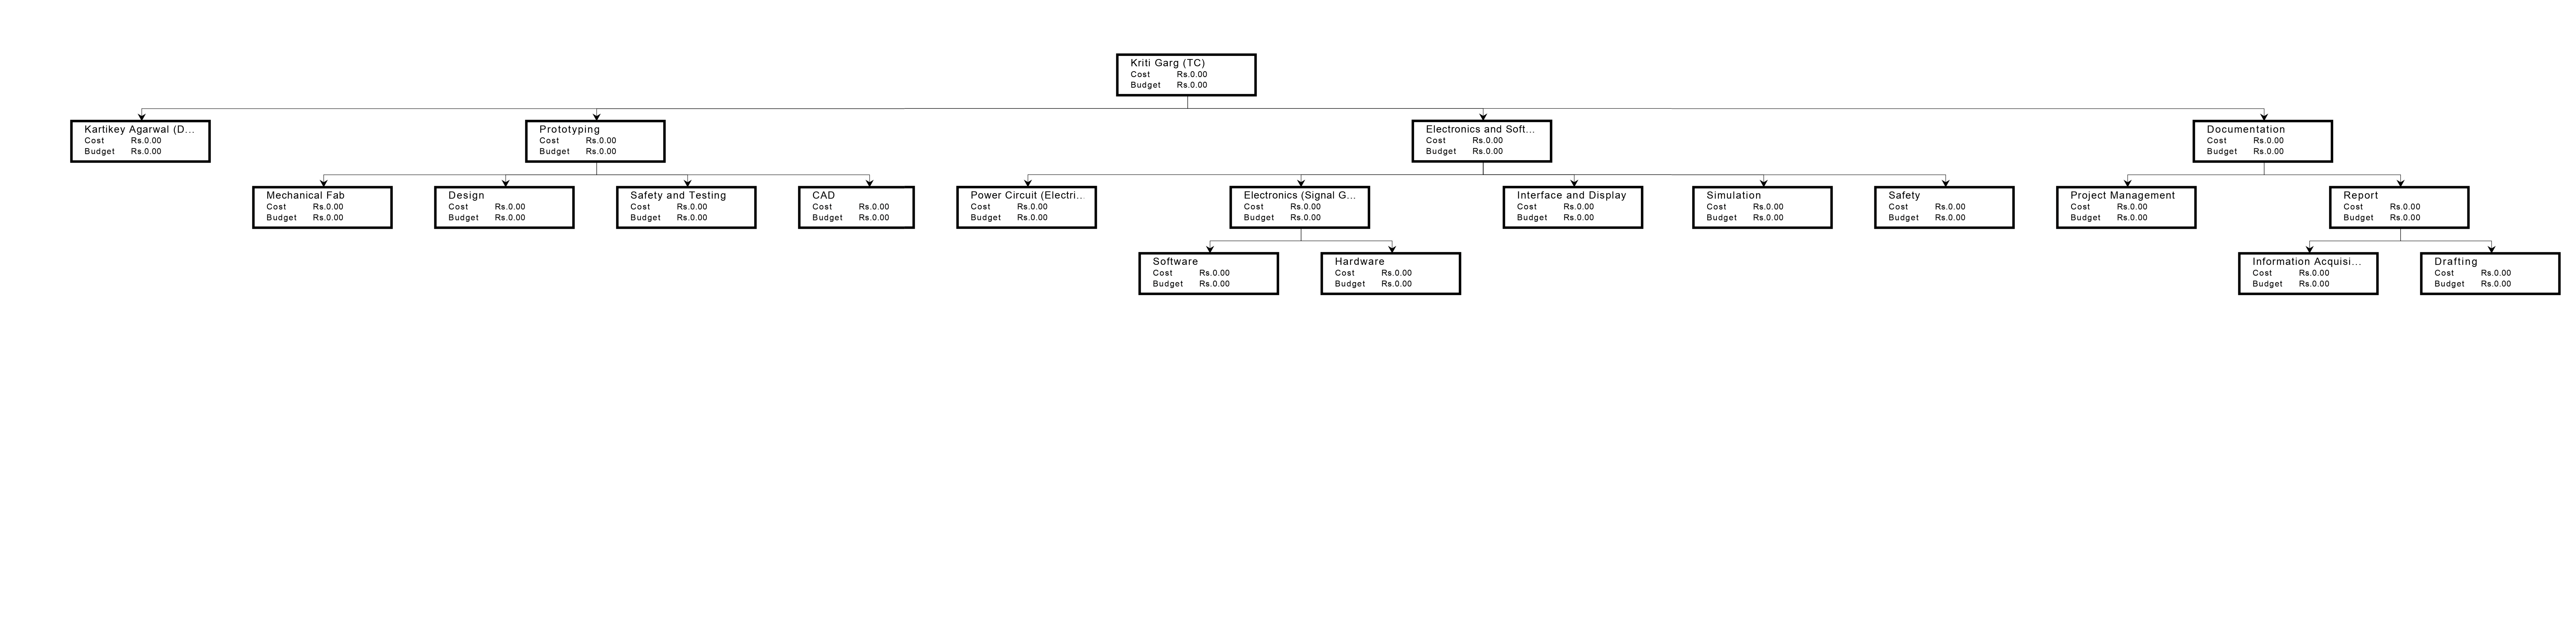
\includegraphics[width=1.36\textwidth]{ELP305_Monday_rbs_final_page-0003-imageonline.co-merged.jpg}}
    \caption{RBS Chart}
    \label{fig:RBS Chart}
\end{figure}

\clearpage

\begin{figure}[H]
    \centering
    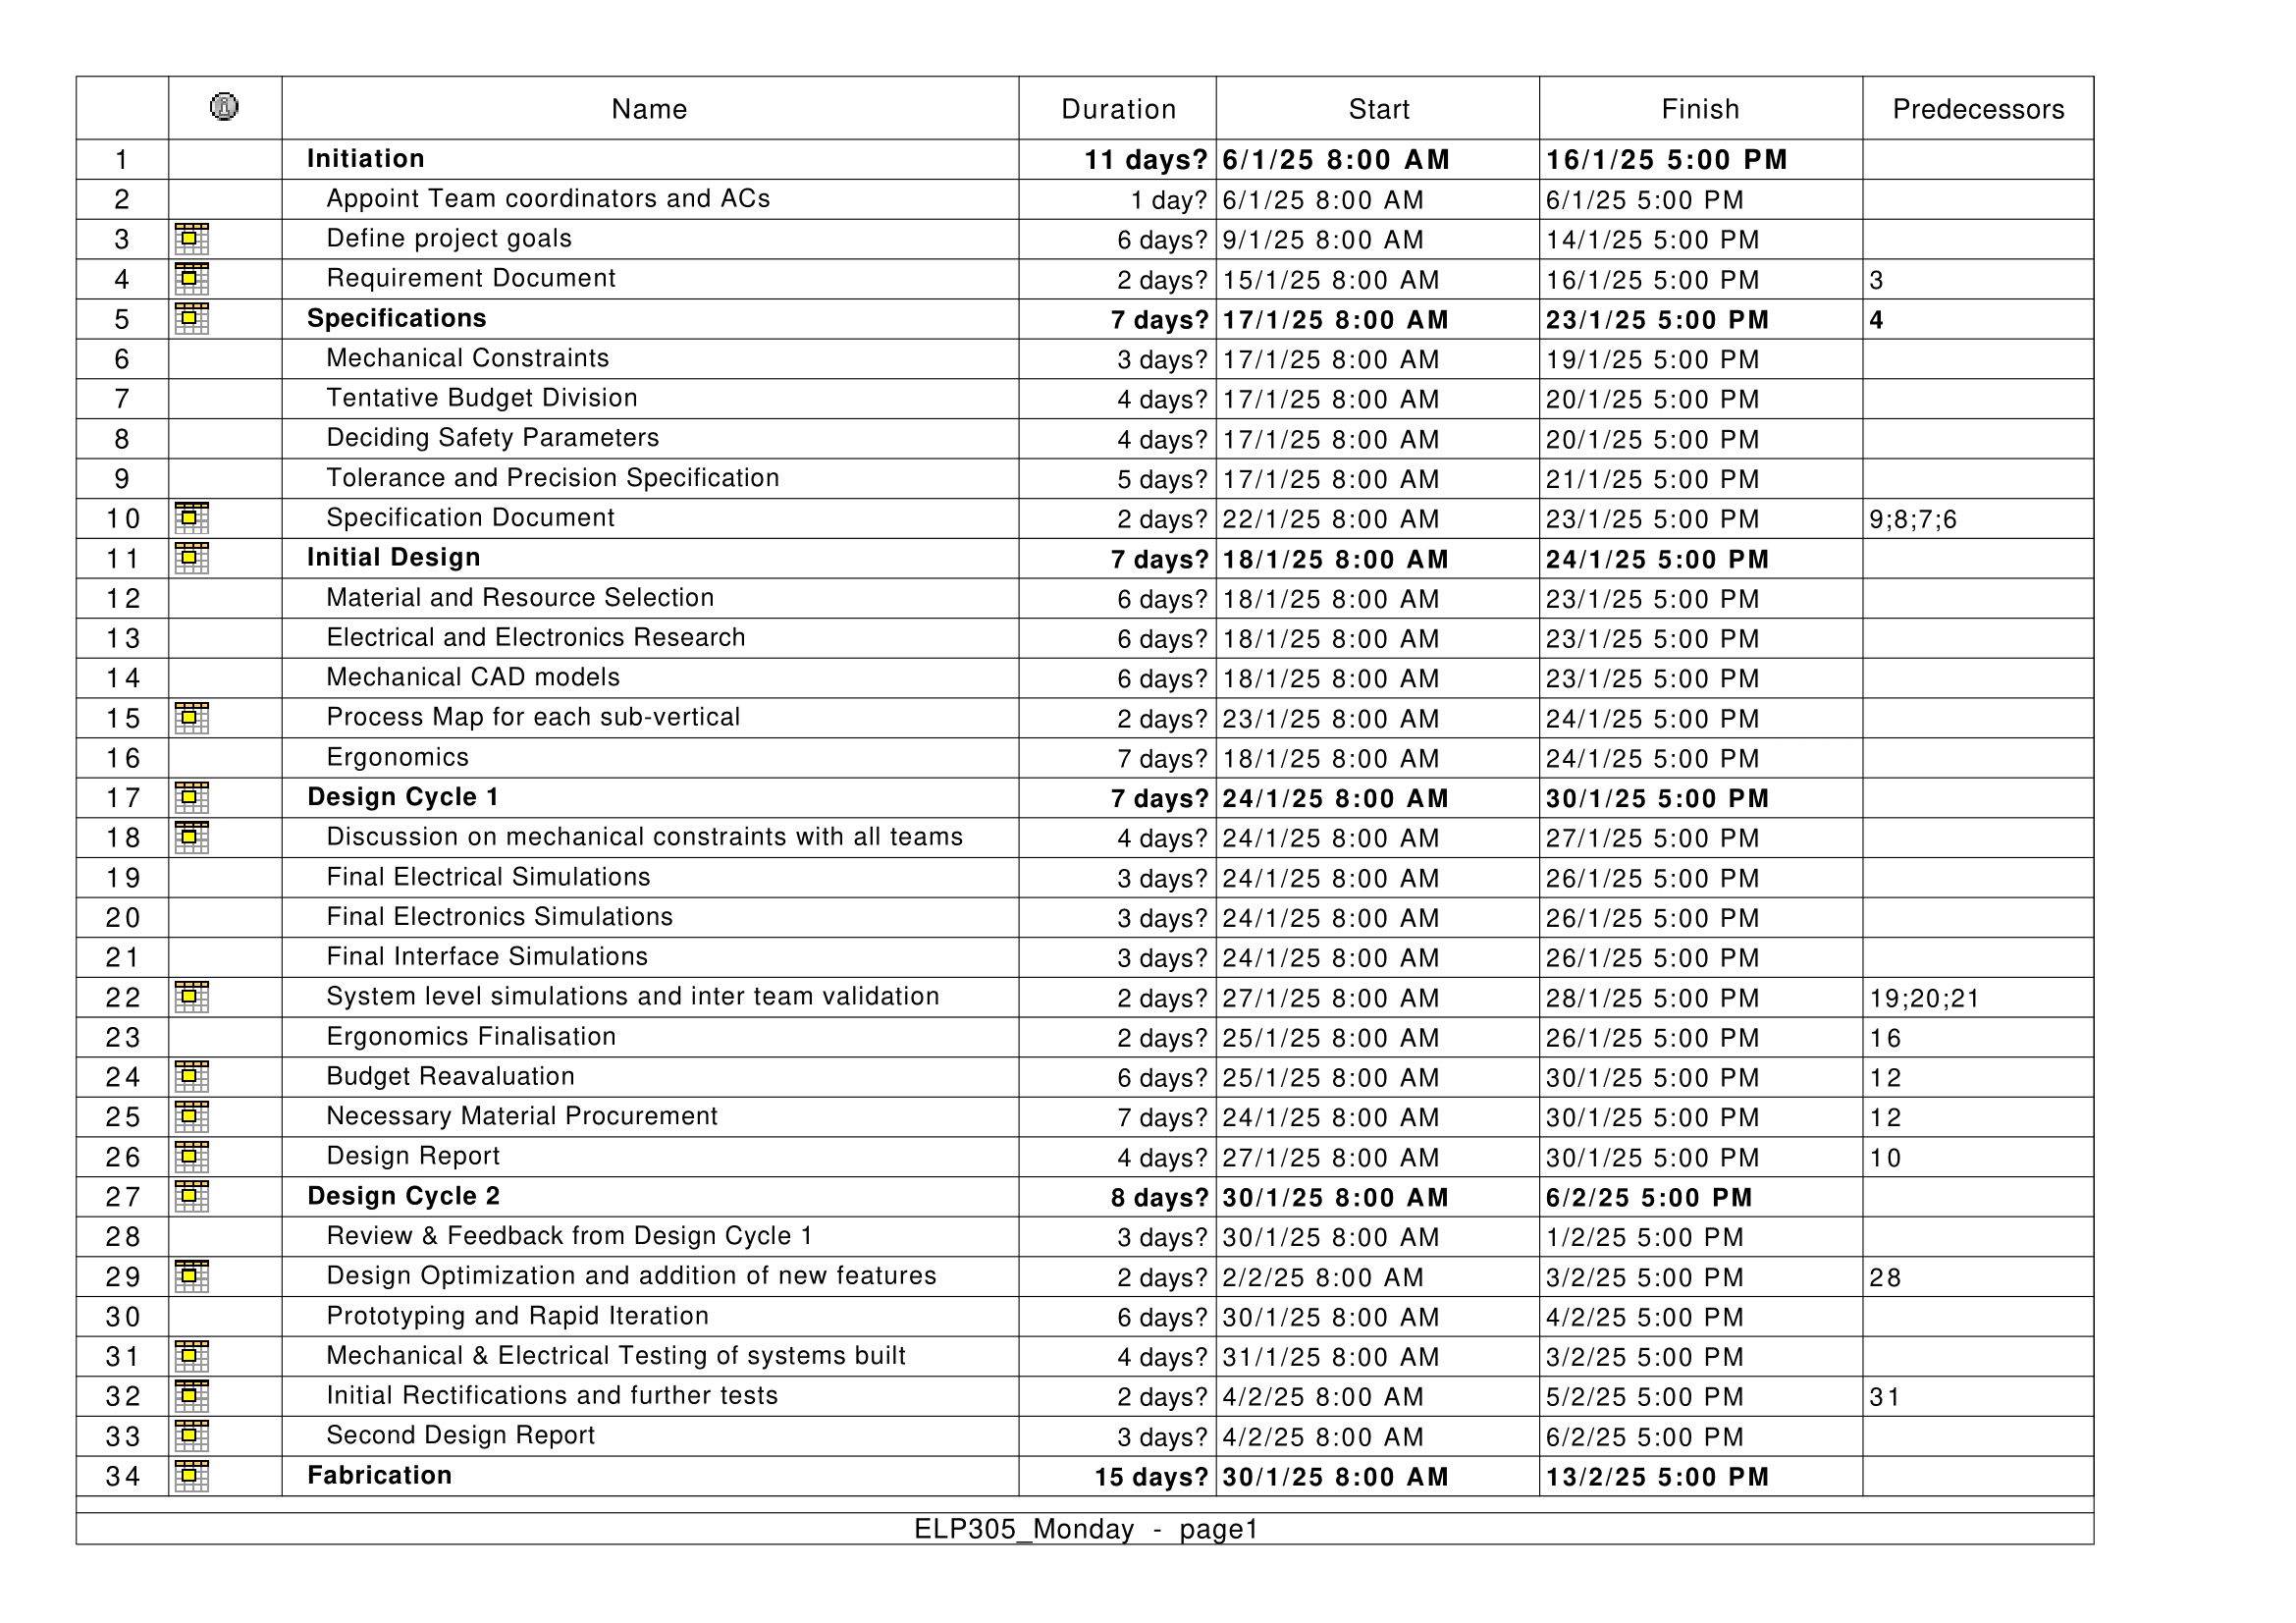
\includegraphics[width=1.2\textwidth]{gantt_new-1.png} % Replace with your file
    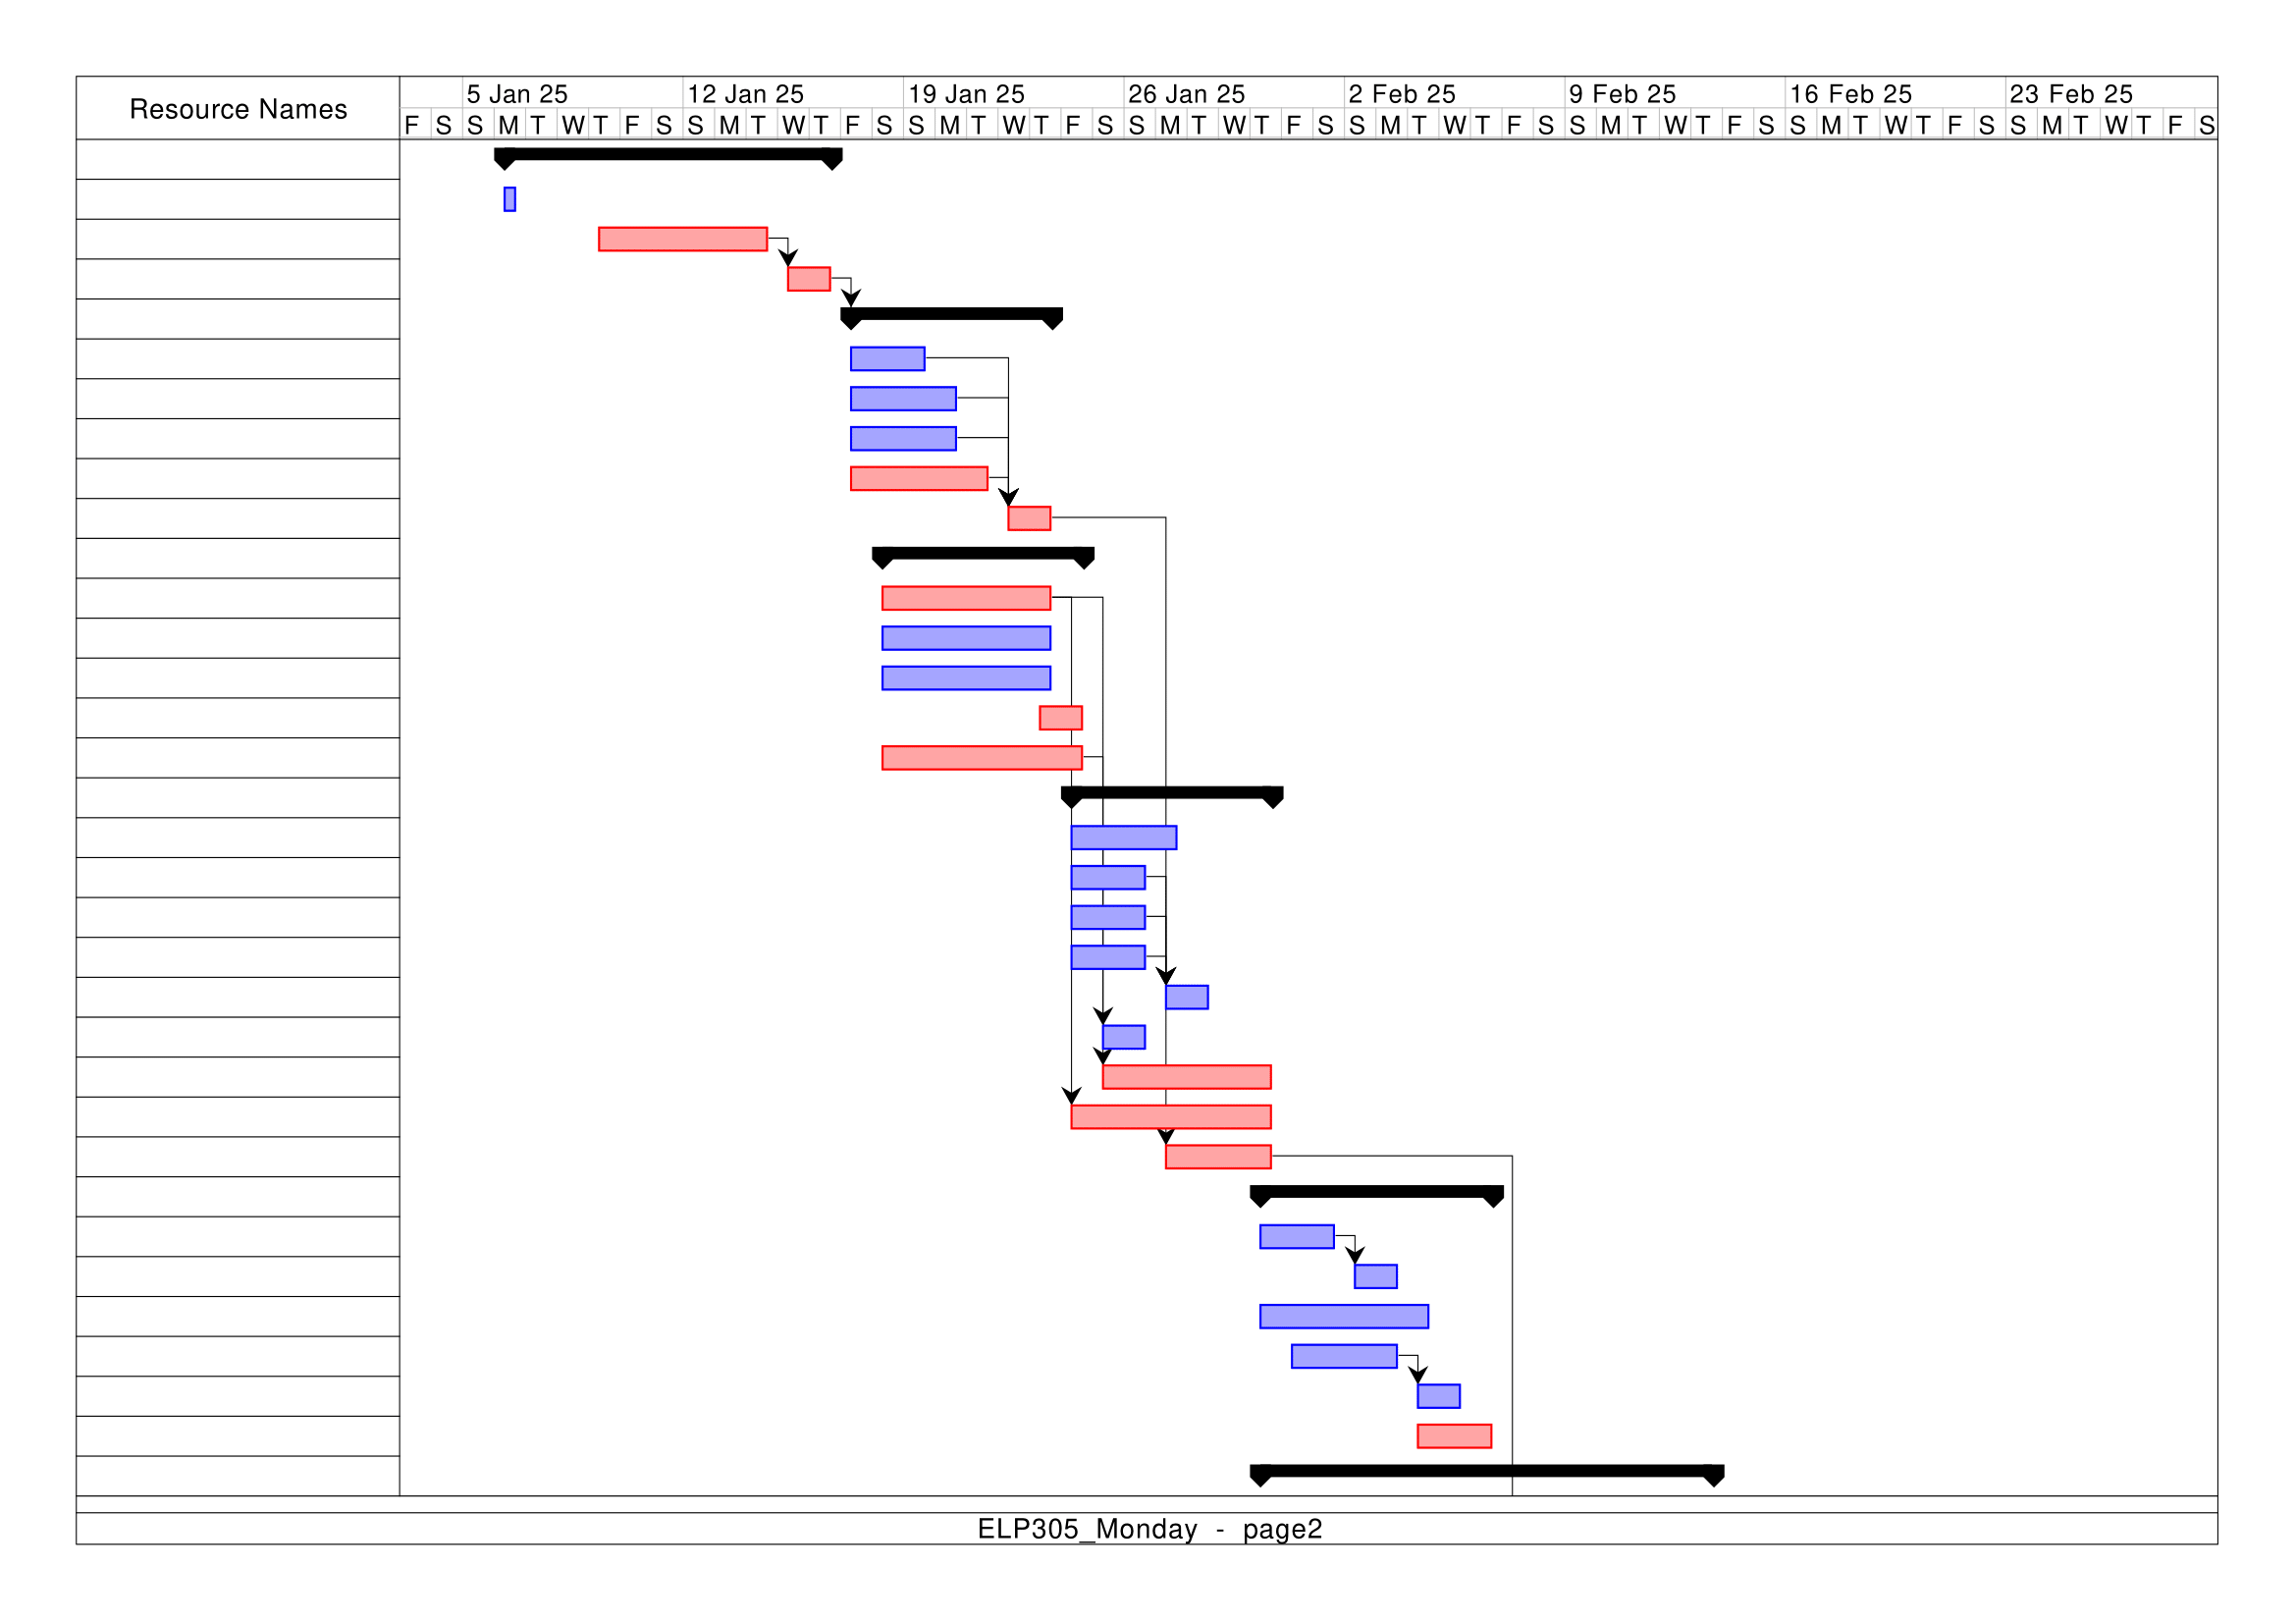
\includegraphics[width=1.2\textwidth]{gantt_new-2.png} % Replace with your file
    \caption{GANTT chart-I}
    
    \label{fig:GANTT CHART}
\end{figure}

\begin{figure}[H]
    \centering
    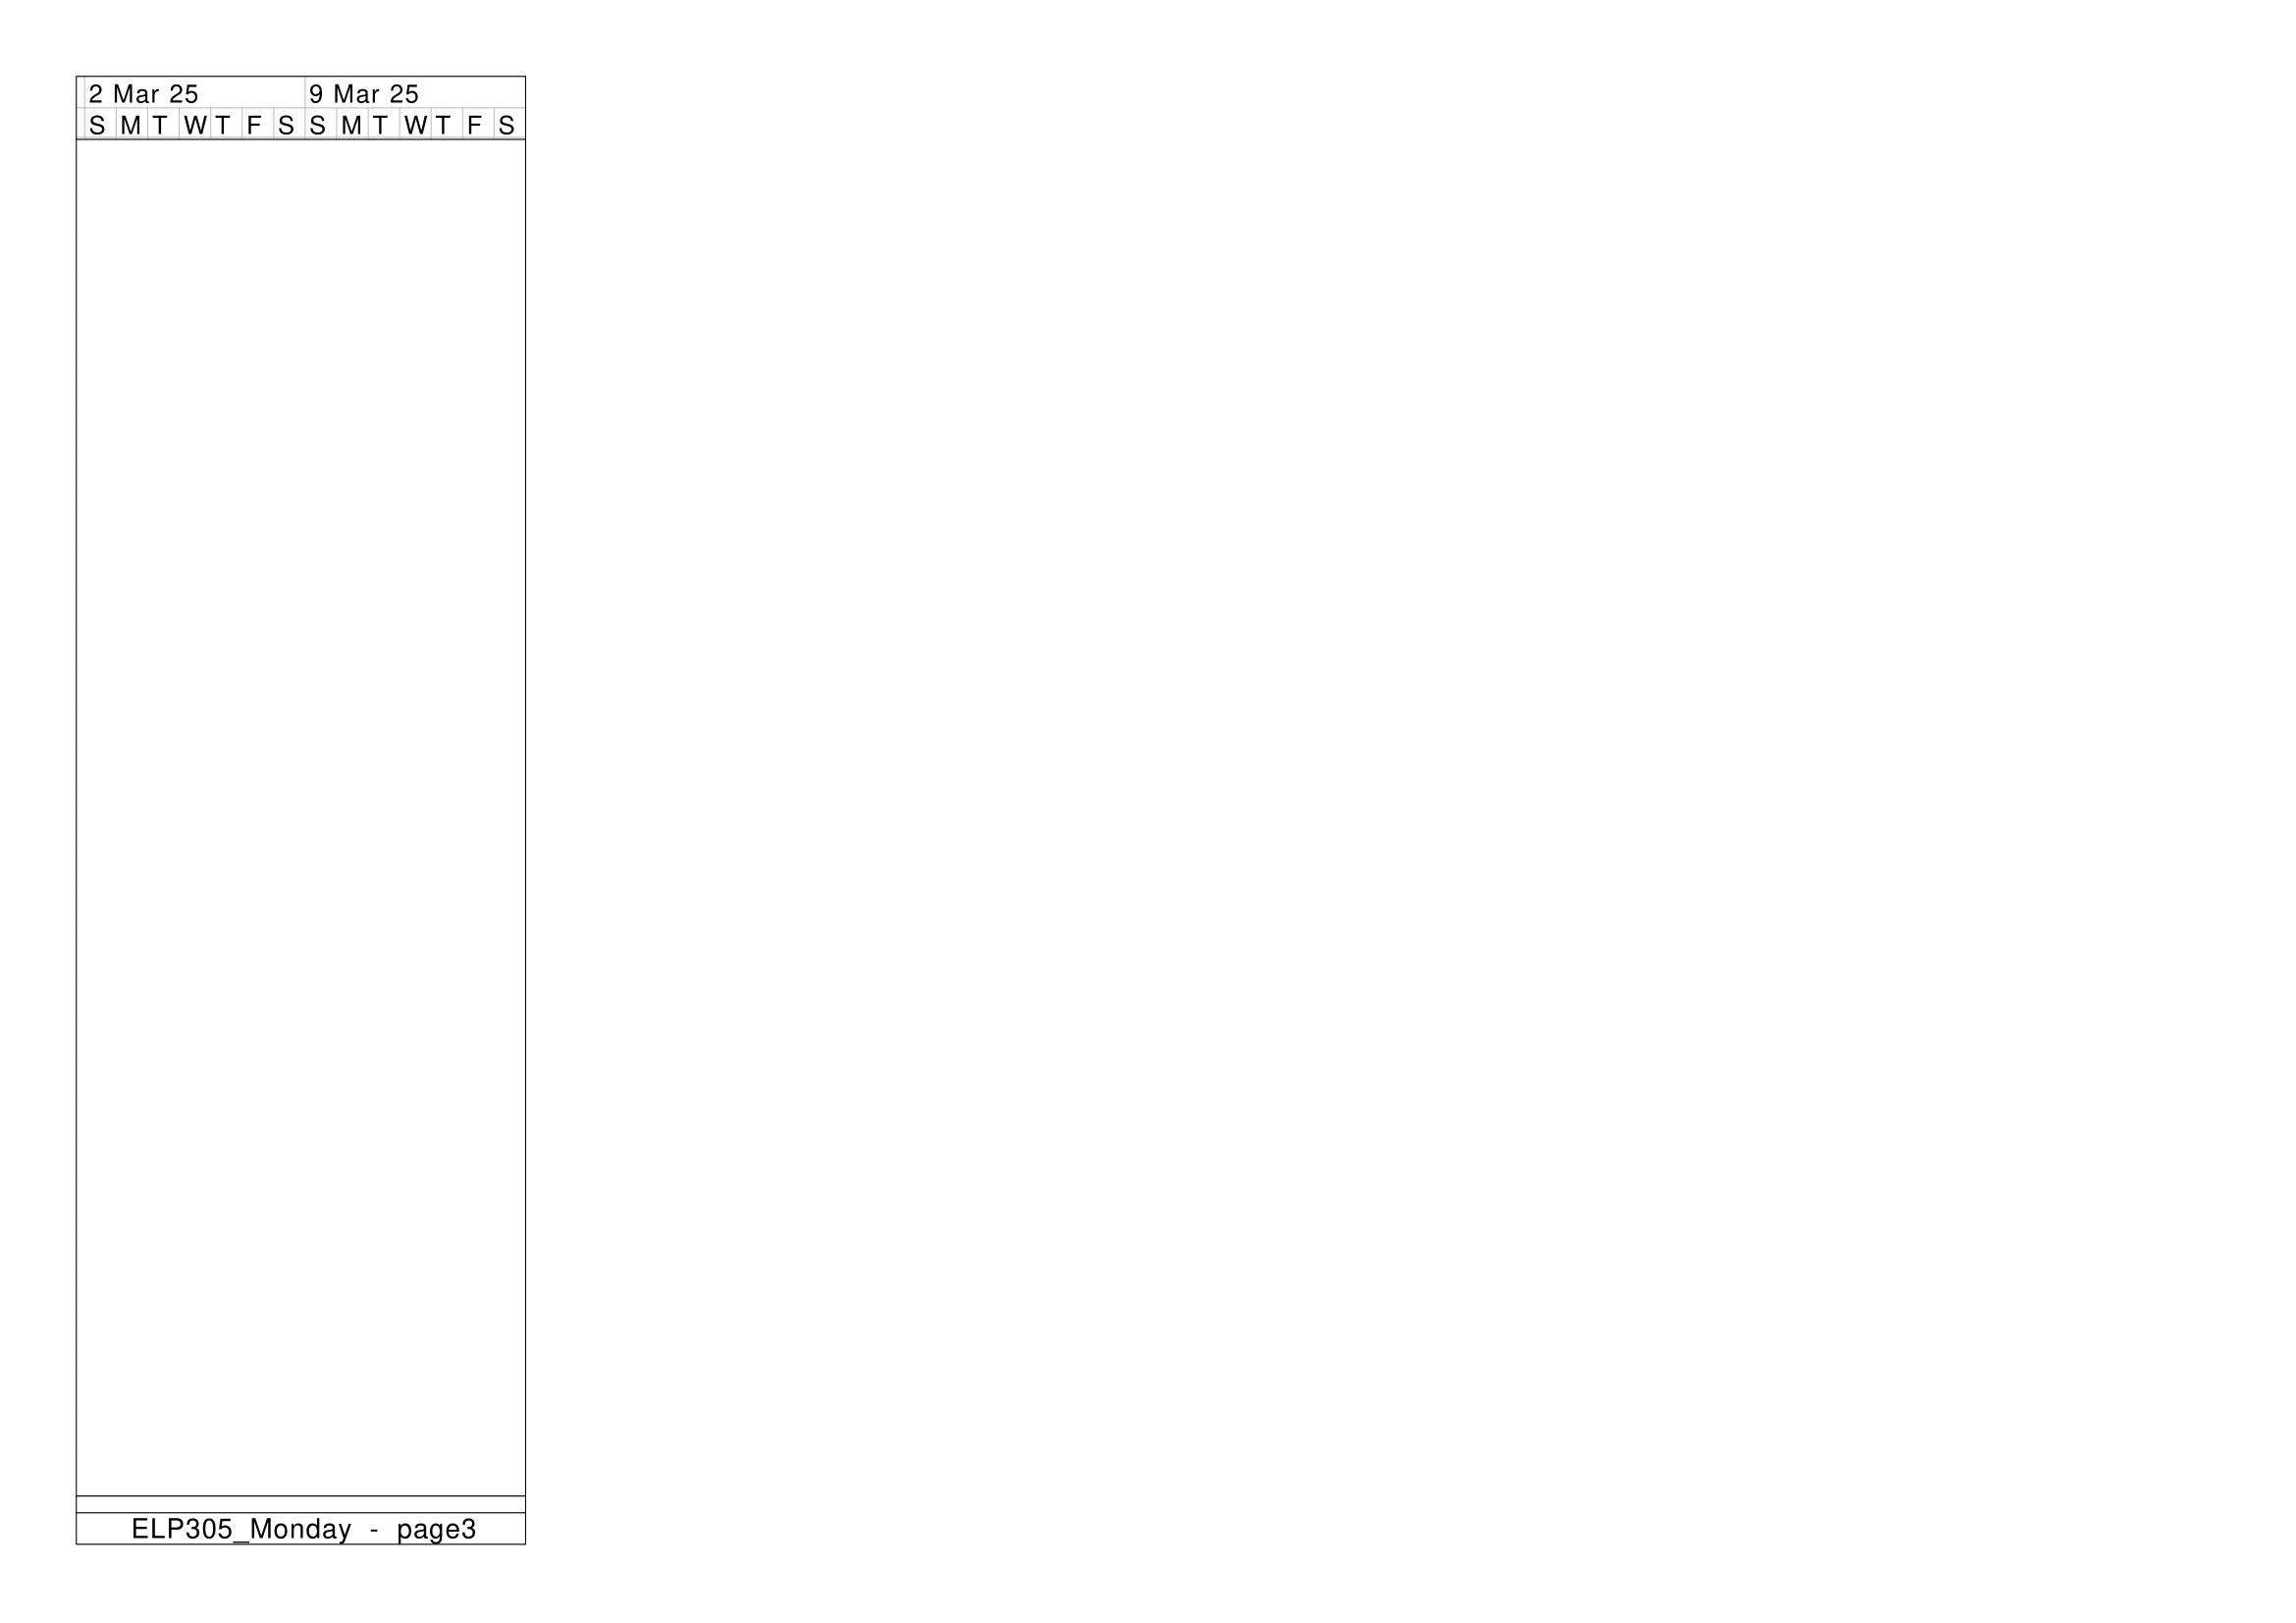
\includegraphics[width=1.2\textwidth]{gantt_new-3.png} % Replace with your file
    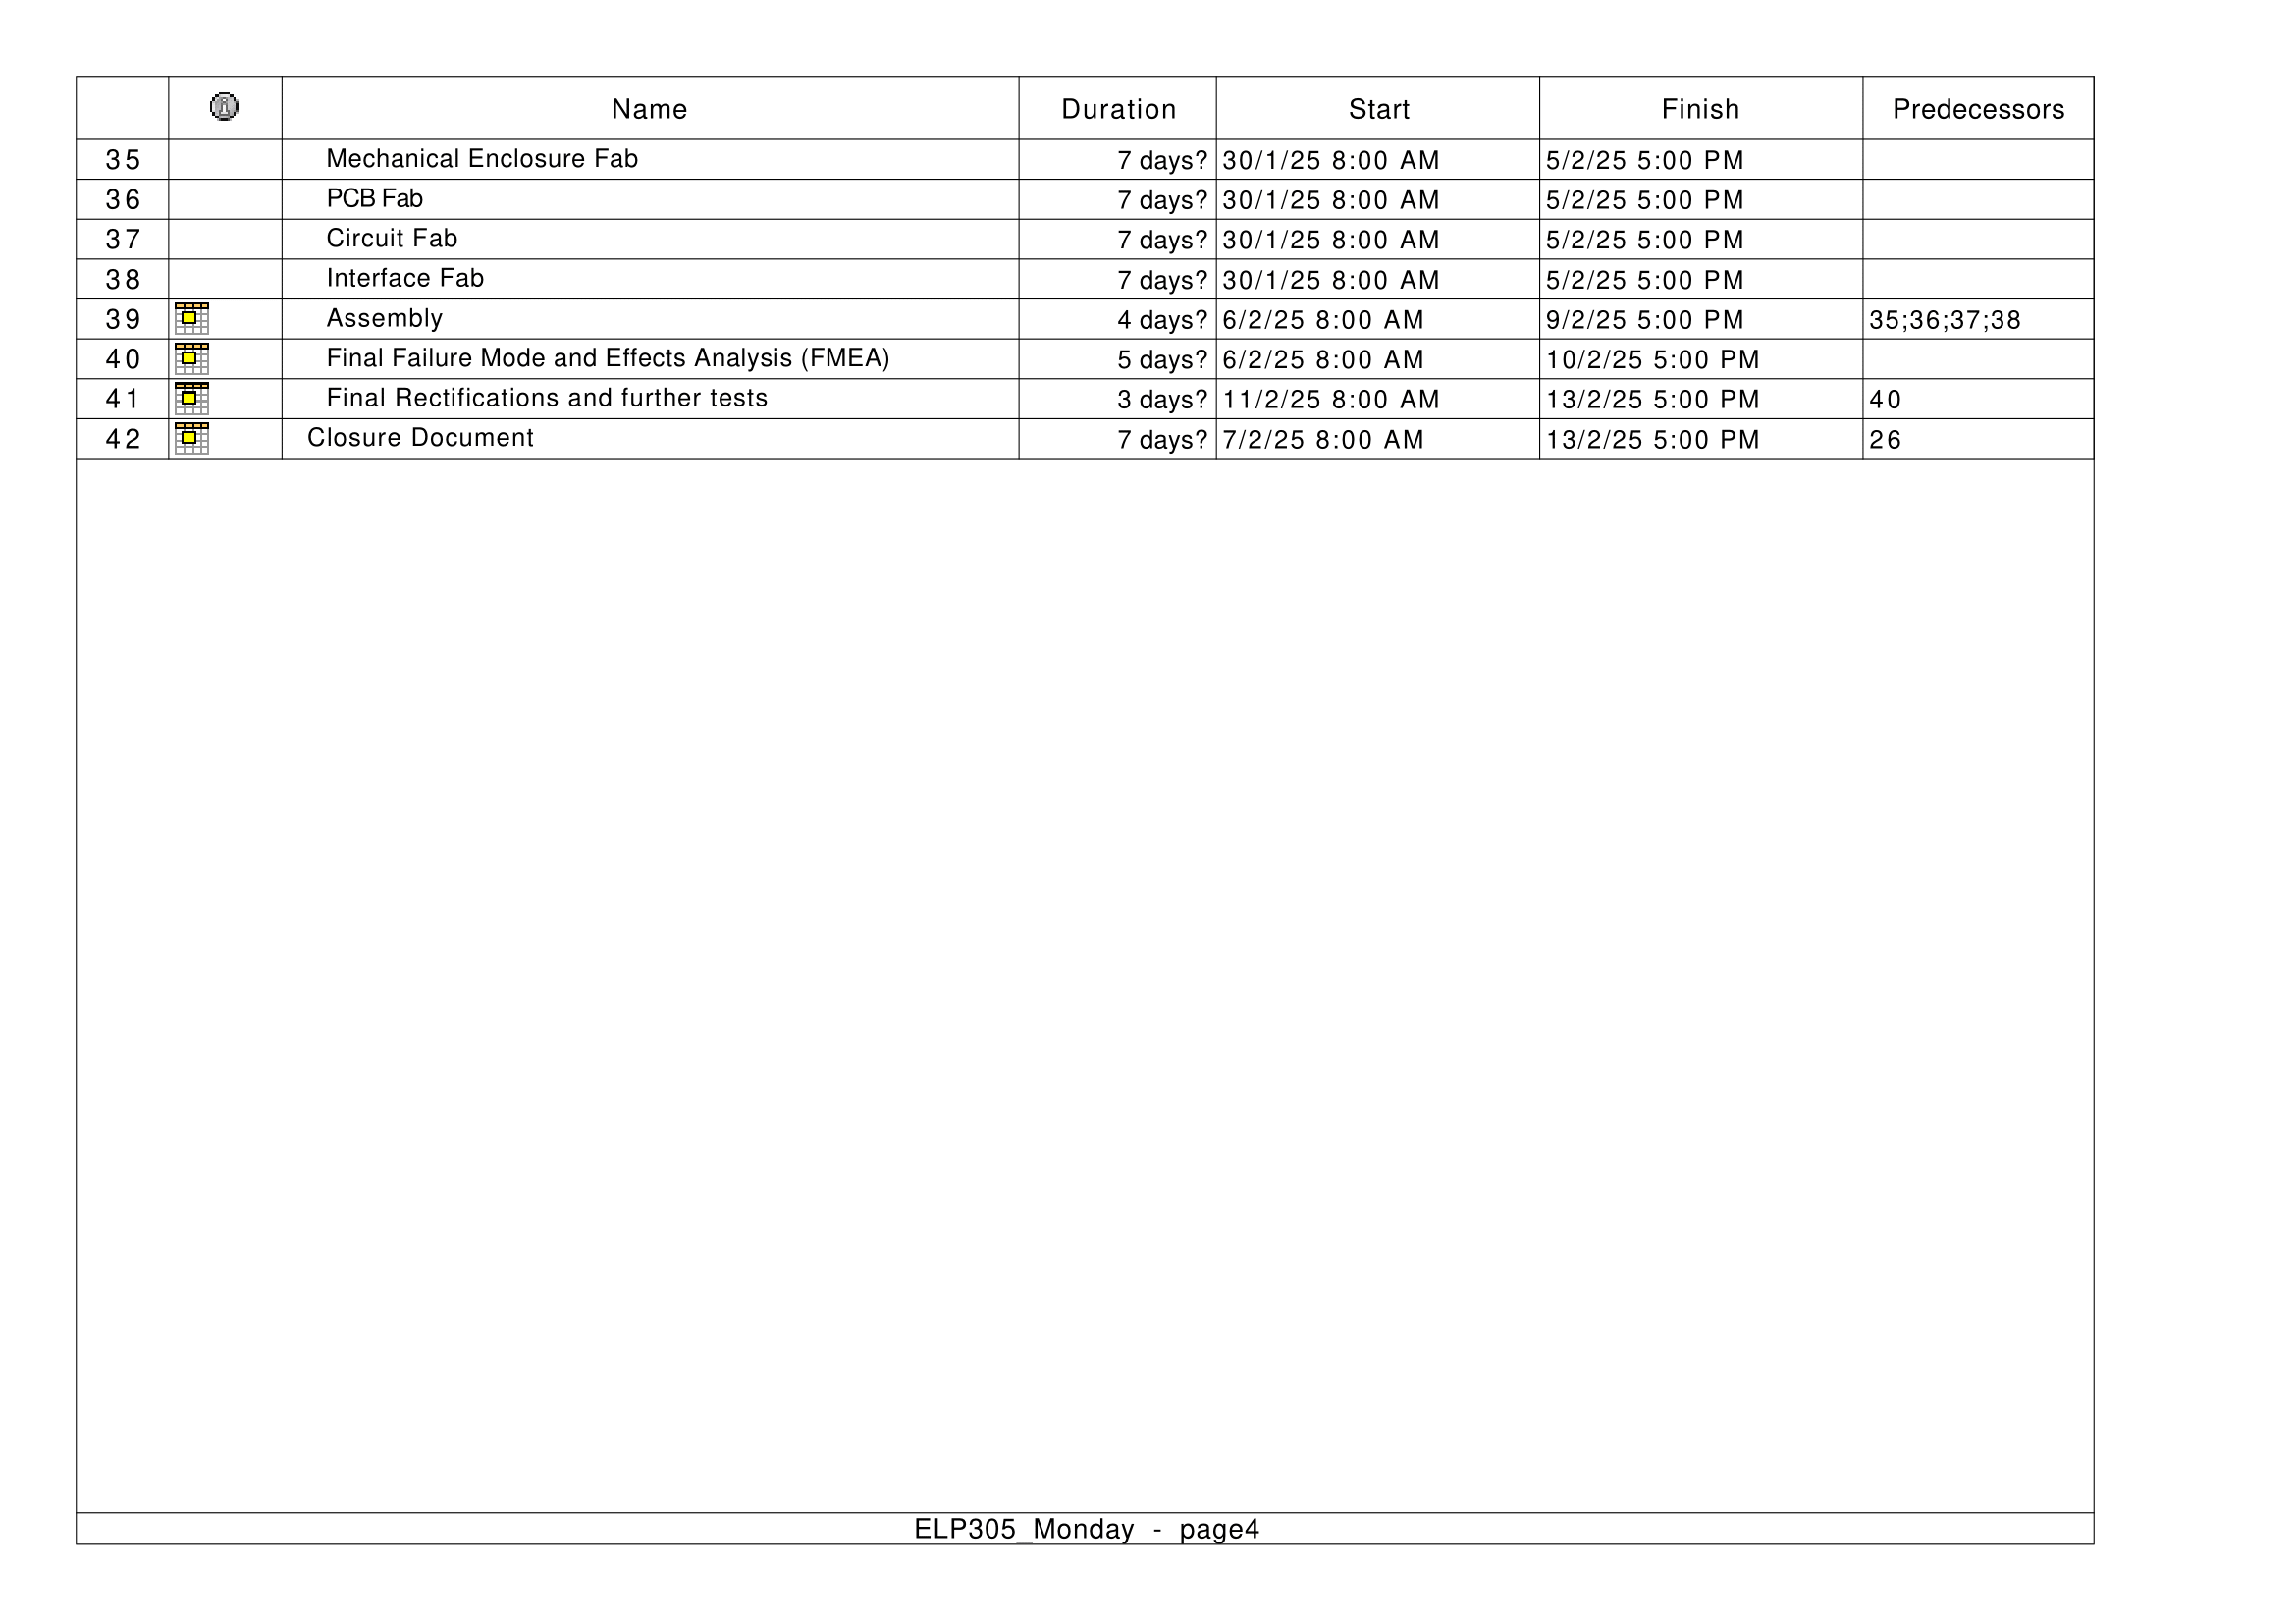
\includegraphics[width=1.2\textwidth]{gantt_new-4.png} % Replace with your file
    
    \caption{GANTT chart-II}
    
    \label{fig:GANTT CHART}
\end{figure}

\begin{figure}[H]
    \centering
    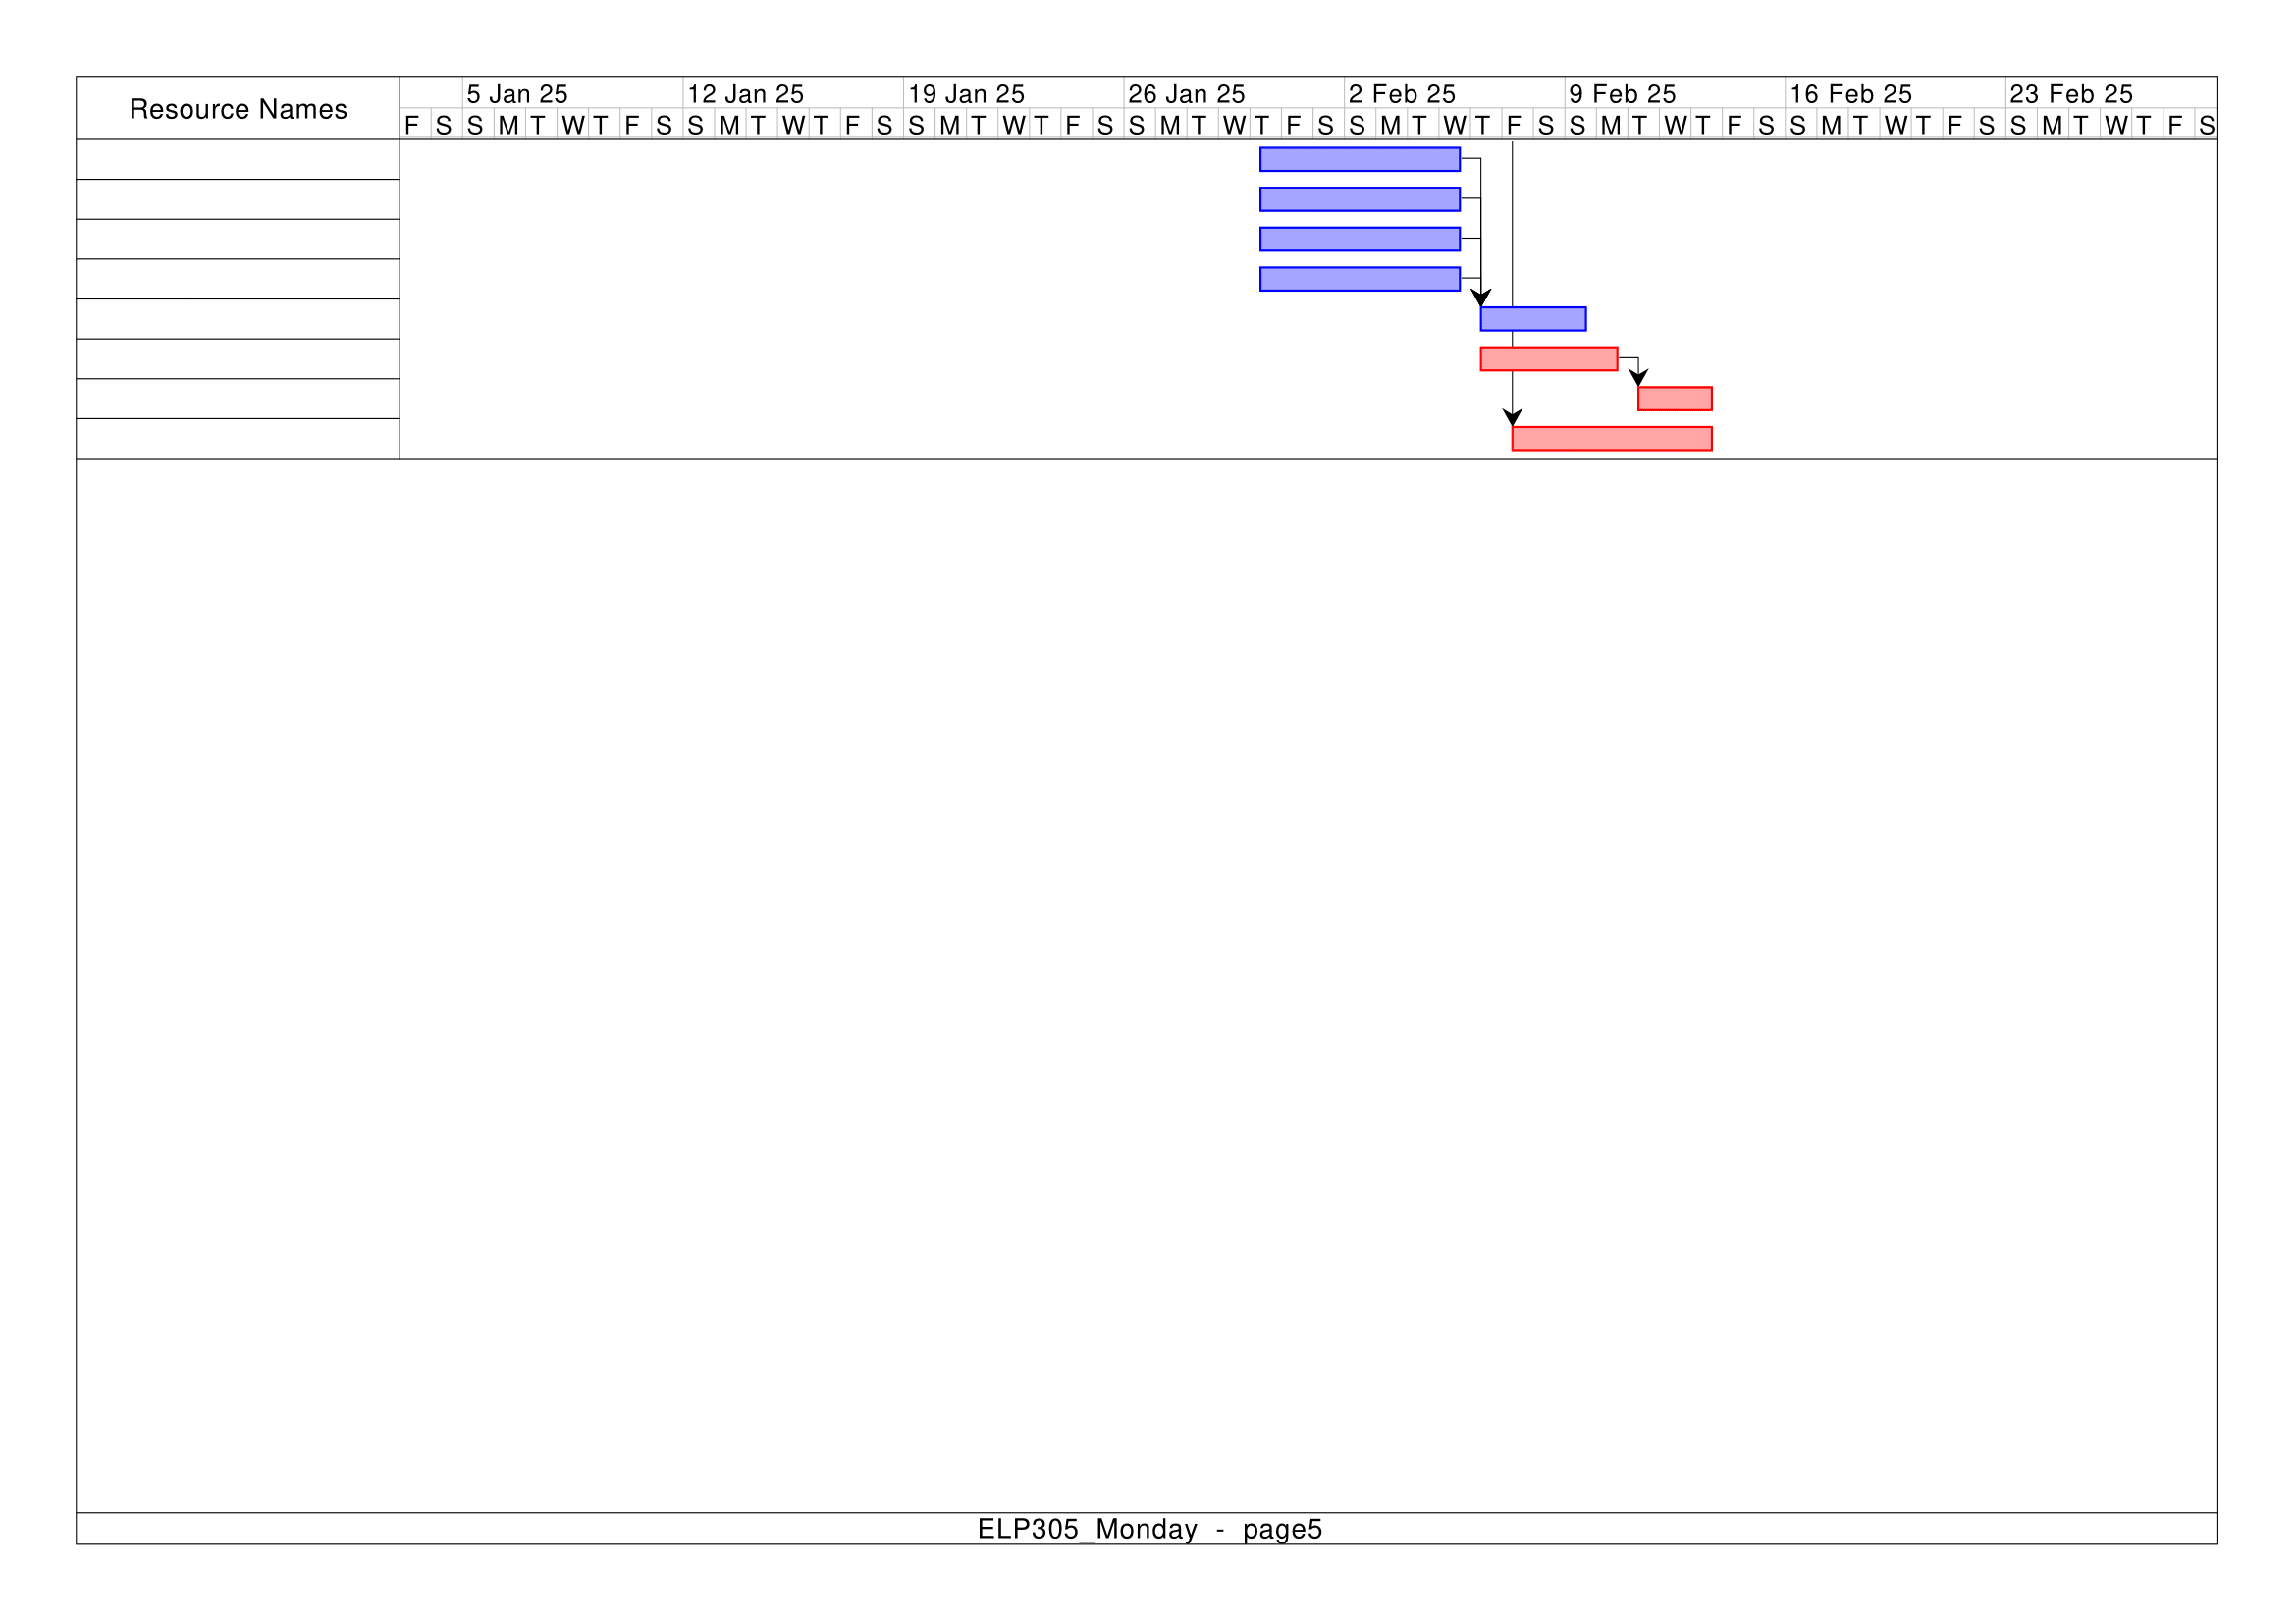
\includegraphics[width=1.2\textwidth]{gantt_new-5.png} % Replace with your file
    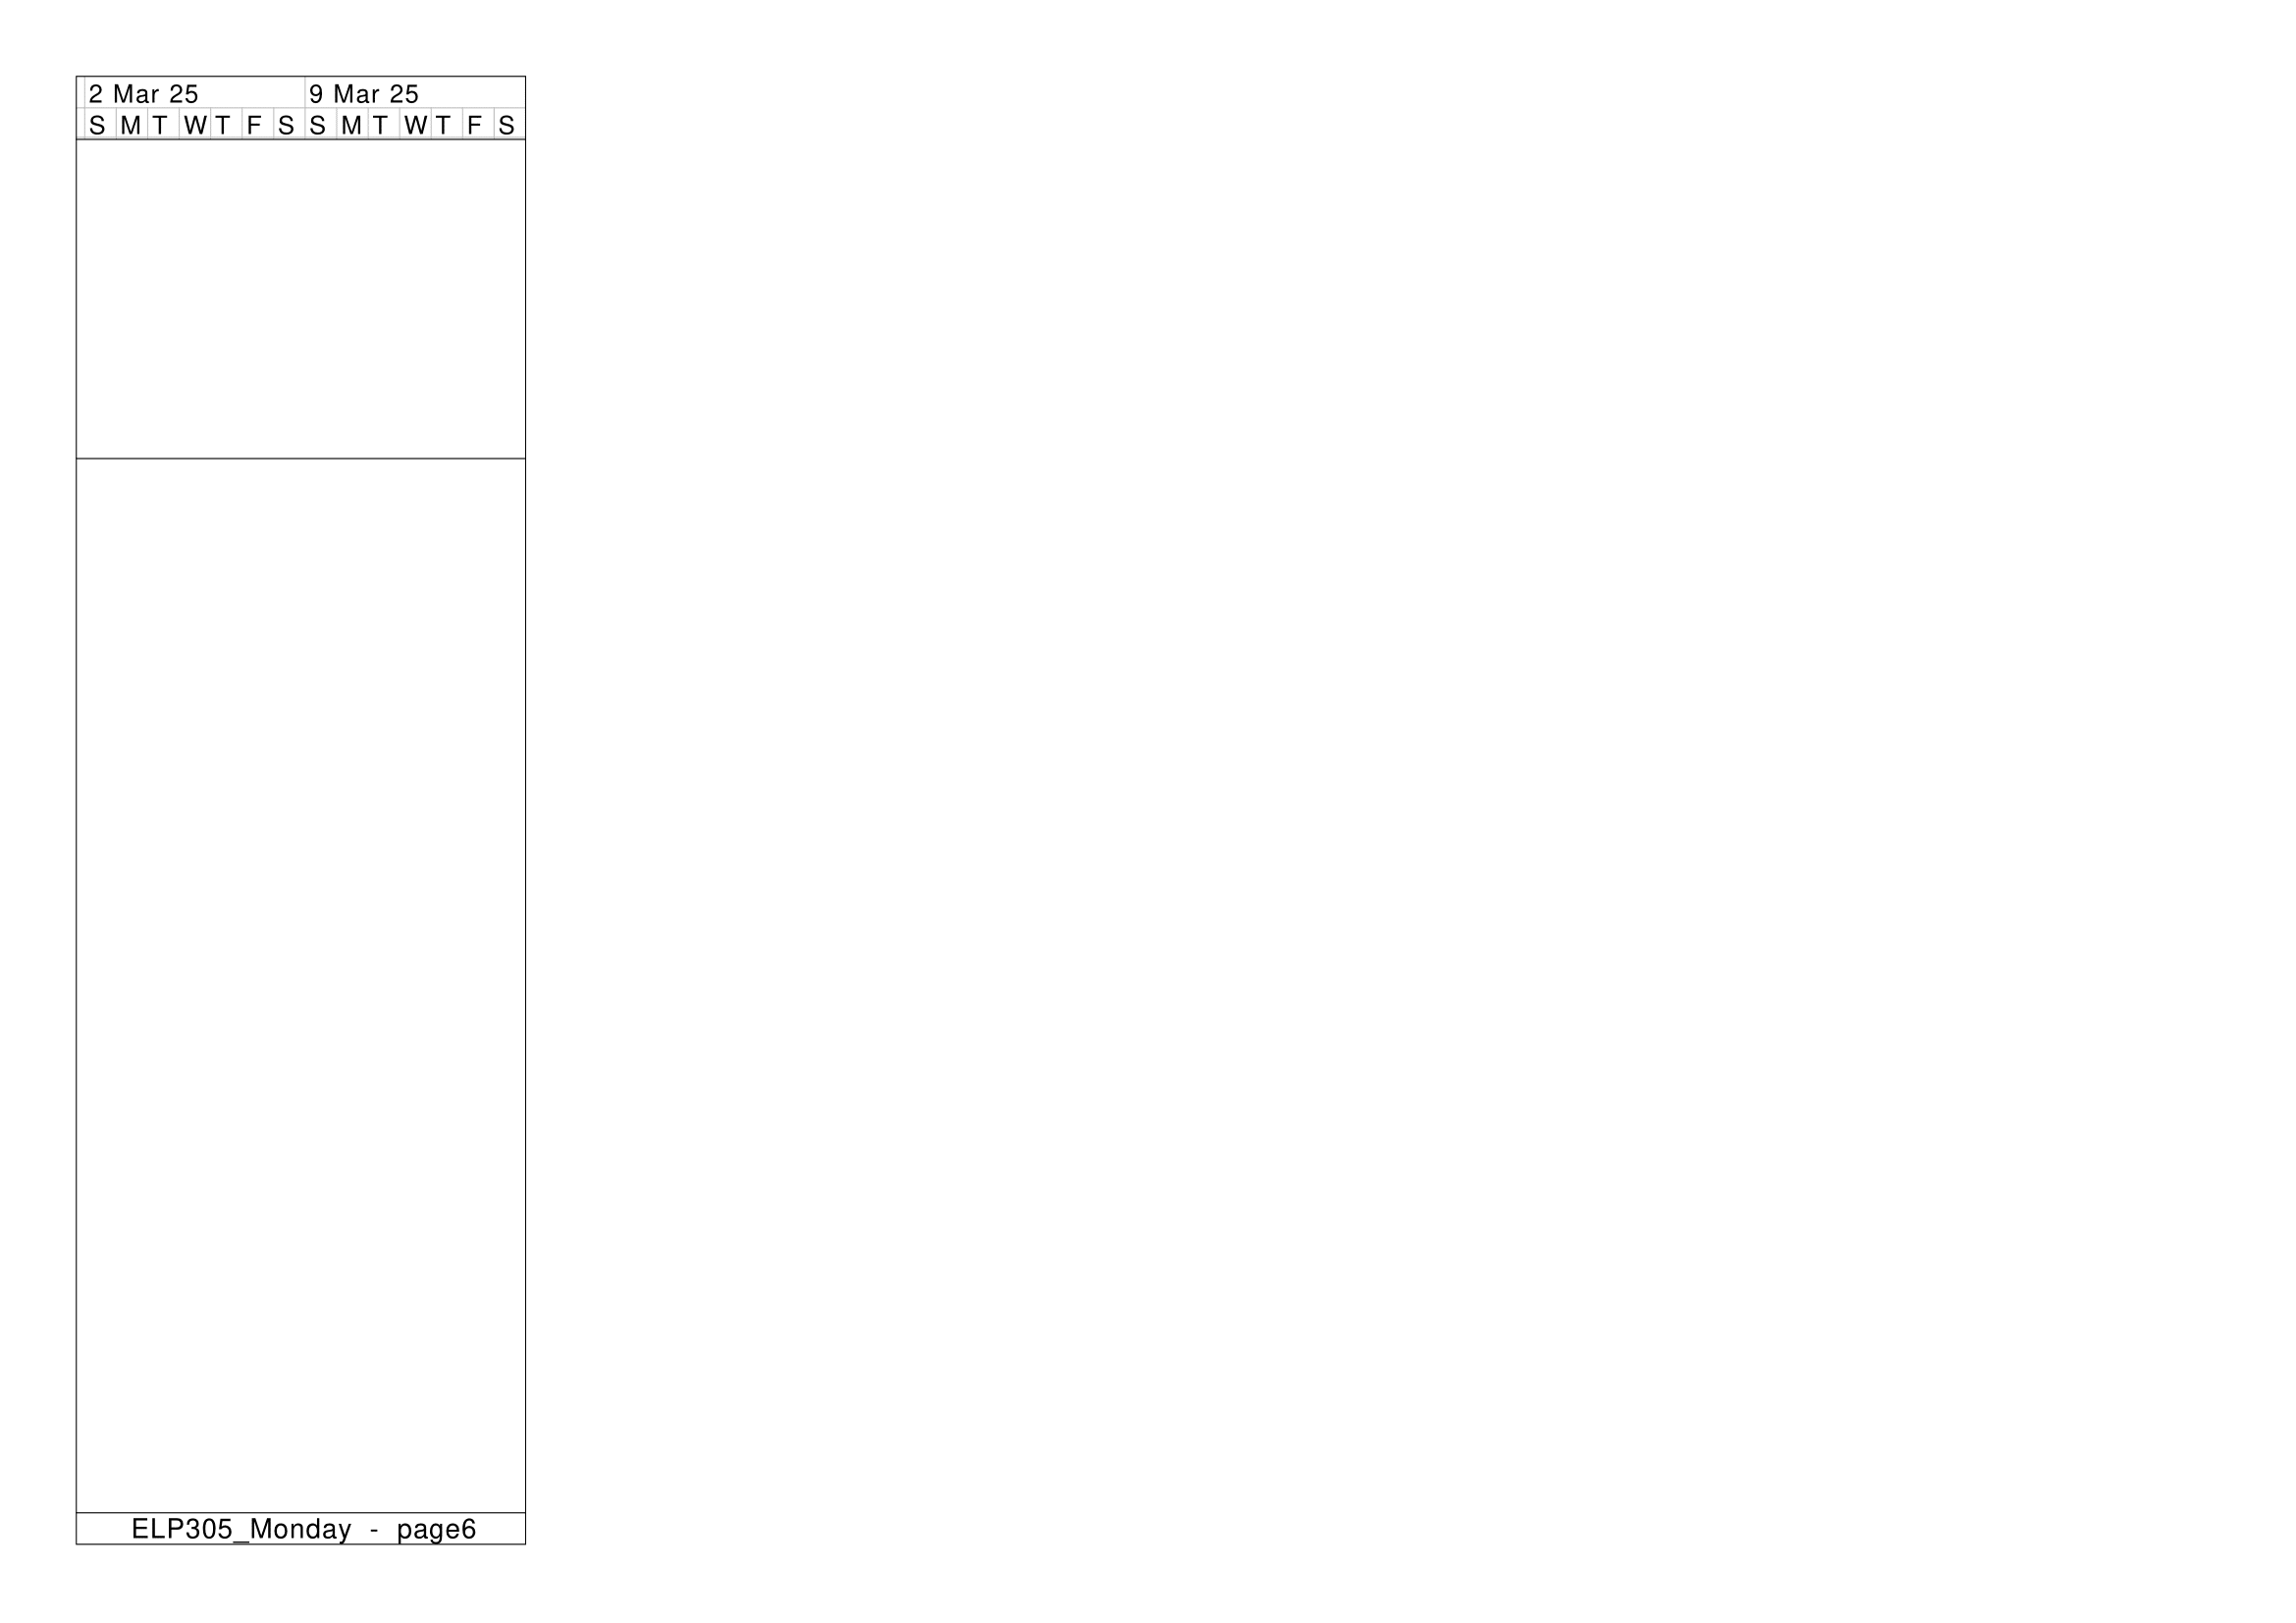
\includegraphics[width=1.2\textwidth]{gantt_new-6.png} % Replace with your file
    
    \caption{GANTT chart-III}
    
    \label{fig:GANTT CHART}
\end{figure}

\begin{figure}[H]
    \centering
    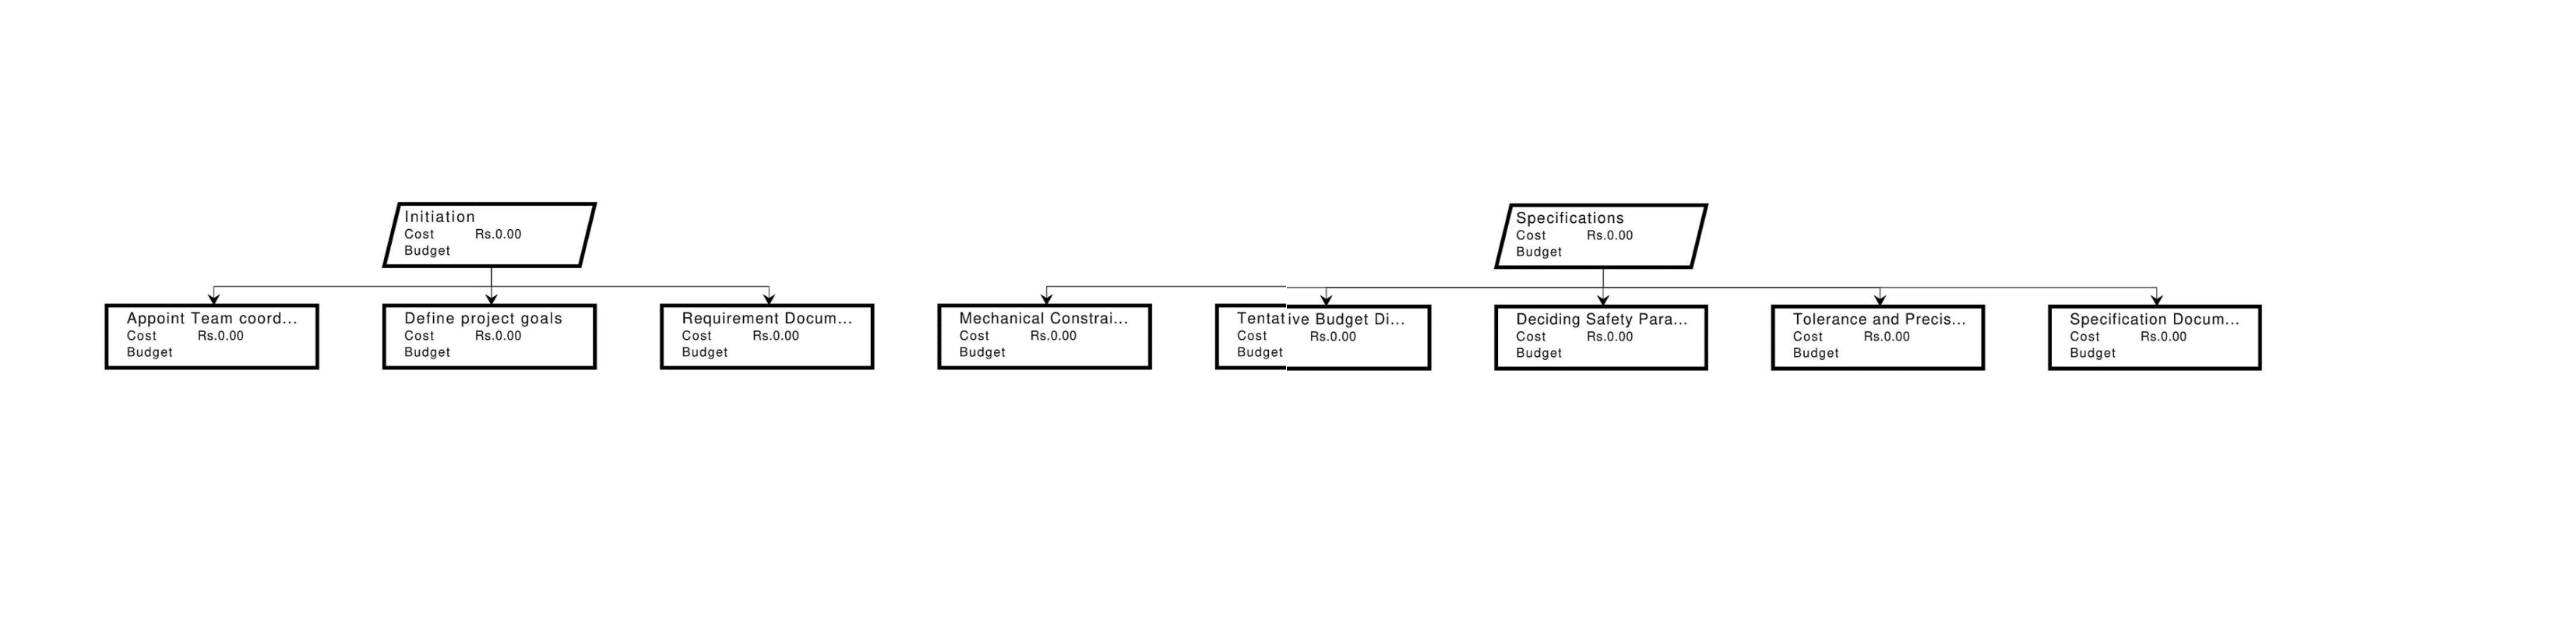
\includegraphics[width=1\textwidth]{WBS-1.png} % Replace with your file
    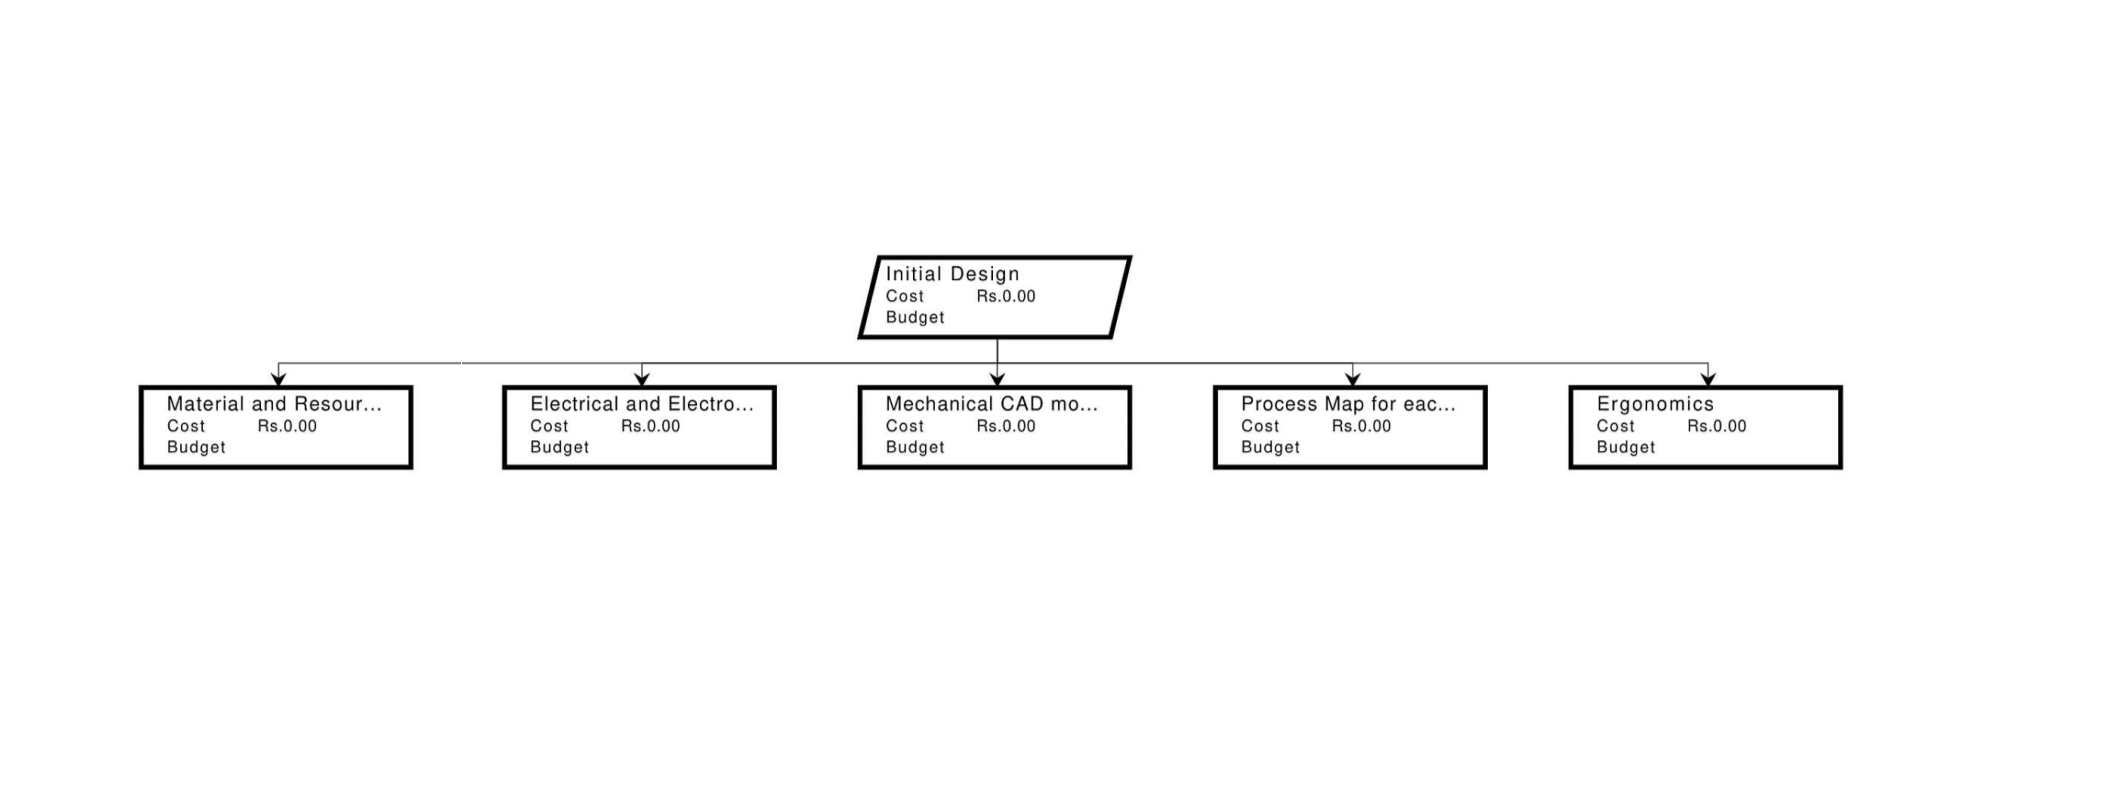
\includegraphics[width=1\textwidth]{WBS-2.png} % Replace with your file
    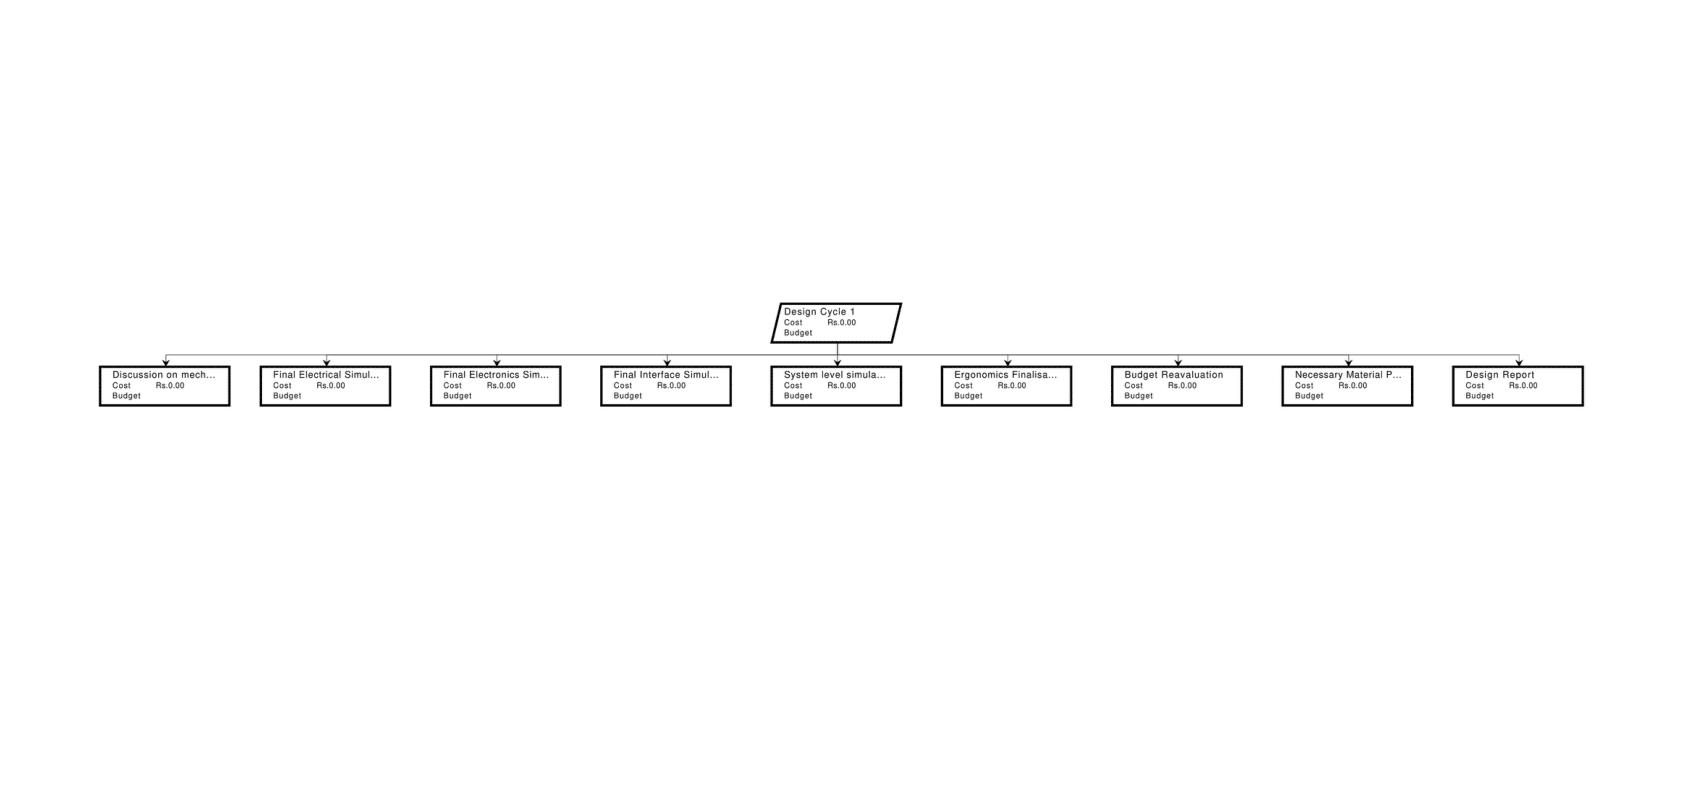
\includegraphics[width=1\textwidth]{WBS-3.png} % Replace with your file
    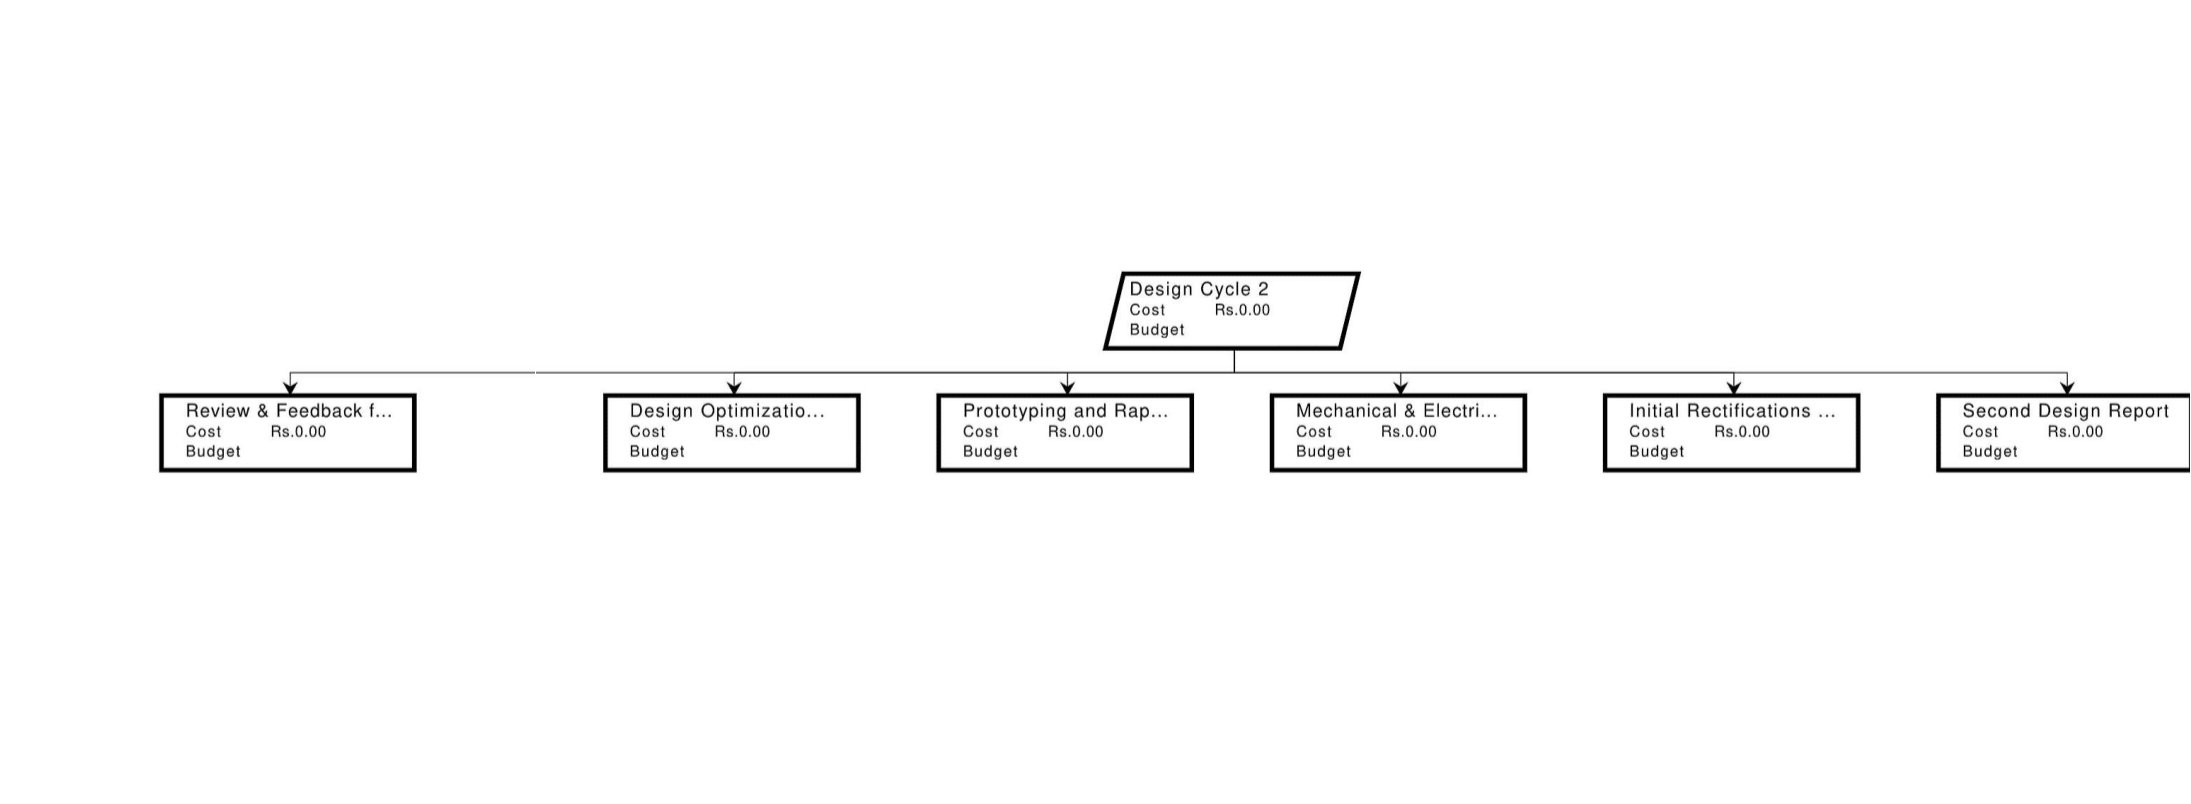
\includegraphics[width=1\textwidth]{WBS-4.png} % Replace with your file
    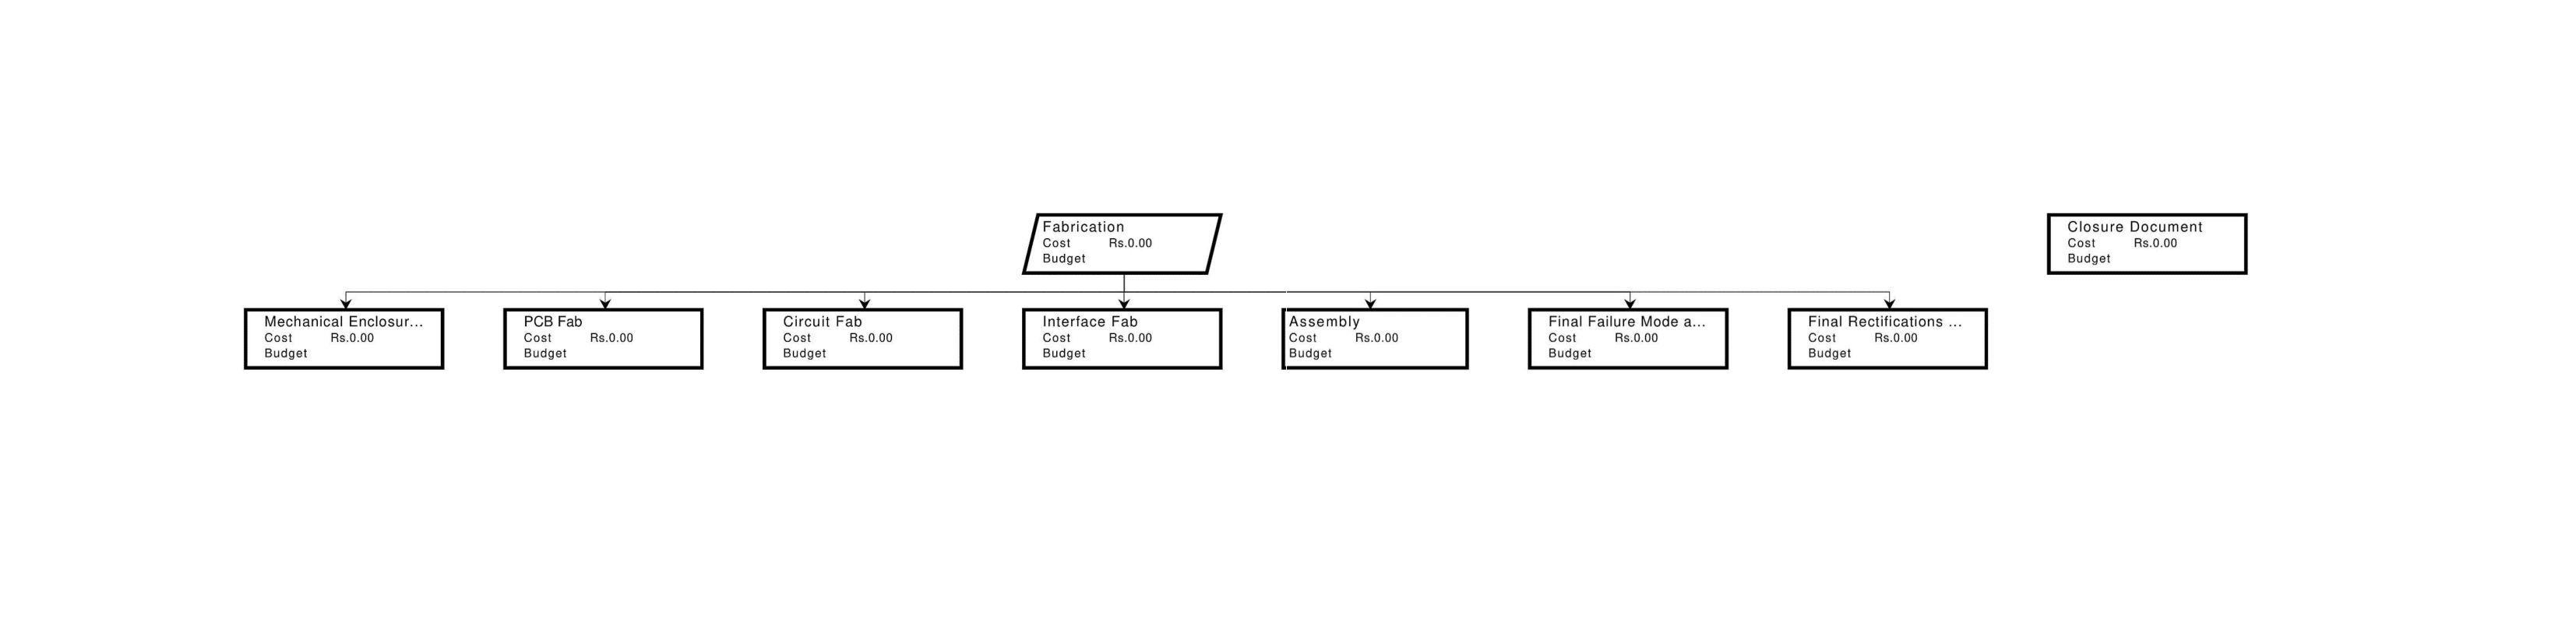
\includegraphics[width=1\textwidth]{WBS-5.png} % Replace with your file
    \caption{WBS Chart}
    
    \label{fig:GANTT CHART}
\end{figure}

\newpage

\begin{figure}[H]
    \centering
    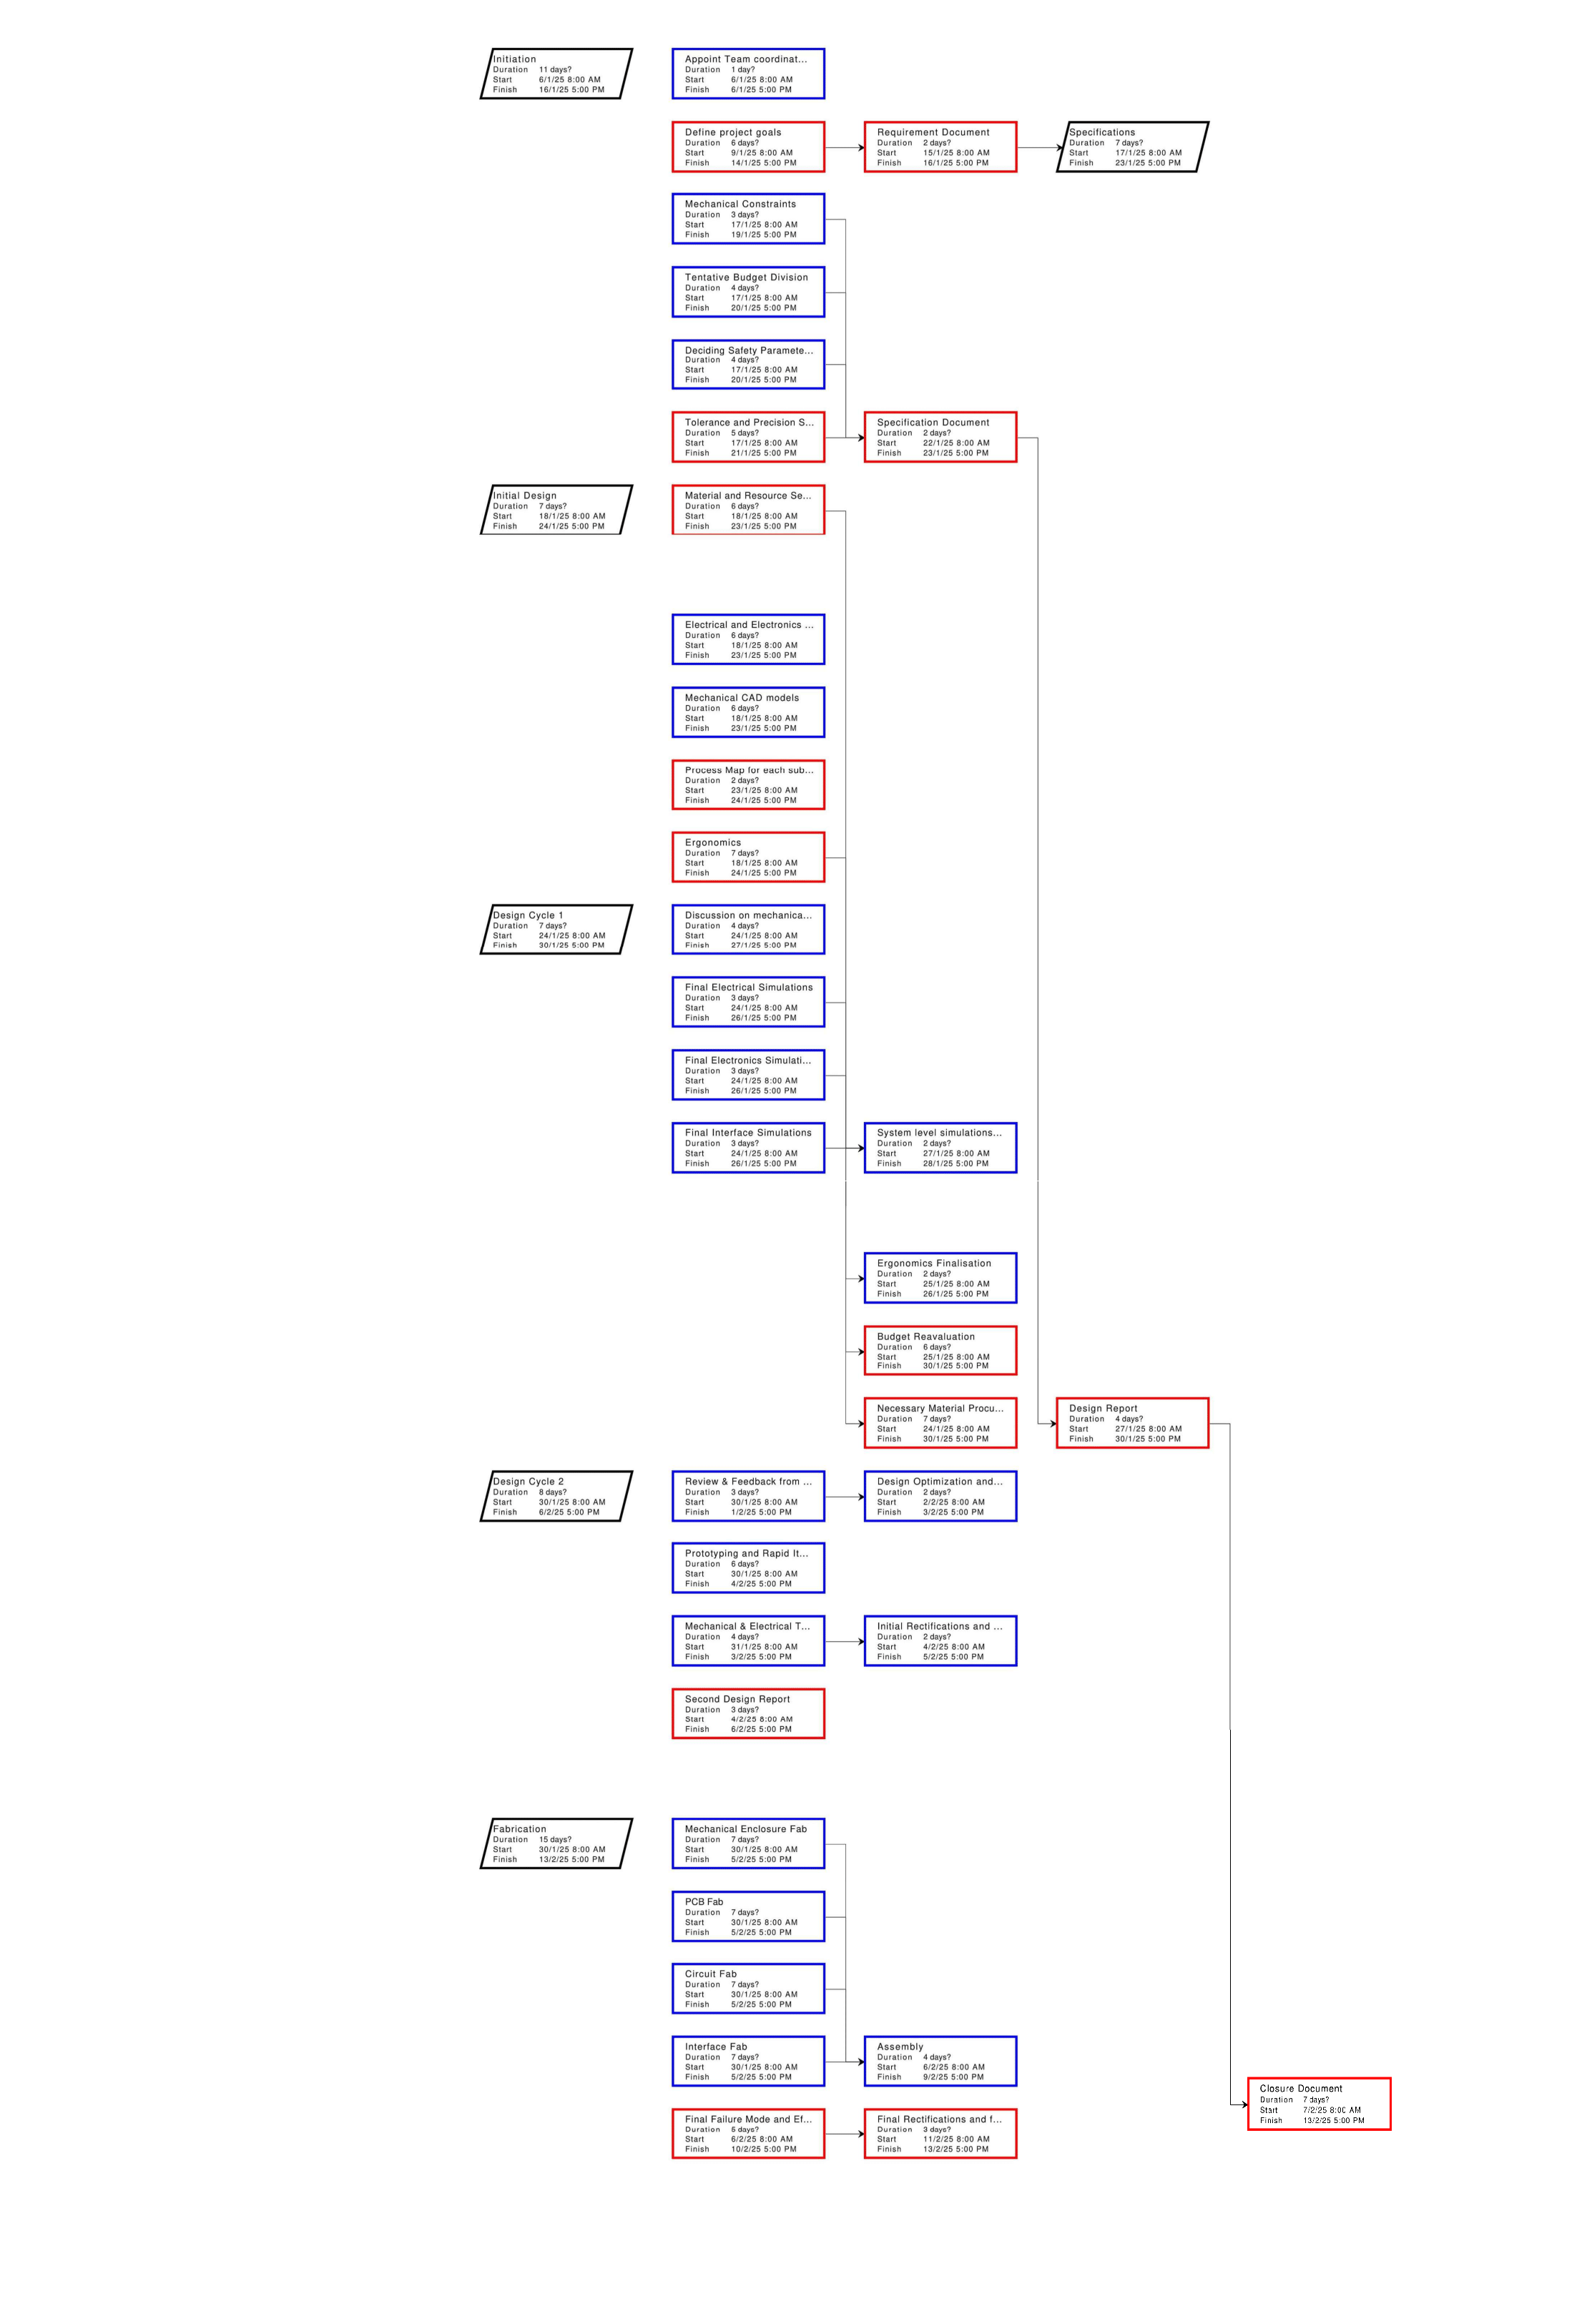
\includegraphics[width=1.2\textwidth]{network.png} % Replace with your file 
    \caption{Network Chart}
    
    \label{fig:GANTT CHART}
\end{figure}



\clearpage
\section{Design Cycle 1}
\subsection{Power Input Circuit Design}
\begin{itemize}
     

\item \textbf{Initial Goal}  To successfully simulate the circuits, determine the voltage levels of the circuit, design their generation, and configure the input
\item \textbf{Circuit Schematic} The following is the circuit schematic. We are taking in input at 5V DC from a DC power supply available in the ELP101 Lab and then converting it into -5V, 15V and -15V using the proposed circuitry
\item{Schematic}
\begin{figure}[H]
    \centering
    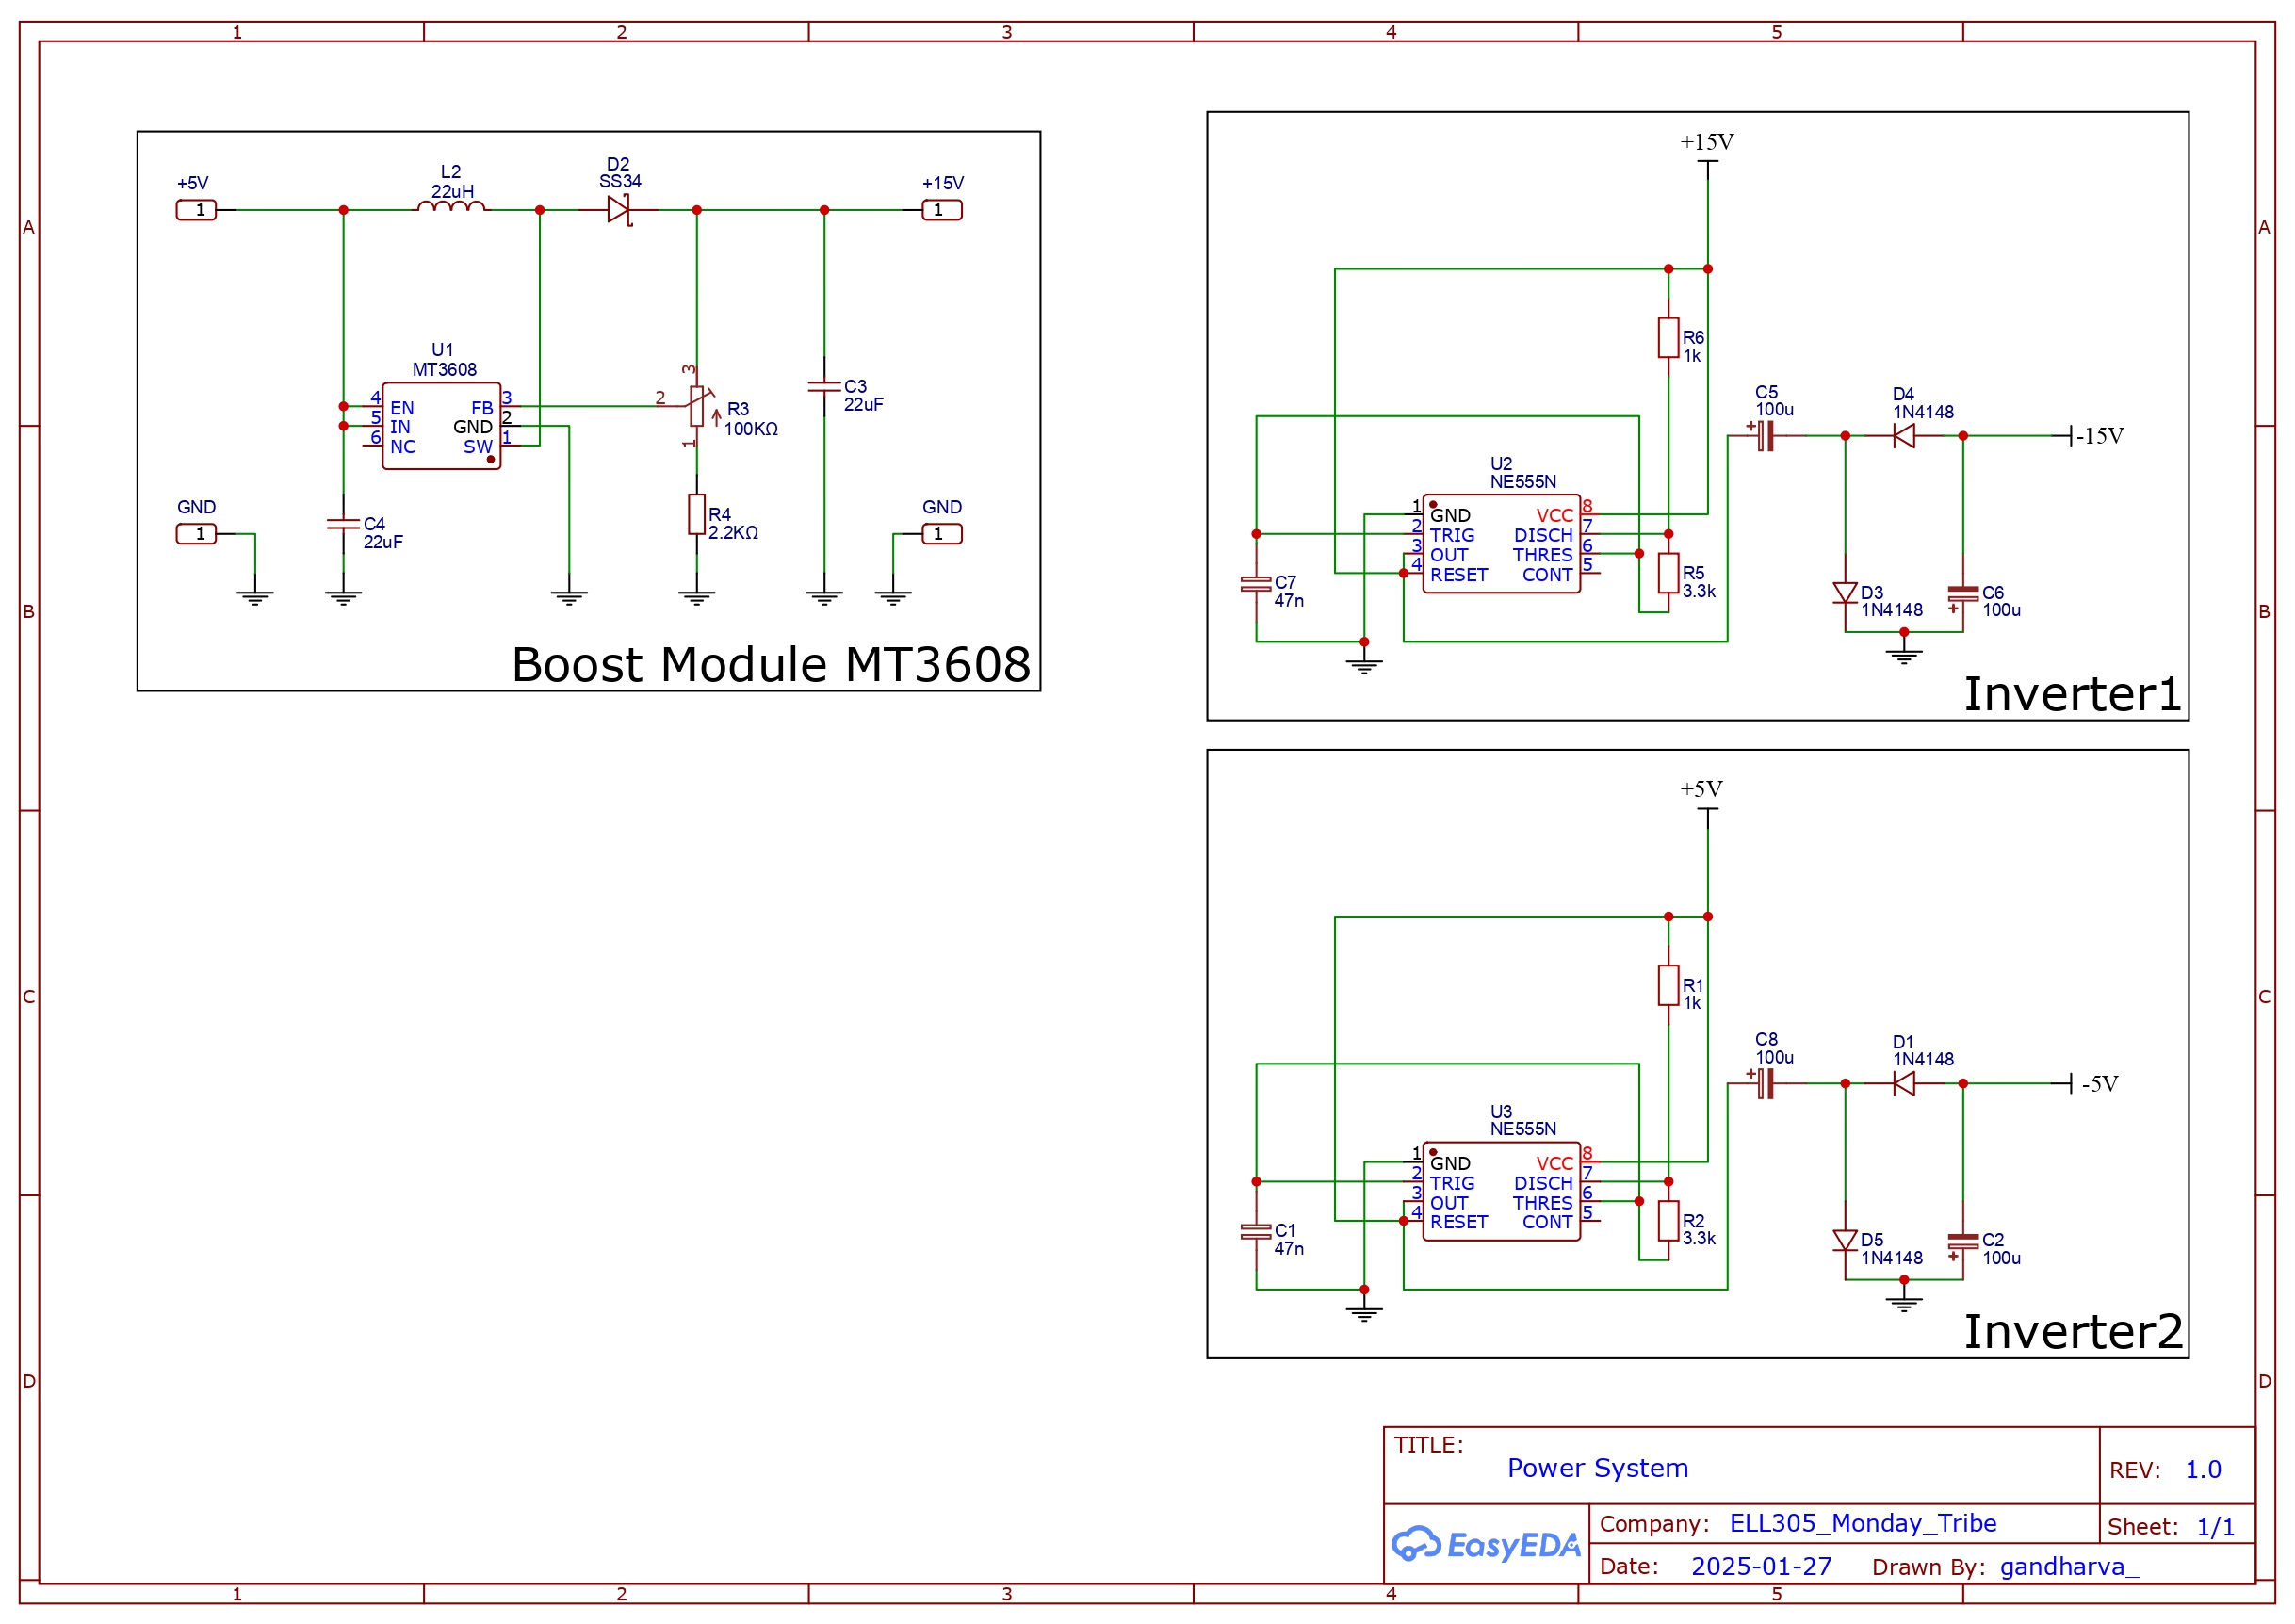
\includegraphics[width=\linewidth]{Schematic_pi_ini_2025-01-28_page-0001.jpg}
    \caption{Power Circuit Schematic}
    \label{fig:enter-label}
\end{figure}
\item \textbf{Optional Port Configuration}
The optional port \( C \) was shorted in parallel to the 4-pin main supply,determining the appropriate components for implementation

\item \textbf{Simulation of Voltage Inverter Circuit}
A voltage inverter circuit was simulated using a \( +5V \) voltage supply to achieve \( -5V \). The simulations were conducted on various software such as LTSpice, TinkerCad, and EasyEDA. However, we were only able to reach \( -4.3V \). Upon debugging, it was found that the maximum voltage of the 555 timer output itself is \( 4.3V \) due to resistive voltage drop.

Hence, a negative voltage regulator may need to be employed. This will be decided upon physically realizing the circuit next week.

Simulation link: \href{https://www.tinkercad.com/things/gf0q0Ncw5p9/editel?sharecode=jc-TJ9JB5M20FsJDGMxoH8T5PApp168cANJCAp8Wo6Q}{TinkerCad Simulation}

\item \textbf{Simulation of Boost Module}
The ability of boost module MT3608 to convert from 5V to 15V was confirmed from datasheets and its efficiency of 93percent and low output voltage ripple (less than 50mV for current drawn $<=$100mA).
Simulation link: \href{https://github.com/lisha-goel/elp305_power}{Git Repository of ELP 305 Monday Tribe Power Circuits}
\end{itemize}

\clearpage
\subsection{UI Design and Signal Generation Simulations}
\begin{itemize}
\item \textbf{Simulation Progression for Function Generator}  
 
\begin{itemize}
    \item Initially used Arduino UNO with LCD16x2 via I2C to test basic display functionality
    \item Explored different update methods to minimize flickering and optimize refresh logic
    \item Shifted to ESP32 with an OLED display for a more compact and flexible UI, allowing graphical elements like icons
\end{itemize}

\item \textbf{Signal Generation → Testing \& Validation}  
\begin{itemize}
    \item Started generating sine, square, and triangular waves using ESP32 DAC
    \item Simulated and analyzed signal stability before lab validation
    \item Integrated an op-amp stage to test amplification
\end{itemize}

\item \textbf{Control Input: Buttons → Joystick}  
\begin{itemize}
    \item Initially used push buttons for frequency and waveform selection
    \item Evaluated joystick control for smoother and more intuitive adjustments
    \item Simulated joystick-based input handling before finalizing for UI navigation
\end{itemize}

\item \textbf{BOM \& Front Panel → Hardware Integration}  
\begin{itemize}
    \item Researched and listed components, ensuring compatibility and cost-effectiveness
    \item Simulated joystick + LCD setup before confirming its usability
    \item Assessed different connector options and the feasibility of separate waveform outputs
\end{itemize}
\end{itemize}
\begin{table}[h]
    \centering
    \begin{tabular}{|l|l|}
        \hline
        \textbf{Objective} & \textbf{Simulation Link} \\
        \hline
        Display Logic for Arduino UNO (Wokwi) & \href{https://wokwi.com/projects/421519284834524161}{Link} \\
        Successful ESP32 + OLED Simulation (Wokwi) & \href{https://wokwi.com/projects/421332527375177729}{Link} \\
        Waveform Generation using ESP32 (Wokwi) & \href{https://wokwi.com/projects/421332355931919361}{Link} \\
        Use of Joystick for Intuitive UI (Wokwi) & \href{https://wokwi.com/projects/421223590526773249}{Link} \\
        \hline
    \end{tabular}
    \caption{UI and Signal Generation Simulations}
\end{table}
\clearpage
\section{Design Cycle 2}
\subsection{Revised Design}
During this week's design review and optimization phase, our electronics team has made significant improvements to the function generator's architecture compared to last week's design. The primary objective of these changes is to enhance processing speed, improve display visibility, and streamline user interaction. Below is a detailed breakdown of the modifications:

\begin{enumerate}

\item \textbf{Transition from Arduino to ESP32}
\begin{enumerate}
\item \textbf{Previous Design}: The function generator was initially designed with an Arduino microcontroller. 
\item \textbf{Updated Design}: We have replaced the Arduino with an ESP32 microcontroller.
\item \textbf{Reasoning}
\begin{enumerate}
\item \textbf{Faster Processing Speed}: ESP32 operates at a much higher clock speed (~240 MHz) compared to most Arduino boards (~16 MHz), allowing for faster waveform generation and real-time signal adjustments.
\item \textbf{Built-in DAC}: Unlike the Arduino, ESP32 has an integrated Digital-to-Analog Converter (DAC), eliminating the need for an external DAC module. This reduces hardware complexity, minimizes signal distortion, and improves output quality.
\item \textbf{Better Connectivity}: ESP32 includes built-in Wi-Fi and Bluetooth, which may be leveraged in future upgrades for wireless control and monitoring.
\end{enumerate}

\end{enumerate}



\item \textbf{Upgrade from 16x2 LCD to OLED Display}
\begin{enumerate}
\item \textbf{Previous Design}: The system used a 16x2 LCD display for waveform and settings visualization.  
\item \textbf{Updated Design}: We have replaced the LCD with an OLED display.

\item \textbf{Reasoning}
\begin{enumerate}
\item \textbf{Enhanced Visibility}: OLED displays provide a higher contrast ratio and better readability, especially in low-light conditions.

\item \textbf{Wider Viewing Angle}:Unlike LCDs, which suffer from limited viewing angles, OLEDs offer almost 180-degree visibility, making it easier for users to monitor settings from different positions.

\item \textbf{Compact and Energy Efficient}:  OLED screens are thinner and consume less power compared to LCDs, which helps optimize the overall power consumption of the function generator.

\end{enumerate}
\end{enumerate}
\item \textbf{Replacement of Push Buttons + Encoder with a Joystick
}
\begin{enumerate}
\item \textbf{Previous Design}:The user interface comprised three push buttons and a rotary encoder for navigating menus and adjusting settings.  
\item \textbf{Updated Design}:We have replaced this interface with a joystick.


\begin{enumerate}
\item \textbf{More Intuitive Operation}:A joystick allows for multi-directional control (up, down, left, right, and click), offering a more natural and user-friendly interaction compared to separate push buttons.

\item \textbf{Reduced Component Count:}:The joystick consolidates multiple functions into a single unit, reducing wiring complexity and improving the overall design compactness.


\item \textbf{Faster Adjustments}: Users can navigate menus and change waveform parameters more quickly and seamlessly, enhancing the ease of use.

\end{enumerate}
\end{enumerate}

    \item \textbf{ESP32 DAC-Based Signal Generation}  
    \begin{enumerate}
        \item Successfully generated sine and square waveforms using the ESP32 DAC.
        \item Measured output waveforms using an oscilloscope, with frequencies ranging from 10 Hz to 40 kHz.
        \item Identified minor frequency distortion and planned further optimization with timer interrupts.
    \end{enumerate}
    
    \item \textbf{Waveform Testing and Characterization}  
    \begin{enumerate}
        \item Compared ESP32-generated waveforms with AD9833 specifications.
        \item Documented waveform characteristics required for ELP101 experiments.
        \item Reference: \href{https://www.analog.com/en/products/ad9833.html}{AD9833 Product Page}
    \end{enumerate}

    \item \textbf{OLED Display Integration}
    \begin{enumerate}
        \item Successfully interfaced ESP32 with a 1.3-inch OLED display.
        \item Resolved compatibility issues by switching to the Adafruit SH110X library.
        \item Displayed test images and basic UI elements.
        \item Reference: \href{https://github.com/adafruit/Adafruit_SH110X}{Adafruit SH110X Library}
    \end{enumerate}

    \item \textbf{Bluetooth-Based Mobile App}
    \begin{enumerate}
        \item Developed a mobile app for Bluetooth-based waveform control.
        \item Established communication between the app and ESP32 for remote waveform switching.
        \item Successfully tested basic commands and waveform selection.
        \item Reference: \href{https://github.com/ThunderCodeESP32/Bluetooth}{ThunderCode ESP32 Bluetooth}
    \end{enumerate}

    \item \textbf{Consideration of Unique Selling Points (USPs)}
    \begin{enumerate}
        \item Reviewed potential USPs such as OTA updates, web server monitoring, and custom waveform generation.
        \item Evaluated feasibility based on lab requirements and hardware constraints.
        \item Shortlisted OTA updates for potential future implementation.
        \item Reference: \href{https://docs.espressif.com/projects/esp-idf/en/latest/esp32/api-reference/system/ota.html}{ESP-IDF OTA Documentation}
    \end{enumerate}

    \item \textbf{Simulation}
    \begin{enumerate}
        \item Conducted a simulation of the ESP32-based function generator.
        \item Verified OLED display and waveform output.
        \item Reference: \href{https://wokwi.com/projects/421864820253254657}{ESP32 Function Generator Simulation}
    
\end{enumerate}

\item \textbf{LTspice Simulation and RC Filter Implementation}
\begin{enumerate}
\item \textbf{Revised Design}:We created an LTspice schematic and simulated a low-pass RC filter. Additionally, we implemented this RC filter on a breadboard for testing.

\item \textbf{Reasoning}
\begin{enumerate}
\item \textbf{Signal Smoothing}:The low-pass RC filter helps in reducing high-frequency noise and achieving a cleaner signal output.


\item \textbf{Verification through simulation}:LTspice simulations allow us to analyze the frequency response and ensure proper filter behavior before physical implementation.



\item \textbf{Real-world testing}: Implementing the filter on a breadboard provides practical validation of the simulated results and helps refine circuit performance.
\item \textbf{Filter parameters}: We used a 3.19 nF capacitor and a 1 kΩ resistor to achieve a cutoff frequency of 50 kHz.
\end{enumerate}
\end{enumerate}
\item \textbf{Updated Frequency Range}
\begin{enumerate}
    \item \textbf{Revised Design}: Our function generator will provide a frequency range of 1Hz-400kHz.
    \item \textbf{Reasoning}: 
    \begin{enumerate}
        \item The manuals of ELP101 experiments were read to discover that the required frequency range of sinusoids for all the experiments is limited by 400kHz.
        \item The OpAmp LM741CN available in the lab was characterised in voltage gain configuration to provide gain stably till a frequency of 400kHz.
        \item Also, codes were run on ESP32 without the AD9833 chip, jitter-free waveforms were obtained for frequency$<=$400kHz. So consideration of possibility of using ESP-32 alone for wave generation.
    \end{enumerate}
\end{enumerate} 
\item \textbf{Inclusion of Voltage Regulator for inverting Voltage}
\begin{enumerate}
    \item \textbf{Revised Design}: For the development of the entire product and for not only demonstration purposes, circuitry involved in inverting the voltage will have to be included. For stable -15V and -5V, negative voltage regulators IC7905 AND IC7915 respectively must be integrated after the 555 timer inversion circuit.
    \item \textbf{Reasoning}:
    \begin{enumerate}
        \item On testing the circuit in lab, it was found that on giving +5V input, only -3.60V output could be obtained.
        \item  On testing the circuit in lab, it was found that on giving +15V input, only -13.80V output could be obtained.
        \item Hence a voltage regulator would be required for giving these negative voltages as supply to -Vdd for OpAmps in the offset and amplification circuitry.
        \item Lab reports of physical experiments(including pictures) are uploaded on: \href{https://github.com/lisha-goel/elp305_power}{Git Repository of ELP 305 Monday Tribe Power Circuits}
    \end{enumerate}
\end{enumerate}
\end{enumerate}
\subsection{Project Milestone Updates}
\begin{itemize}
    \item \textbf{Physical Generation of Signal : } Updated deadline - 10th February
    \item \textbf{Testing UI and Final Touches : } Updated deadline - 15th February
\end{itemize}
\subsection{Enclosure Design}
\begin{figure}[H]
    \centering
    \begin{subfigure}{0.48\textwidth} % 48% of text width
        \centering
        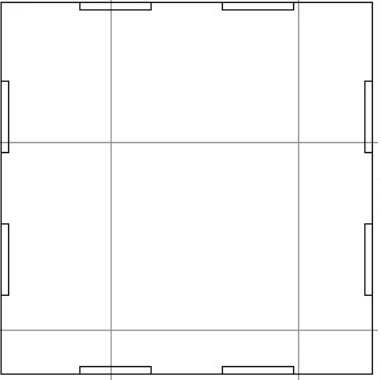
\includegraphics[width=\textwidth]{Design_Cycle_2.1.png} % Scale to fit within subfigure
        \caption{Base Panel}
        \label{fig:Base Panel}
    \end{subfigure}
    \hfill
    \begin{subfigure}{0.48\textwidth} % 48% of text width
        \centering
        \includegraphics[width=\textwidth]{Design_Cycle_2.2.jpeg} % Scale to fit within subfigure
        \caption{Front Panel}
        \label{fig:Front Panel}
    \end{subfigure}
    
    \vspace{0.5cm} % Add vertical space between rows
    
    \begin{subfigure}{0.48\textwidth} % 48% of text width
        \centering
        \includegraphics[width=\textwidth]{Design_Cycle_2.3.jpeg} % Scale to fit within subfigure
        \caption{Side Panel}
        \label{fig:Side Panel}
    \end{subfigure}
    \hfill
    \begin{subfigure}{0.48\textwidth} % 48% of text width
        \centering
        \includegraphics[width=\textwidth]{Design_Cycle_2.4.jpeg} % Scale to fit within subfigure
        \caption{Back Panel}
        \label{fig:Back Panel}
    \end{subfigure}
    
    \vspace{0.5cm} % Add vertical space between rows
    
    \begin{subfigure}{0.48\textwidth} % 48% of text width
        \centering
        \includegraphics[width=\textwidth]{Design_Cycle_2.5.jpeg} % Scale to fit within subfigure
        \caption{Top Panel}
        \label{fig:Top Panel}
    \end{subfigure}

    \caption{Enclosure Design}
    \label{fig:Enclosure Design}
\end{figure}
\newpage

\textbf{Previous Design:}  
Initially, we attempted to replicate the design of the ELP101 
 function generator without modifications.  

\textbf{Revised Design:}  
\begin{itemize}
    \item Reduced the depth of the function generator from \textbf{260mm to 190mm}.  
    \item Implemented a \textbf{sliding top mechanism} for easy access.  
\end{itemize}

\textbf{Reasoning:}  
\begin{itemize}
    \item The \textbf{sliding top} allows ELP101 students to observe the circuit more closely, improving their intuition about real-world circuit construction.  
    \item We aim to \textbf{avoid using screws} since the enclosure is made of acrylic, which could be prone to breakage.  
    \item The initial \textbf{260mm depth was excessive} given our relatively compact circuitry, so we optimized it to 190mm.  
\end{itemize}

\subsection{Updated Schematic}

\begin{figure}[H]
\centering

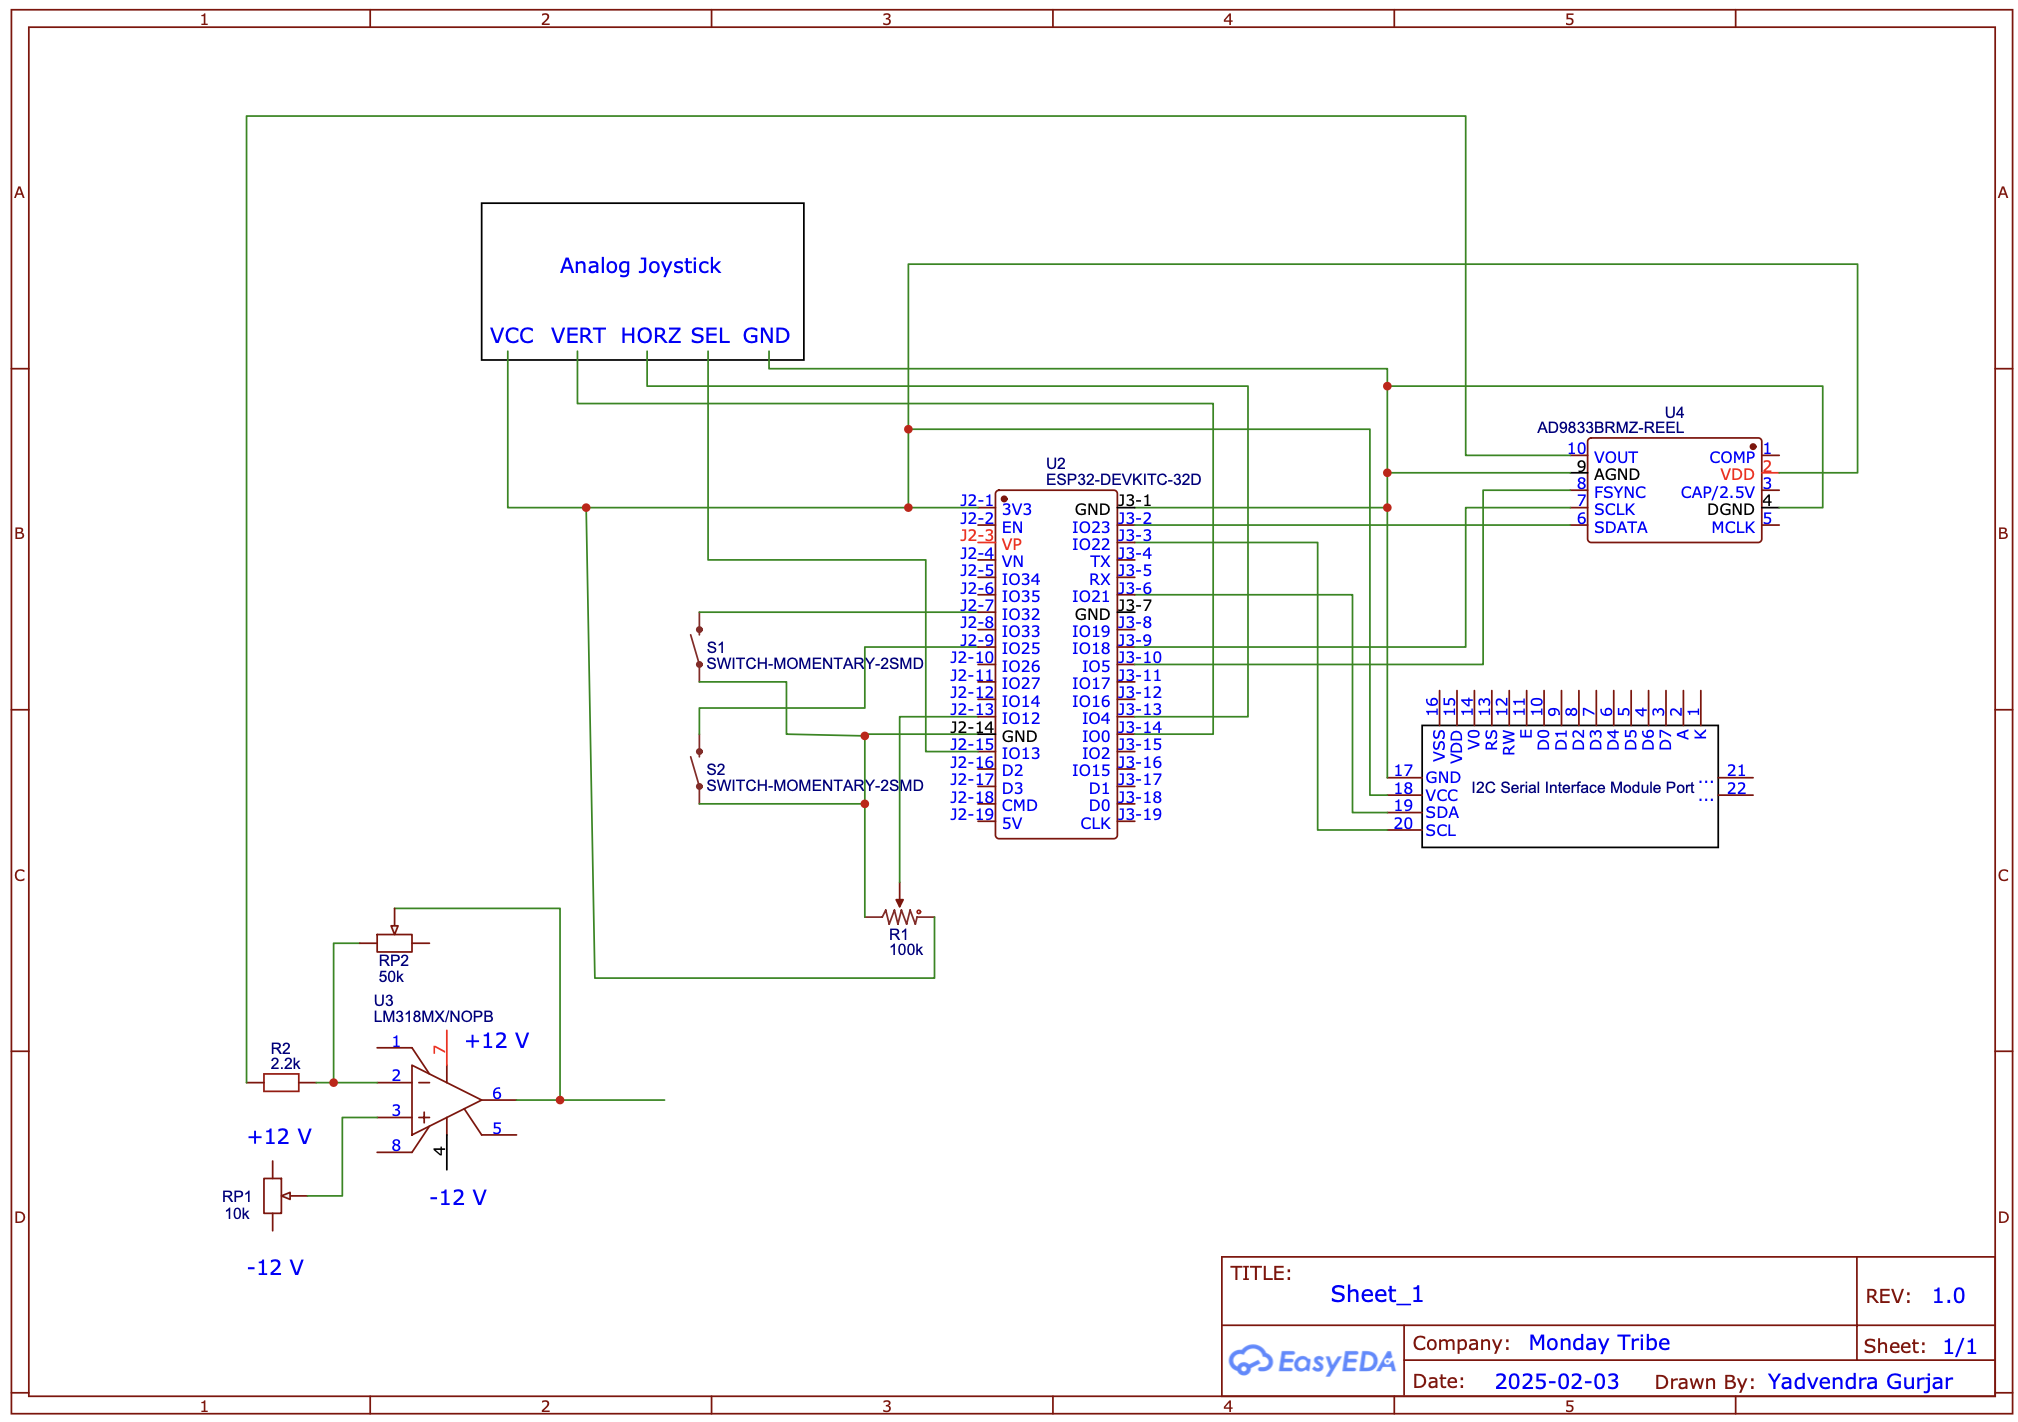
\includegraphics[width=\textwidth]{Updated Schematic.png}
\caption{Updated Schematic}
\label{fig:Updated Schematic}
\end{figure}







\clearpage
\addcontentsline{toc}{section}

% {References} % Include references in ToC
% % \bibliographystyle{apacite}
% % \bibliography{references}


\printbibliography
\clearpage


\section*{Appendix}
\addcontentsline{toc}{section}{Appendix}

\subsection*{Document ID}
\addcontentsline{toc}{subsection}{Document ID}
Major Number: 4 \\
Minor Number: 2 \\
Revision Number: 1 \\
Date (Last Modified): 06.02.25 \\
Approved By: Kriti Garg, \href{mailto:ee1221684@ee.iitd.ac.in}{ee1221684@ee.iitd.ac.in}\\
Kartikey Agarwal, \href{mailto:ee1221156@ee.iitd.ac.in}{ee1221156@ee.iitd.ac.in}
\subsection*{Document Statistics}
\addcontentsline{toc}{subsection}{Document Statistics}
\begin{tabular}{|l|l|}
\hline
\textbf{Statistic}        & \textbf{Value} \\ \hline
Word Count                & 2222          \\ \hline
Number of Sentences       & 147           \\ \hline
Number of Characters      & 15057         \\ \hline

\end{tabular}

\subsection*{Readability Indices}
\addcontentsline{toc}{subsection}{Readability Indices}
\caption{} \label{tab:List of Readability Indices}
\begin{tabular}{|l|l|}

\hline
\textbf{Index}            & \textbf{Value} \\ \hline
Readability               & Good           \\ \hline
Gunning-Fog Index         & 12           \\ \hline
Flesch-Reading Ease       & 21.99          \\ \hline
Coleman-Liau Index        & 21.97          \\ \hline

\end{tabular}
\begin{itemize}
    \item \textbf{Gunning-Fog Index}: Measures years of education needed to understand a text
    \item \textbf{Flesch-Reading Ease}: Scores readability on a 0--100 scale (higher is easier)
    \item \textbf{Coleman-Liau Index}: Estimates U.S. grade level based on letters and sentences
\end{itemize}



\clearpage
\subsection*{Minutes of Meeting}
\addcontentsline{toc}{subsection}{Minutes of Meeting}


\noindent
\textbf{Date:} 19/01/2025 \\
\textbf{Time:} 8:00 PM- 8:30 PM \\
\textbf{Venue:} Google Meet \\
\textbf{Mode:} Online \\

\vspace{0.3cm}


\subsection*{Attendees}
\begin{itemize}
    \item Dhruv Belawat
    \item Dhanashri Shivadas
    \item Lisha Goel
    \item Yagya Goyal
    \item Sushant 
    \item Gandharva Chhipa
\end{itemize}


\subsection*{Agenda}
\begin{enumerate}
  \item Required amplified outputs and viability of buck-boost converter vs. IC 7805
        \item FPGA vs. MCU: Cost, processing requirements, and built-in DAC advantages
        \item Feasibility of battery operation vs. power plug with external adapter design
\end{enumerate}

\subsection*{Resolution}
\begin{enumerate}
  \item Required amplified outputs and viability of buck-boost converter vs. IC 7805
        \item FPGA vs. MCU: Cost, processing requirements, and built-in DAC advantages
        \item Feasibility of battery operation vs. power plug with external adapter design
\end{enumerate}


\subsection*{Action Items:}
\renewcommand{\arraystretch}{1.5}
\begin{tabular}{|m{6cm}|m{4cm}|m{4cm}|}
    \hline
    \textbf{Action} & \textbf{Assigned To} & \textbf{Deadline} \\
    \hline
    Isolation Research & Yagya Goyal, Dhruv Belawat & 22/01/2025 \\
    \hline
    Power Levels Implementation & Gandharva Chippa & 22/01/2025 \\
    \hline
    Heat Management & Dhanashri Shivadas, Sushant & 22/01/2025 \\
    \hline
    Power Plug Design & Yagya Goyal & 22/01/2025 \\
    \hline
\end{tabular}



\subsection*{Next Meeting}
\begin{tabbing}
    \hspace{3cm} \= \hspace{10cm} \kill
    \textbf{Date:} \> TBD \\
    \textbf{Time:} \> TBD \\
\end{tabbing}   

\subsubsection*{Agenda for Next Meeting:}
    \begin{itemize}
        \item Review progress on assigned tasks
        \item Give the initial design to the prototyping team for testing
        \item Provide required power supply specifications to the power team
        \item Discuss challenges faced and potential solutions
        \item Plan for subsequent steps
    \end{itemize}



\textbf{Minutes Prepared By:} Samyak Jain

\subsection*{Minutes of Meeting}
%\addcontentsline{toc}{subsection}{Minutes of Meeting}


\noindent
\textbf{Date:} 20/01/2025 \\
\textbf{Time:} 3:30 - 4:00 PM \\
\textbf{Venue:} Block II 320 \\
\textbf{Meeting Facilitator:} Aditya Nagarkar \\
\vspace{0.3cm}


\subsection*{Attendees}
\begin{itemize}
    \item Kriti Garg
    \item Kartikey Agarwal
    \item Lisha Goel
    \item Aditya Sameer Nagarkar
    \item Dev Sharma
    \item Chintala Sree Varshith Reddy
    \item Madhav Gupta
    \item Gandharva Chhipa
\end{itemize}


\subsection*{Agenda}
\begin{enumerate}
    \item Distribution of tasks to various team members
    \item Since we are using DDS, the task of our team is to find out how the following things need to be implemented:
    \begin{itemize}
        \item Square Wave Analog Filtering
        \item DC Offset and Amplitude Variation
        \item Offset and Amplitude Measurement and its display on LCD panel
    \end{itemize}
\end{enumerate}




\subsection*{Action Items:}
\renewcommand{\arraystretch}{1.5}
\begin{tabular}{|m{6cm}|m{4cm}|m{4cm}|}
    \hline
    \textbf{Action} & \textbf{Assigned To} & \textbf{Deadline} \\
    
        Square Wave Analog Filtering & NA & 22/01/2025 \\
        \hline
        DC Offset and Amplitude Variation & Samyak Jain, Aarnav Singh & 22/01/2025 \\
        \hline
        Offset and Amplitude Measurement & Vikas Kumar & 22/01/2025 \\
        
     \hline
\end{tabular}




\subsection*{Next Meeting}
\begin{tabbing}
    \hspace{3cm} \= \hspace{10cm} \kill
    \textbf{Date:} \> TBD \\
    \textbf{Time:} \> TBD \\
\end{tabbing}   

\subsubsection*{Agenda for Next Meeting:}
    \begin{itemize}
        \item Review progress on assigned tasks
        \item Give the initial design to the prototyping team for testing
        \item Provide required power supply specifications to the power team
        \item Discuss challenges faced and potential solutions
        \item Plan for subsequent steps
    \end{itemize}



\textbf{Minutes Prepared By:} Samyak Jain

% \subsection*{Minutes of Meeting - Documentation }
% \addcontentsline{toc}{subsection}{Minutes of Meeting Documentation }
% \singlespacing
% \textbf{Date:} 20/01/2025 \\
% \textbf{Time:} 2:30 - 4:00 PM \\
% \textbf{Venue:} Block II 320 \\
% \textbf{Meeting Facilitator:} Dev Sharma\\
% \vspace{0.3cm}

% \subsection*{Attendees}


% \subsection*{Agenda}
% \begin{enumerate}
%     \item Review of current documentation process
%     \item Addressing issues from the previously submitted report
%     \item Assigning tasks based on the attendees' previous work on the report
%     \item Finalizing timelines for the next draft
% \end{enumerate}

% \subsection*{Action Taken:}
% \begin{enumerate}
%     \item 
%     \item Addressing issues from the previously submitted report
%     \item Assigning tasks based on the attendees' previous work on the report
%     \item Finalizing timelines for the next draft
% \end{enumerate}

\subsection*{Minutes of Meeting - Electronics Simulation }

\subsubsection*{Date}
20 January 2025

\subsubsection*{Time}
2:00 PM - 5:00 PM

\subsubsection*{Venue}
Block 2 - 320

\subsubsection*{Mode}
Offline

\subsubsection*{Attendees}
\begin{itemize}
    \item Anany Mishra
    \item Arpit Moga
    \item Arunim Garg
    \item Aryan Verma
    \item Chandan Kumar Thakur
    \item Dev Elvis Kannath
    \item Divyansh Raj Sinha
    \item Harshit Baraskar
    \item Ishu Rajput
    \item Madhav Gupta
    \item Naman Goel
    \item Prabhjit Singh
    \item Pratyush Agrawal
    \item Rakshit Sohlot
    \item Rohan Chaturvedi
    \item Saem Habeeb
    \item Sanchit Jindal
    \item Vatsal Jain
\end{itemize}

\subsubsection*{Agenda}
\begin{enumerate}
    \item Discussion on FPGA/CPLD board usage
    \item Component feasibility analysis for ELP101 function generator
    \item Finalizing display and functionality decisions
    \item Task division for simulation and interface development
\end{enumerate}

\subsubsection*{Resolution}
\begin{itemize}
    \item The AD9833 module was selected for function generation due to its simplicity and cost-effectiveness
    \item Focus shifted to Arduino Uno for simulations as ESP32’s Wi-Fi/Bluetooth features were unnecessary for the ELP101 lab
    \item Decided on a cost-effective 0.96-inch OLED display (which is around Rs.400) and avoided GLCD (which is around Rs.1,000) for budgetary reasons
    \item Sine wave plotting omitted since waveform observation can be done using a DSO
\end{itemize}

\subsubsection*{Action Taken}
Tasks were decided and distributed as follows:
\begin{itemize}
    \item \textbf{Task 1: Rotary Encoder Input and Display} 
    \begin{itemize}
        \item Dev Elvis Kannath, Ishu Rajput, Pratyush Agrawal, Rakshit Sohlot, Aryan Verma
    \end{itemize}
    \item \textbf{Task 2: Cursor Movement and Blink Effect}
    \begin{itemize}
        \item Rohan Chaturvedi, Naman Goel, Saem Habeeb, Anany Mishra
    \end{itemize}
    \item \textbf{Task 3: Measuring Peak-to-Peak Voltage}
    \begin{itemize}
        \item Arunim Garg, Harshit Baraskar, Vatsal Jain, Prabhjit Singh
    \end{itemize}
    \item \textbf{Task 4: Op-Amp Waveform Generation}
    \begin{itemize}
        \item Sanchit Jindal, Arpit Moga, Chandan Kumar Thakur, Divyansh Raj Sinha
    \end{itemize}
\end{itemize}

\subsubsection*{Date of Next Meeting}
27 January 2025

\subsection*{Minutes of Meeting - Prototyping}
\noindent
\textbf{Date:} 22 January 2025\\
\textbf{Time:} 9:30 PM - 10:00 PM \\
\textbf{Venue:} Google Meet\\
\textbf{Mode:} Online \\

\subsubsection*{Attendees}
\begin{itemize}
    \item Chintala Sree Varshith Reddy
    \item Hariom
    \item Ishaan Lakhotiya
    \item Vamika
    \item Jaya Chauhan
    \item Mitali Bhagat
\end{itemize}

\subsubsection*{Agenda}
\begin{enumerate}
    \item Discussing the existing model and its feasibility
    \item Finalizing material and structural considerations
    \item Reviewing interface and screen design
    \item Allocation of future tasks
\end{enumerate}

\subsubsection*{Resolution}
\begin{itemize}
    \item Decided to proceed with the rough idea of the current model. No major changes to avoid obstructions for the electronics team
    \item MDF metal was identified as the preferred material due to its lightweight nature, cost-effectiveness, and laser cutting compatibility. Referral to Makerspace is required for laboratory equipment compatibility
    \item ABS plastic was considered an alternative, but further research is required to determine its feasibility
    \item The LED screen size remains unchanged as it aligns with finalized requirements and budget constraints
\end{itemize}

\subsubsection*{Action Taken}
The following tasks were decided:
\begin{itemize}
    \item \textbf{Further Research on ABS Plastic:} Assigned to Jaya and Ishaan \\
    \textbf{Deadline:} 24 January 2025
    \item \textbf{Visit Makerspace:} Assigned to Vamika and Mitali. \\
    \textbf{Deadline:} 23 January 2025
    \item \textbf{Practicing Soldering:} Assigned to Shubham, Krishna, Hariom, Varshith, Vipul, Dheeraj, Aman, Teekam, Mayank, Abhineet. \\
    \textbf{Deadline:} Once every week
\end{itemize}

\subsubsection*{Action Items}
\renewcommand{\arraystretch}{1.5}
\begin{tabular}{|m{6cm}|>{\raggedright\arraybackslash}m{4cm}|m{4cm}|}
    \hline
    \textbf{Action} & \textbf{Assigned To} & \textbf{Deadline} \\
    \hline
    Doing further research on ABS plastic & Jaya, Ishaan & 24/01/2025 \\
    \hline
    Visiting Makerspace & Vamika, Mitali & 23/01/2025 \\
    \hline
    Practicing Soldering on PCBs & Shubham, Krishna, Hariom, Varshith, Vipul, Dheeraj, Aman, Teekam, Mayank, Abhineet & Once every week \\
    \hline
\end{tabular}

\subsubsection*{Date of Next Meeting}
To be decided.

\subsection*{Minutes of Meeting  of Electronics(Power)}

\noindent
\textbf{Date:} 27 January, 2025 \\
\textbf{Time:} 2:00 PM - 5:00 PM \\
\textbf{Venue:} In Lab \\
\textbf{Mode:} In-person \\

\subsubsection*{Attendees}
\begin{itemize}
    \item Lisha Goel
    \item Gandharva
    \item Sushant
    \item Dhanushree
    \item Yagya Goyal
    \item Dhruv Belawat
\end{itemize}

\subsubsection*{Agenda}
\begin{enumerate}
    \item Identify and simulate a 5V DC to ±15V and -5V circuit using boost converters and inverters
    \item Evaluate the use of the MT3608 boost converter for voltage adjustment
    \item Explore and simulate the required setup using TinkerCAD, EasyEDA, or KiCAD
    \item Understand and replicate the AE20125 Function Generator circuit for further design implementation
    \item Ensure all team members comprehend the circuit and suggest modifications
\end{enumerate}

\subsubsection*{Resolution}
\begin{enumerate}
    \item \textbf{Circuit Simulation:}
    \begin{itemize}
        \item MT3608 Boost Converter identified as a solution for converting 5V DC to the required voltage levels
        \item Two adjustment methods considered:
        \begin{itemize}
            \item Using Arduino for precise control
            \item Manual adjustment with a screwdriver
        \end{itemize}
        \item Decision: Opted for manual adjustment for simplicity and ease of implementation
    \end{itemize}
    \item \textbf{TinkerCAD Simulation:}
    \begin{itemize}
        \item Challenges noted due to limited availability of specific components, such as the MT3608 boost converter
        \item Recommendation: Use any available boost converter for preliminary simulation
        \item Alternative tools: EasyEDA or KiCAD suggested for more flexibility and accurate replication of the circuit
    \end{itemize}
    \item \textbf{Function Generator Circuit:}
    \begin{itemize}
        \item Shared a detailed description of the AE20125 Function Generator
        \item Identified the Analog Devices AD9833 as the core component for waveform generation
        \item Suggested additional tools for simulating high-frequency signal reconstruction
    \end{itemize}
    \item \textbf{Workflow Suggestions:}
    \begin{itemize}
        \item Start simulation with basic components in TinkerCAD.
        \item Transition to EasyEDA or KiCAD for more accurate circuit design and development
        \item Ensure all team members participate in understanding the circuit and provide suggestions for improvements
    \end{itemize}
\end{enumerate}

\subsubsection*{Action Taken}
\begin{enumerate}
    \item Focused on simulating and adjusting the boost converter circuit.
    \item Shared MT3608 boost converter resources and discussed configuration
    \item Transition planned to EasyEDA or KiCAD for detailed design
\end{enumerate}

\newpage
\subsubsection*{Tasks and Assignments}
\renewcommand{\arraystretch}{1.5}
\begin{table}[h!]

\begin{tabular}{|m{6cm}|>{\raggedright\arraybackslash}m{4cm}|m{4cm}|}
    \hline
    \textbf{Task} & \textbf{Assigned To} & \textbf{Deadline} \\
    \hline
    Simulate 5V DC to ±15V circuit using TinkerCAD or available tools & Dhruv Belawat, Yagya Goyal & In Lab \\
    \hline
    Replicate the circuit in EasyEDA and suggest modifications & Dhanushree & 28 Jan \\
    \hline
    Share MT3608 boost converter configuration resources & +91 77200 80121 & In Lab \\
    \hline
    Research and propose adjustments to AE20125 Function Generator & All team members & Ongoing \\
    \hline
    ELP 305(2024) I2C configuration of Real Time Clock & Yagya Goyal and Sushant & EoD \\
    \hline
\end{tabular}
\end{table}


\subsubsection*{Links Shared}
\begin{itemize}
    \item \href{https://www.instructables.com/DC-DC-Boost-Converter-MT3608/}{MT3608 Boost Converter Guide}
    \item \href{https://www.tinkercad.com/login?next=%2Fthings%2Fgf0q0Ncw5p9%2Feditel%3Fsharecode%3Djc-TJ9JB5M20FsJDGMxoH8T5PApp168cANJCAp8Wo6Q}{TinkerCAD Circuit Design}
\end{itemize}



\subsubsection*{Conclusion}
\begin{enumerate}
    \item The team will focus on simulating and adjusting the boost converter circuit
    \item Transition to EasyEDA or KiCAD for detailed design once the initial simulation is complete
    \item Collaboration will continue to ensure all components
and processes are understood
\end{enumerate}
 


\subsubsection*{Date of Next Meeting}
To be decided

\newpage
\subsection*{Minutes of Meeting for BOM and Front Design Panel}

\noindent
\textbf{Date:} 27 January, 2025 \\
\textbf{Time:} 2:00 PM - 5:00 PM \\
\textbf{Venue:} In Lab \\
\textbf{Mode:} In-person \\

\subsubsection*{Attendees}
\begin{itemize}
    \item Sanchit Jindal
    \item Arpit Moga
    \item Chandan Kumar Thakur
    \item Divyansh Raj Sinha
\end{itemize}

\subsubsection*{Agenda}
\begin{enumerate}
    \item Finalize the Bill of Materials (BOM) for the system
    \item Design a user-friendly front panel layout
    \item Explore improvements in user ergonomics for the front panel
\end{enumerate}

\subsubsection*{Resolution}
\begin{enumerate}
    \item \textbf{Bill of Materials (BOM):}
    \begin{itemize}
        \item Researched cost-effective and reliable components through online sources
    \end{itemize}
    \item \textbf{Front Panel Design:}
    \begin{itemize}
        \item Proposed replacing buttons with a joystick for easier frequency adjustments and enhanced user convenience
        \item Discussed ergonomic placement of buttons and clear labeling for improved usability
        \item Highlighted the potential to simplify the panel by reducing the number of buttons without compromising functionality
        \item Finalized button size as 6x6x8 mm and labeled functions (e.g., Power, Menu, Reset)
        \item Drafted a front panel design balancing aesthetics and functionality
    \end{itemize}
    \item \textbf{Joystick Implementation:}
    \begin{itemize}
        \item Simulated a joystick with an LCD16x2 setup, confirming smoother usability compared to buttons
        \item Found the joystick's built-in button capable of replacing the waveform selector button and encoder, simplifying the design
    \end{itemize}
\end{enumerate}

\subsubsection*{Action Taken}
\begin{itemize}
    \item Decided to configure and test the joystick setup on an ESP32 in the next session
\end{itemize}

\subsubsection*{Date of Next Meeting}
To be decided

\subsection*{Minutes of Meeting for ESP32 and OLED Simulation}

\noindent
\textbf{Date:} 27 January, 2025 \\
\textbf{Time:} 2:00 PM - 5:00 PM \\
\textbf{Venue:} In Lab \\
\textbf{Mode:} In-person \\

\subsubsection*{Attendees}
\begin{itemize}
    \item Rohan Chaturvedi
    \item Naman Goel
    \item Saem Habeeb
    \item Anany Mishra
\end{itemize}

\subsubsection*{Agenda}
\begin{enumerate}
    \item  Recreate Arduino + LCD16x2 functionality on an ESP32 with a 0.96-inch OLED display
    \item Enhance UI aesthetics and functionality on the OLED interface
    \item Reserve DAC pins on the ESP32 for potential signal generation tasks
\end{enumerate}

\subsubsection*{Resolution}
\begin{enumerate}
    \item \textbf{OLED Interface Design:}
    \begin{itemize}
         \item Explored libraries for rendering icons or logos to create a more visually appealing OLED interface
        \item Selected a smaller 0.96-inch OLED display for cost-efficiency, as minimal information needs to be displayed
        \item Decided to replicate existing LCD16x2 functionality before incorporating additional features
    \end{itemize}
    \item \textbf{ESP32 Pin Configuration: }
    \begin{itemize}
        \item Reserved DAC pins (25/26) for potential use in signal generation tasks
    \end{itemize}
    \item \textbf{Code and Compatibility:}
    \begin{itemize}
        \item Initially attempted Micropython but switched to C for better compatibility with other team codes
        \item Reconfigured connections and adapted code to integrate the ESP32 with the OLED display
    \end{itemize}
\end{enumerate}
\subsubsection*{Action Taken}
\begin{itemize}
      \item Successfully replicated all LCD16x2 features on the OLED interface
    \item Enhanced the UI with improved spacing and reserved the possibility for adding icons in future iterations
\end{itemize}
\subsubsection*{Date of Next Meeting}
To be decided


\subsection*{Minutes of Meeting for Signal Generation and Testing}
\noindent
\textbf{Date:} 27 January, 2025 \\
\textbf{Time:} 2:00 PM - 5:00 PM \\
\textbf{Venue:} In Lab \\
\textbf{Mode:} In-person \\

\subsubsection*{Attendees}
\begin{itemize}
    \item Arunim Garg
    \item Harshit Baraskar
    \item Prabhjit Singh
    \item Vatsal Jain

\end{itemize}


\subsubsection*{Agenda}
\begin{enumerate}
    \item Simulate and test sine, square, and triangular signal generation using ESP32, a power supply, and opamp
    \item Evaluate the performance of ESP32-generated signals and compare them to the AD9833 module for Function Generator (FG)
    \item Test various waveforms and document their characteristics including amplitude and frequency ranges
    \item Resolve configuration issues with Arduino IDE for ESP32 and consider switching to PlatformIO for future testing
    \item Finalize the FG design and validate using opamp-based amplification circuits
\end{enumerate}

\subsubsection*{Resolution}
\begin{enumerate}
    \item The team decided to test ESP32-generated signals (sine, triangular, and sawtooth) on the Wokwi simulation platform to understand their performance
    \item It was agreed to evaluate the performance of ESP32 DAC and compare it with AD9833 to assess its cost-saving advantage
    \item The team faced configuration challenges with Arduino IDE, leading to the decision to use PlatformIO for future trials
    \item The decision was made to simulate opamp-based amplification circuits and document the results for future lab sessions
\end{enumerate}

\subsubsection*{Action Taken}
\begin{enumerate}
    \item Developed and tested code for generating sine, triangular, and sawtooth waveforms on Wokwi simulation
    \item Successfully simulated and documented the results of the signal generation task on Wokwi
    \item Despite challenges, initial testing was conducted with Arduino IDE, and future trials are planned with PlatformIO
    \item Simulated the opamp-based amplification circuits and prepared documentation for future lab validations
    \item Next steps: Proceed with lab testing to finalize the FG design and verify its feasibility for ELP101 experiments
\end{enumerate}



\subsubsection*{Date of Next Meeting}
To be decided


\subsection*{Minutes of Meeting for Optimization of Simulation Code (Wokwi)}
\noindent
\textbf{Date:} 27 January, 2025 \\
\textbf{Time:} 2:00 PM - 5:00 PM \\
\textbf{Venue:} In Lab \\
\textbf{Mode:} In-person \\

\subsubsection*{Attendees}
\begin{itemize}
    \item Aryan Verma
    \item Dev Elvis Kannath
    \item Ishu Rajput
    \item Pratyush Agrawal
    \item Rakshit Sohlot
    
\end{itemize}

\subsubsection*{Agenda}
\begin{enumerate}
    \item Minimize screen flickering and optimize display update logic for the simulation code
    \item Reduce excessive use of \texttt{lcd.clear} and refine frequency conversion logic
    \item Improve the overall user experience by minimizing cursor blinking and retaining leading zeros in the frequency display
    \item Fix the bug where unwanted characters appear when encoder values drop below zero
\end{enumerate}

\subsubsection*{Resolution}
\begin{enumerate}
    \item The team proposed maintaining a record of displayed characters and updating only the necessary changes, reducing the need for frequent \texttt{lcd.clear} calls
    \item Discussed the impact of continuously blinking cursors on user experience and agreed to minimize cursor activity to specific interactions only
    \item Decided to retain leading zeros in the frequency display to improve clarity and avoid unnecessary format changes that may hinder usability
    \item Identified a bug caused by frequency alteration logic where unwanted characters appeared when encoder values dropped below zero. A fix was decided upon to address this issue
\end{enumerate}

\subsubsection*{Action Taken}
\begin{enumerate}
    \item Successfully disabled continuous cursor blinking by adding \texttt{lcd.noBlink()} in strategic places and optimized the display logic by removing unnecessary \texttt{lcd.clear} statements
    \item Improved the screen's performance, reducing flickers and enhancing the overall user experience
    \item Implemented a function to convert \texttt{freqStr} to a float, fixing bugs and ensuring that the display format remains consistent for better readability
    \item Finalized the simulation code for the Arduino UNO board, with plans to integrate it with other task outputs if the board remains the final choice for the product
\end{enumerate}


\subsubsection*{Date of Next Meeting}
To be decided

\subsection*{Minutes of Meeting for Electronics(Power)}

\subsubsection*{Date}
26 January 2025

\subsubsection*{Time}
6:00 PM - 6:30 PM

\subsubsection*{Venue}
Online (Google Meet)

\subsubsection*{Mode}
Online

\subsubsection*{Attendees}
\begin{itemize}
    \item Lisha Goel
    \item Sushant
    \item Gandharva Chippa
\end{itemize}

\subsubsection*{Agenda}
\begin{enumerate}
    \item Evaluate methods to achieve ±15V supply from the available 5V DC supply
    \item Discuss the feasibility of using USB Type C versus a 4-pin configuration
    \item Analyze and identify suitable IC modules for design enhancement
\end{enumerate}

\subsubsection*{Resolution}
\begin{itemize}
    \item \textbf{Boost Converter and Amplifier:}
    \begin{itemize}
        \item Gandharva suggested using a boost converter for achieving higher voltage levels
        \item Agreed on using high-quality boost converters to ensure a stable output
    \end{itemize}
    \item \textbf{USB Type C Discussion:}
    \begin{itemize}
        \item Considered the use of a PD trigger module (20V) for USB Type C implementation
        \item Evaluated the power ratings and standardization challenges of USB Type C for continuous operation devices
    \end{itemize}
    \item \textbf{Voltage Regulation:}
    \begin{itemize}
        \item Discussed the necessity of a voltage regulator to maintain a stable 5V supply
    \end{itemize}
    \item \textbf{MT3608 IC Module:}
    \begin{itemize}
        \item Agreed on using the MT3608 IC module for voltage boost applications
        \item Shared relevant resources for understanding the specifications and performance of the MT3608 IC
    \end{itemize}
    \item \textbf{General Conclusions:}
    \begin{itemize}
        \item +5V DC supply is the starting point
        \item Boost converters and two inverters (derived from the same op-amp IC) are required for the design
    \end{itemize}
\end{itemize}

\subsubsection*{Action Taken}
\begin{itemize}
    \item Shared resources for the MT3608 IC module and discussed its applications
    \item Finalized the need to explore potential issues related to frequency performance of op-amps and boost converters
\end{itemize}

\subsubsection*{Date of Next Meeting}
To be decided

\subsection*{Minutes of Meeting for prototyping}

\subsubsection*{Date}
28 January 2025

\subsubsection*{Time}
9:00 PM - 9:30 PM

\subsubsection*{Venue}
Google Meet

\subsubsection*{Mode}
Online

\subsubsection*{Attendees}
\begin{itemize}
    \item Chintala Sree Varshith Reddy
    \item Hariom
    \item Aman
    \item Vamika
    \item Jaya Chauhan
    \item Teekam
    \item Shubham
    \item Vipul
    \item Mayank
    \item Dheeraj
    \item Krishna Sendhvil
    \item Abhineet
\end{itemize}

\subsubsection*{Agenda}
\begin{enumerate}
    \item Progress update on RD Works and design finalization
    \item Development tasks for the front and back panel
    \item Work distribution for soldering and design teams
    \item Lab visit planning and task allocation
\end{enumerate}

\subsubsection*{Resolution}
\begin{itemize}
    \item The front panel design has been finalized
    \item Lab visits have been scheduled for both the design and soldering teams
    \item Task distribution between the design and soldering teams has been discussed
    \item Frequency dials will be replaced with joysticks without major design modifications
    \item A demo front panel will be created in the lab tomorrow
    \item Soldering team members are encouraged to practice as no active soldering tasks are pending
\end{itemize}

\subsubsection*{Action Taken}
\begin{itemize}
    \item The finalized front panel design will be shared in the group
    \item Material selection: Acrylic sheet (4 mm thickness, made by joining two 2 mm sheets)
    \item The structure will be tested to ensure it supports component weight
    \item The design team will focus on RD Works and creating the front panel in the lab
    \item The soldering team will practice circuit soldering and demonstrate it to the TA
    \item Timings for the next lab visit have been confirmed for both teams
\end{itemize}

\subsubsection*{Date of Next Meeting}
To be scheduled after lab visit and initial testing

\subsection*{Minutes of Meeting for Core Team Meet}

\subsubsection*{Date}
29 January 2025

\subsubsection*{Time}
8:00 PM - 9:00 PM

\subsubsection*{Venue}
Google Meet

\subsubsection*{Mode}
Online

\subsubsection*{Chairperson}
Kriti

\subsubsection*{Attendees}
\begin{itemize}
    \item Dev
    \item Aditya
    \item Lisha
    \item Gandharva
    \item Varshith
\end{itemize}

\subsubsection*{Agenda}
\begin{enumerate}
    \item Set milestones for design
    \item Finalisation of Involvement factor
    \item Appraisal discussion
    \item The requirements of Documentation Team
\end{enumerate}

\subsubsection*{Resolution}
\begin{itemize}
    \item Dev suggested for deciding the milestones that the milestones should be easy on the feasibility side and that the team should try to simplify
    \item The following Milestones of design were suggested by Aditya :
    \begin{itemize}
        \item Generation of signal
        \item Amplification - DC offset
        \item Enclosure design and heat management front panel User Interface
        \item Testing and final touches
    \end{itemize}
    \item Varshith came up with the milestone of frequency resolution.
    \item Prototyping update (by Varshith):
    \begin{itemize}
        \item Front panel demo was attempted today
        \item Issue 1 : Component dimensions needed → Will be acquired on Monday
        \item Issue 2 : Acrylic might break with screws
        \item Enclosure design will follow Madhav's specifications
        \item Individual front panel components will be completed by Wednesday, but full assembly may require additional time
    \end{itemize}
    \item Circuitry update (by Aditya)
    \begin{itemize}
         \item Attempt will be made using a personal ESP32 module
         \item Issue: Lab’s ESP32 was not functioning
         \item For signal generation code is ready and should be completed within an hour
         \item Amplification part is not ready yet and requires further work
    \end{itemize}
    \item Power input update (by Lisha)
    \begin{itemize}
        \item Circuit has been built
        \item Simulation is almost functional but improvement is needed with physical components
        \item Issues : Not inverting fully and no regulator is available and also team is currently unaware of debugging
    \end{itemize}
    \item Aditya suggested that if the code using ESP's DAC worked properly then they should use that else they would have to use AD9833
    \item The following requirements of Documentation were submitted by Dev
    \begin{itemize}
        \item Specifications and requirements update
        \item Milestones update and the milestones of this design cycle
        \item Latest minutes of meet to be submitted
        \item Final Involvement factor list
        \item Project Management updates to be submitted
        \item References should be put forward and cross checked
    \end{itemize}
    \item Portability Concern:
    \begin{itemize}
        \item Gandharva: Why not make the design portable?
        \item Varshith: The probability of breaking is high, especially at the joints
        \item Gandharva: It won’t break if we round the corners
        \item Lisha: Type-C connection makes it portable and allows data transfer from a laptop
        \item Lisha: If we make it portable, everything changes, and the rack-size design may not be relevant anymore
    \end{itemize}
    \item The following were the USP suggestions :
    \begin{itemize}
        \item Lisha suggested Wifi connectivity for linked functionality
        \item Dev suggested Voltmeter to measure voltage at certain nodes
    \end{itemize}
    \item Enclosure and Assembly discussion :
    \begin{itemize}
        \item Gandharva suggested that the team should make largest area face openable and the team agreed
        \item Until the assembly is finalised deciding on dimensions is not possible
        \item Gandharva suggested of having two ports but remarked that there must be enough space for that
        \item Power Connections Discussion: Considering C-pin and 4-pin speaker connector for power
    \end{itemize}
\end{itemize}

\subsection*{Minutes of Meeting for Design}
\noindent
\textbf{Date:} 2 February, 2025 \\
\textbf{Time:} 10:00 - 11:00 PM \\
\textbf{Venue:} Google Meet \\
\textbf{Mode:} Online \\

\subsubsection*{Attendees}
\begin{itemize}
    \item Kriti Garg
    \item Kartikey Agrawal
    \item Lisha Goel
    \item Madhav
    \item Dev Sharma
    \item Gandharva Chhipa
    \item Aditya Nagarkar
    \item Varshith
\end{itemize}

\subsubsection*{Referenced Documents}
\begin{itemize}
    \item \href{https://docs.google.com/spreadsheets/u/0/d/1mf3VolONgFL6qE_bgLDeh4sSy1PNTC3in6jEBaED-h8/edit}{Evaluation\_Monday\_tribe}
    \item \href{https://docs.google.com/spreadsheets/u/0/d/1uf0n1ec6wdD89DGu6o5pDTRil8vPTHQxd6ou25UlpaI/edit}{Team\_Workspace}
    \item \href{https://docs.google.com/document/u/0/d/1IVD8nQkdYI0tBmnchBCmUj0YVEVN_2yDqmUBOeMQ9xg/edit}{Tribe\_Feedback}
\end{itemize}

\subsubsection*{Agenda}
Deciding a plan of action for the upcoming week.
\begin{longtable}{|l|l|}
    \hline
    \textbf{Topic} & \textbf{Team Member} \\
    \hline
    Enclosure  & Varshith \\
    \hline
    Final Simulations   & Madhav \\
    \hline
    Schematics   & Lisha Goel, Aditya Nagarkar \\
    \hline
\end{longtable}

\subsubsection*{Key Decision}
The team will maintain parallel review of the last submitted report alongside current work, documenting all changes at each stage of development.
\subsection*{Minutes of Meeting for Power}

\textbf{Date:}February 2, 2025\\
\textbf{Time}7:30 PM - 8:10 PM\\
\textbf{Venue}Online\\
\textbf{Mode}Online\\

\subsubsection*{Attendees}
\begin{itemize}
    \item Lisha Goel
    \item Sushant
    \item Gandharva Chippa
    \item Dhruv Belawat
    \item Dhanashri Shivadas
    \item Yagya Goyal
    \item Divyanshu
    \item Aarnav Singh
\end{itemize}

\subsubsection*{Agenda}
\begin{enumerate}
    \item Task allocation for lab work.
    \item Op-Amp testing and data collection.
    \item Documentation and submission deadlines.
    \item Progress review and methodology discussion.
\end{enumerate}

\subsubsection*{Resolution}
\begin{itemize}
    \item Lab work tasks were distributed among members.
    \item Testing procedure for the operational amplifier was finalized.
    \item Key parameters for Op-Amp testing were determined, including frequency range (100Hz to 1MHz), input and output voltage, and waveform documentation.
    \item Implementation plans were set based on Op-Amp results.
    \item Documentation requirements and submission deadlines were established.
\end{itemize}

\subsubsection*{Action Taken}
\begin{itemize}
    \item Task allocations for lab work:
          \begin{itemize}
              \item Inverter circuit implementation: Dhanashri & Dhruv.
              \item Boost module input/output, offset, amplitude, and frequency controlling circuit verification & testing: Yagya, Divyanshu & Aarnav.
              \item 5V supply integration & powering via capacitor: Sushant & Gandharva.
              \item End-of-lab group review & innovation discussion: Open to all members.
          \end{itemize}
    \item Sushant & Gandharva to check Op-Amp functionality and record:
          \begin{itemize}
              \item Frequency range: 100Hz to 1MHz.
              \item Input and output voltage (Vp/p).
              \item Capture and document waveform shapes.
              \item Follow the basic amplifier circuit setup.
          \end{itemize}
    \item Post-lab actions:
          \begin{itemize}
              \item Sushant to upload Op-Amp output images.
              \item Dhruv Belawat to add software details.
              \item Dhanashri to complete the section on the necessity of a voltage regulator.
              \item All members ensure proper documentation in the shared file.
          \end{itemize}
\end{itemize}

\subsubsection*{Date of Next Meeting}
To be scheduled after completion of lab work and review of the documentation.


\subsection*{Minutes of Meeting}
\textbf{Date:} February 2, 2025\\
\textbf{Time:} 7:30 PM - 8:10 PM\\
\textbf{Mode:} Online\\

\subsubsection*{Attendees}
\begin{itemize}
    \item Lisha Goel
    \item Sushant
    \item Gandharva Chippa
    \item Dhruv Belawat
    \item Dhanashri Shivadas
    \item Yagya Goyal
    \item Divyanshu
    \item Aarnav Singh
\end{itemize}

\subsubsection*{Agenda}
\begin{enumerate}
    \item Task Allocation for Lab Work.
    \item Op-Amp Testing and Data Collection.
    \item Documentation and Submission Deadlines.
    \item Progress Review and Methodology Discussion.
\end{enumerate}

\subsubsection*{Discussion Points and Action Items}
\begin{enumerate}
    \item \textbf{Task Allocation for Lab Work}
    \begin{itemize}
        \item Inverter Circuit Implementation: Dhanashri \& Dhruv.
        \item Boost Module Input/Output, Offset, Amplitude \& Frequency Controlling Circuit Verification \& Testing: Yagya, Divyanshu \& Aarnav.
        \item 5V Supply Integration \& Powering via Capacitor: Sushant \& Gandharva.
        \item End-of-Lab Group Review \& Innovation Discussion: Open to all members.
    \end{itemize}
    
    \item \textbf{Op-Amp Testing and Data Collection}
    \begin{itemize}
        \item Sushant \& Gandharva were assigned to check the working of the operational amplifier.
        \item The following parameters were to be recorded:
        \begin{itemize}
            \item Frequency range: 100Hz to 1MHz.
            \item Input and Output Voltage (Vp/p).
            \item Capture and document waveform shapes.
            \item Follow basic amplifier circuit setup.
        \end{itemize}
    \end{itemize}
    
    \item \textbf{Implementation}
    \begin{itemize}
        \item Based on the testing of the Op-Amp, which is required in all the circuits, others will implement their corresponding circuits and note the waveforms and results.
    \end{itemize}
    
    \item \textbf{End Actions Required}
    \begin{itemize}
        \item Sushant to upload Op-Amp output images.
        \item Dhruv Belawat to add software details.
        \item Dhanashri to complete the section on the necessity of a voltage regulator.
        \item All members to ensure proper documentation in the shared file.
    \end{itemize}
\end{enumerate}

\subsubsection*{Conclusion}
The meeting successfully allocated tasks for the lab session, outlined testing procedures, and established documentation requirements with clear deadlines.
\subsubsection*{Date of Next Meeting}
To be scheduled after completion of lab work and review of the above tasks.


\subsection*{Minutes of Meeting for prototyping}

\textbf{Date:}February 4, 2025\\
\textbf{Time} 2:00 PM - 3:30 PM\\
\textbf{Venue}Block II-320 \\
\textbf{Mode}In person\\

\subsubsection*{Attendees}
\begin{itemize}
    \item Chintala Sree Varshith Reddy
    \item Jaya Chauhan
    \item Krishna Sendhvil
    \item Ishaan
    \item Vamika
    \item Teekam
    \item Dheeraj
\end{itemize}

\subsubsection*{Agenda}
\begin{enumerate}
    \item Assembly of parts of the demo model.
    \item Verifying the operation of measured dimensions of front panel components.
\end{enumerate}

\subsubsection*{Resolution}
\begin{itemize}
    \item Successfully assembled the demo model for the sliding design, ensuring full functionality and stability.
    \item Created a demo front panel with updated dimensions, verifying that all components fit properly.
\end{itemize}

\subsubsection*{Action Taken}
\begin{itemize}
    \item The prototype was assembled using chloroform and the sliding mechanism was tested.
    \item Created a demo front panel with updated dimensions and verified component placement accuracy.
\end{itemize}

\subsubsection*{Date of Next Meeting}
To be scheduled based on further tests and refinements.
\subsection*{Minutes of Meeting for protyping}

\textbf{Date:}February 4, 2025\\
\textbf{Time} 4 PM - 5 PM\\
\textbf{Venue}Block II-320 \\
\textbf{Mode}In person\\

\subsubsection*{Attendees}
\begin{itemize}
    \item Chintala Sree Varshith Reddy
    \item Hariom
    \item Aman
    \item Vamika
    \item Jaya Chauhan
    \item Teekam
    \item Shubham
    \item Vipul
    \item Mayank
    \item Dheeraj
    \item Krishna Sendhvil
    \item Abhineet
    \item Ishaan
    \item Mitali
\end{itemize}

\subsubsection*{Agenda}
\begin{enumerate}
    \item Conduct measurements on the equipment and develop the overall box design.
    \item Discuss and decide on the locking mechanism for the slider.
    \item Create a demo model for the proposed design to check functionality.
\end{enumerate}

\subsubsection*{Resolution}
\begin{itemize}
    \item Finalized dimensions for all holes in the front panel for components such as the joystick, OLED, and push buttons.
    \item Completed the RD Works file and successfully laser-cut the model.
    \item Finalized the locking mechanism for the slider.
\end{itemize}

\subsubsection*{Action Taken}
\begin{itemize}
    \item Measured equipment purchased by the TA, including the OLED, joystick, and push buttons.
    \item Brainstormed and decided on a stopper mechanism with an acrylic piece for the slider lock.
    \item Created an RD Works file for the demo model featuring a sliding top design.
    \item Conducted laser cutting of parts in the lab.
    \item Assigned a backup team to design an alternative model in RD Works in case the sliding mechanism was unsatisfactory.
\end{itemize}

\subsubsection*{Date of Next Meeting}
February 6, 2025 (Thursday) 


\subsection*{Action Items by Team}
\subsubsection*{Prototyping Team (Lead: Varshith)}
\begin{enumerate}
    \item Develop sliding box mechanism
    \begin{itemize}
        \item Implement side and top panel trials
        \item Complete component measurements for front panel precision
    \end{itemize}
\end{enumerate}

\subsubsection*{Simulation Team (Lead: Madhav)}
\begin{enumerate}
    \item ESP Development
    \begin{itemize}
        \item Implement multicore simulation
        \item Execute code on ESP hardware
        \item Investigate Bluetooth integration (lower priority)
    \end{itemize}
    \item Achieve basic signal generation functionality
    \item Develop peripheral circuit
\end{enumerate}

\subsubsection*{Circuitry Team (Lead: Aditya)}
\begin{enumerate}
    \item ESP Alternative Planning
    \begin{itemize}
        \item Evaluate AD9833 as backup solution
        \item Complete all schematics by 3:30 PM
    \end{itemize}
    \item Circuit Development
    \begin{itemize}
        \item Design and implement Op-Amp circuit
        \item Integrate DC Offset functionality
        \item Team: Aditya, Lisha, Gandharva, Madhav
    \end{itemize}
\end{enumerate}

\subsubsection*{Power Team (Lead: Lisha)}
\begin{enumerate}
    \item Power Supply Development
    \begin{itemize}
        \item Implement and test inverter circuit
        \item Evaluate efficiency metrics
        \item Procure negative voltage regulator (IC7905) if needed
    \end{itemize}
    \item Order speaker connectivity components
\end{enumerate}

\subsubsection*{Documentation Team (Lead: Dev)}
\begin{enumerate}
    \item Update bill of materials
    \item Document meeting minutes (current and next day)
    \item Complete references section
    \item Integrate recent changes into existing report
\end{enumerate}

\subsubsection*{Pending Items for Faculty Confirmation}
\begin{enumerate}
    \item Design Cycle 2 expectations
    \item Prototype documentation requirements
    \item Demonstration schedule
\end{enumerate}

\subsubsection*{Team-wide Decisions Needed}
\begin{enumerate}
    \item Enclosure size optimization (Big Box vs Small Box)
    \item Design Cycle 2 milestone finalization
\end{enumerate}

\subsubsection*{Design Cycle II Milestones}
\begin{enumerate}
    \item Basic circuit assembly
    \item Output impedance measurement
    \item Bluetooth functionality integration
\end{enumerate}

\subsubsection*{Technical Notes}
\begin{itemize}
    \item \textbf{ESP Implementation Strategy:}
    \begin{itemize}
        \item Primary focus on multi-core functionality
        \item Signal generation isolation on dedicated core
    \end{itemize}
    \item \textbf{Circuit Priorities:}
    \begin{itemize}
        \item Op-Amp circuit optimization critical
        \item DC Offset integration within Op-Amp circuit
        \item Peripheral circuit assignment to simulation team
    \end{itemize}
\end{itemize}

\subsection*{Minutes of Meeting}
\begin{itemize}
    \item \textbf{Date}: 3 February 2025
    \item \textbf{Time}: 3:30-4:45 PM
    \item \textbf{Venue}: Block II 320
    \item \textbf{Meeting Facilitator}: Aditya Nagarkar
\end{itemize}

\subsubsection*{Attendees}
\begin{itemize}
    \item Aditya Nagarkar
    \item Jay Kumar
    \item Rishit Jaiswal
    \item Sahaj Jain
    \item Aditya Vijay
    \item Vikas Kumar
    \item Yadvendra Gurjar
\end{itemize}

\subsubsection*{Agenda}
\begin{enumerate}
    \item Distribution of Tasks to various team members:
    \begin{itemize}
        \item Schematics have to be made of ESP generation certificates using EasyEDA. (Vikas, Tejas, Yadvendra)
        \item Documentation to be made and sent to documentation team (Jay, Sahaj, Rishit)
        \item Make a RC LPF of 50 kHz or 1 kHz (Rishit, Sahaj, Jay)
        \item Mind Map (Samyak)
        \item MOM (Rishit)
    \end{itemize}
\end{enumerate}

\subsubsection*{Action Items}
\begin{longtable}{| p{8cm} | p{6cm} |}
\hline
\textbf{Task} & \textbf{Assigned To} \\
\hline
\endfirsthead
\hline
\textbf{Task} & \textbf{Assigned To} \\
\hline
\endhead
\hline
Schematics need to be created for ESP generation certificates using EasyEDA. & Tejas, Vikas, Yadvendra \\
\hline
Design an RC low-pass filter to smooth the step sine wave. & Rishit, Sahaj Jain, Jay Kumar \\
\hline
Documentation needs to be prepared and sent to the documentation team. & Jay Kumar, Sahaj Jain, Rishit \\
\hline
Create a mind map outlining the project flow. & Samyak \\
\hline
\end{longtable}

\subsubsection*{Next Meeting}
\begin{itemize}
    \item \textbf{Date}: TBD
    \item \textbf{Time}: TBD
\end{itemize}

\subsubsection*{Minutes Prepared By}
Rishit Jaiswal

\subsection*{Minutes of Meeting}
\begin{itemize}
    \item \textbf{Date}: 3 February 2025
    \item \textbf{Time}: 2:00-5:00 PM
    \item \textbf{Venue}: Block II 320
    \item \textbf{Meeting Facilitator}: Madhav Gupta
\end{itemize}

\subsubsection*{Attendees}
\begin{itemize}
    \item Sanchit Jindal
    \item Arpit Moga
    \item Divyansh Raj Sinha
    \item Chandan Kumar Thakur
    \item Arunim Garg
    \item Harshit Baraskar
    \item Prabhjit Singh
    \item Vatsal Jain
    \item Saem Habeeb
    \item Anay Mishra
    \item Rohan
    \item Rakshit
    \item Naman 
    \item Ishu Rajput
    \item Pratyush Agrawal
    \item Aryan Verma
    \item Dev Elvis
\end{itemize}

\subsubsection*{Agenda}
\begin{enumerate}
    \item Design Thinking
    \begin{itemize}
        \item Evaluated the feasibility of Bluetooth control for waveform switching.
        \item Assessed security concerns regarding unauthorized Bluetooth access and implemented a manual override.
        \item Decided against adding icons to OLED due to limited screen size.
        \item Identified the impact of waveform generation delays and the need for timer interrupts.
        \item Assessed the necessity of the AD9833 module.
        \item Reviewed feasibility of additional functionalities: Web Server, OTA updates, Custom Waveform Generation.
    \end{itemize}
    \item Implementation
    \begin{itemize}
        \item Established Bluetooth communication between ESP32 and mobile app.
        \item Integrated ESP32 with OLED and optimized UI readability in simulation. 
        \item Programmed waveform generation and analyzed frequency distortion using an oscilloscope.
        \item Updated OLED library to Adafruit SH110X for 1.3-inch display compatibility.
        \item Documented waveform characteristics required for ELP101.
        \item Compared ESP32-generated waveforms with AD9833 specifications.
        \item Reviewed potential USPs and filtered non-essential features.
    \end{itemize}
\end{enumerate}

\subsubsection*{Discussions and Decisions Taken}
\begin{enumerate}
    \item Web Server & Monitoring (By Sanchit)
    \begin{itemize}
        \item Pros: Remote monitoring, error detection, power saving, and improved instructor control.
        \item Cons: Not all students have mobile devices, potential misuse by other groups.
        \item Decision: Not prioritized due to limited usability in the lab setting.
    \end{itemize}
    \item Over-the-Air (OTA) Updates (By Divyansh)
    \begin{itemize}
        \item Necessary for scalability and usability.
        \item Pros: Faster updates, remote management, and future-proofing.
        \item Cons: Security risks, Wi-Fi reliability, and hardware dependencies.
        \item Decision: Should be included to streamline firmware updates in multiple devices.
    \end{itemize}
    \item Custom Signal Generation (By Arpit)
    \begin{itemize}
        \item Pros: Greater flexibility and future-proofing.
        \item Cons: Higher complexity, increased complexity, and not required for ELP-101 experiments.
        \item Decision: Not necessary for this project due to lack of lab requirements.
    \end{itemize}
    \item Signal Generation & Analysis (By Arunim, Harshit, Prabhjit, Vatsal)
    \begin{itemize}
        \item Tested waveform generation on actual hardware, to assess the necessity of AD9833
        \item Performed Fourier analysis and identified frequency distortions.
        \item Reviewed ELP101 lab requirements and cross-checked specifications.
    \end{itemize}


\begin{table}[h!]
\centering
\begin{tabular}{|c|c|c|c|}
\hline
\textbf{Sno} & \textbf{Type of Wave} & \textbf{Amplitude} & \textbf{Frequency} \\
\hline
1 & Sine Wave & 8.6V & 1000Hz \\
2 & Sine Wave & 8.6V & 1126Hz \\
3 & Sine Wave & 8.6V & 1526Hz \\
4 & Sine Wave & 10V & 500Hz \\
5 & Sine Wave & 1.8V & 500Hz \\
6 & Sine Wave & 2.92V & 1000Hz \\
7 & Sine Wave & 2V & 40KHz \\
8 & Sine Wave & 1.16V & 1000Hz \\
9 & Sine Wave & 2.04V & 40KHz \\
10 & Sine Wave & 2.24V & 1000Hz \\
11 & Sine Wave & 2.20V & 1000Hz \\
12 & Sine Wave & 10.1V & 10Hz \\
13 & Sine Wave & 9.9V & 1000Hz \\
\hline
\end{tabular}
\caption{Signals used during our ELP101 course taken from our submitted reports}
\end{table}

    \item OLED Display Implementation (By Group 3)
    \begin{itemize}
        \item Encountered library incompatibility issues; resolved using Adafruit SH110X.
        \item Successfully displayed test images; further work required for full UI integration.
    \end{itemize}
    \item ESP32 Bluetooth Communication with Mobile App (By Group 1)
    \begin{itemize}
        \item Developed mobile app for Bluetooth waveform switching.
        \item Tested integration between ESP32 and the app.
    \end{itemize}
    \item Integration of ESP32+OLED with Waveform Generation (By Group 2)
    \begin{itemize}
        \item Integrated ESP32 I/O with waveform generation.
        \item Implemented button inputs using interrupts.
        \item Utilized ESP32's dual-core feature for multitasking.
    \end{itemize}

\end{enumerate}

\subsubsection*{Pending Tasks}
\begin{enumerate}
    \item Design Thinking
    \begin{itemize}
        \item Finalize AD9833 module decision after further hardware testing.
        \item Optimize waveform generation using timer interrupts.
        \item Assess OTA update impact on shared lab usability.
        \item Define Web Server monitoring scope and feasibility.
    \end{itemize}
    \item Implementation
    \begin{itemize}
        \item Implement timer-based waveform control.
        \item Test complete waveform generation code with OLED UI.
        \item Integrate and compare AD9833 module with ESP32’s DAC.
        \item Prototype OTA updates and Web Server monitoring.
        \item Conduct final performance testing and documentation.
    \end{itemize}
\end{enumerate}

\end{document}
